\chapter{Effect of minimal attractive correlation in the bath}
\label{siam-attr-chap}

\section{The modified hamiltonian}
We will include a local particle-hole symmetric correlation of strength \(U_b\) on the origin of the lattice:
\begin{equation}\begin{aligned}
	\mathcal{H} = \sum_{k\sigma}\epsilon_k \tau_{k\sigma} + \epsilon_d \left( \hat n_{d \uparrow} - \hat n_{d \downarrow} \right) ^2 + \sum_{k\sigma} \left(V_{k} c^\dagger_{k\sigma} c_{d\sigma} + h.c.\right) +J \vec{S_d}\cdot\vec{s} - U_b\left(\hat n_{0 \uparrow} - \hat n_{0 \downarrow}\right)^2 
\end{aligned}\end{equation}

\begin{figure}[!htb]
	\centering
	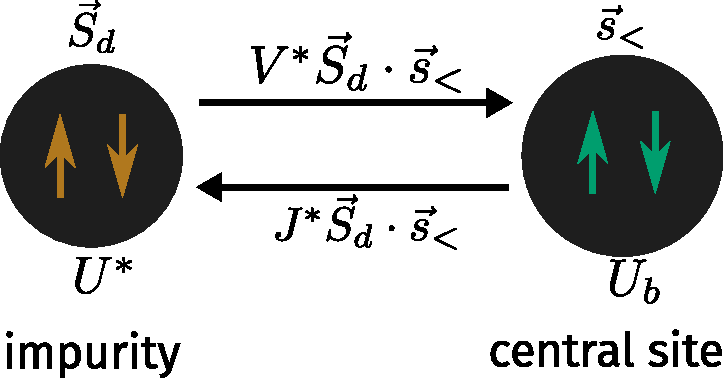
\includegraphics[width=0.5\textwidth]{../figures/zeromode.pdf}
	\caption{While we have studied the full model under renormalisation group, often we will turn to a simplified zero-bandwidth version of the model that is obtained by ignoring the kinetic energy part of the Hamiltonian. This zero-bandwidth model is effectively a two site model.}
\end{figure}

\section{RG Equations}

The derivation of the RG equations are shown in appendix~\ref{app-derivation}.
. \(n_j\) is the number of \(k-\)states at the \(j^\text{th}\) isoenergetic shell. 
\begin{gather}
	\Delta U_b = 0, ~ ~\Delta U = 4V^2 n_j\left(\frac{1}{d_1} - \frac{1}{d_0}\right) - n_j\left(\frac{J^2}{d_2} - \frac{K^2}{d_3}\right),\label{rg-eq1}\\
	\Delta V = -\frac{3n_j V}{8}\left[\left(J + 4U_b/3\right) \left(\frac{1}{d_2} + \frac{1}{d_1}\right) + \left(K + 4U_b/3\right)\left(\frac{1}{d_3} + \frac{1}{d_0}\right)\right],\label{rg-eq2}\\
	\Delta J = -\frac{n_j J\left(J + 4U_b\right)}{d_2},~ ~\Delta K = -\frac{n_j K\left(K + 4U_b\right)}{d_3}\label{rg-eq3}
\end{gather}

The denominators are
\begin{equation}\begin{aligned}
	d_0 = \omega - \frac{D}{2} + \frac{U_b}{2} - \frac{U}{2} + \frac{K}{4}, \quad d_1 = \omega - \frac{D}{2} + \frac{U_b}{2} + \frac{U}{2} + \frac{J}{4}, \quad d_2 = \omega - \frac{D}{2} + \frac{U_b}{2} + \frac{J}{4}, \quad d_3 = \omega - \frac{D}{2} + \frac{U_b}{2} + \frac{K}{4}
\end{aligned}\end{equation}

\paragraph{Important points regarding notation}
\begin{itemize}
	\item The labels \(U_0,J_0,V_0\) that may occur in the axes of the plots or anywhere else represent the bare values of the couplings \(U,J\) and \(V\). 
	\item Throughout the upcoming results, the bare value of \(U_b\) is set to the negative of the bare value of \(U_0\): \(U_b = -U_0/10\). This means that whenever we vary \(U_0\) along the axis of a plot, we are simultaneous varying \(U_b\).	
\end{itemize}

\section{Phase diagram}

\begin{center}
	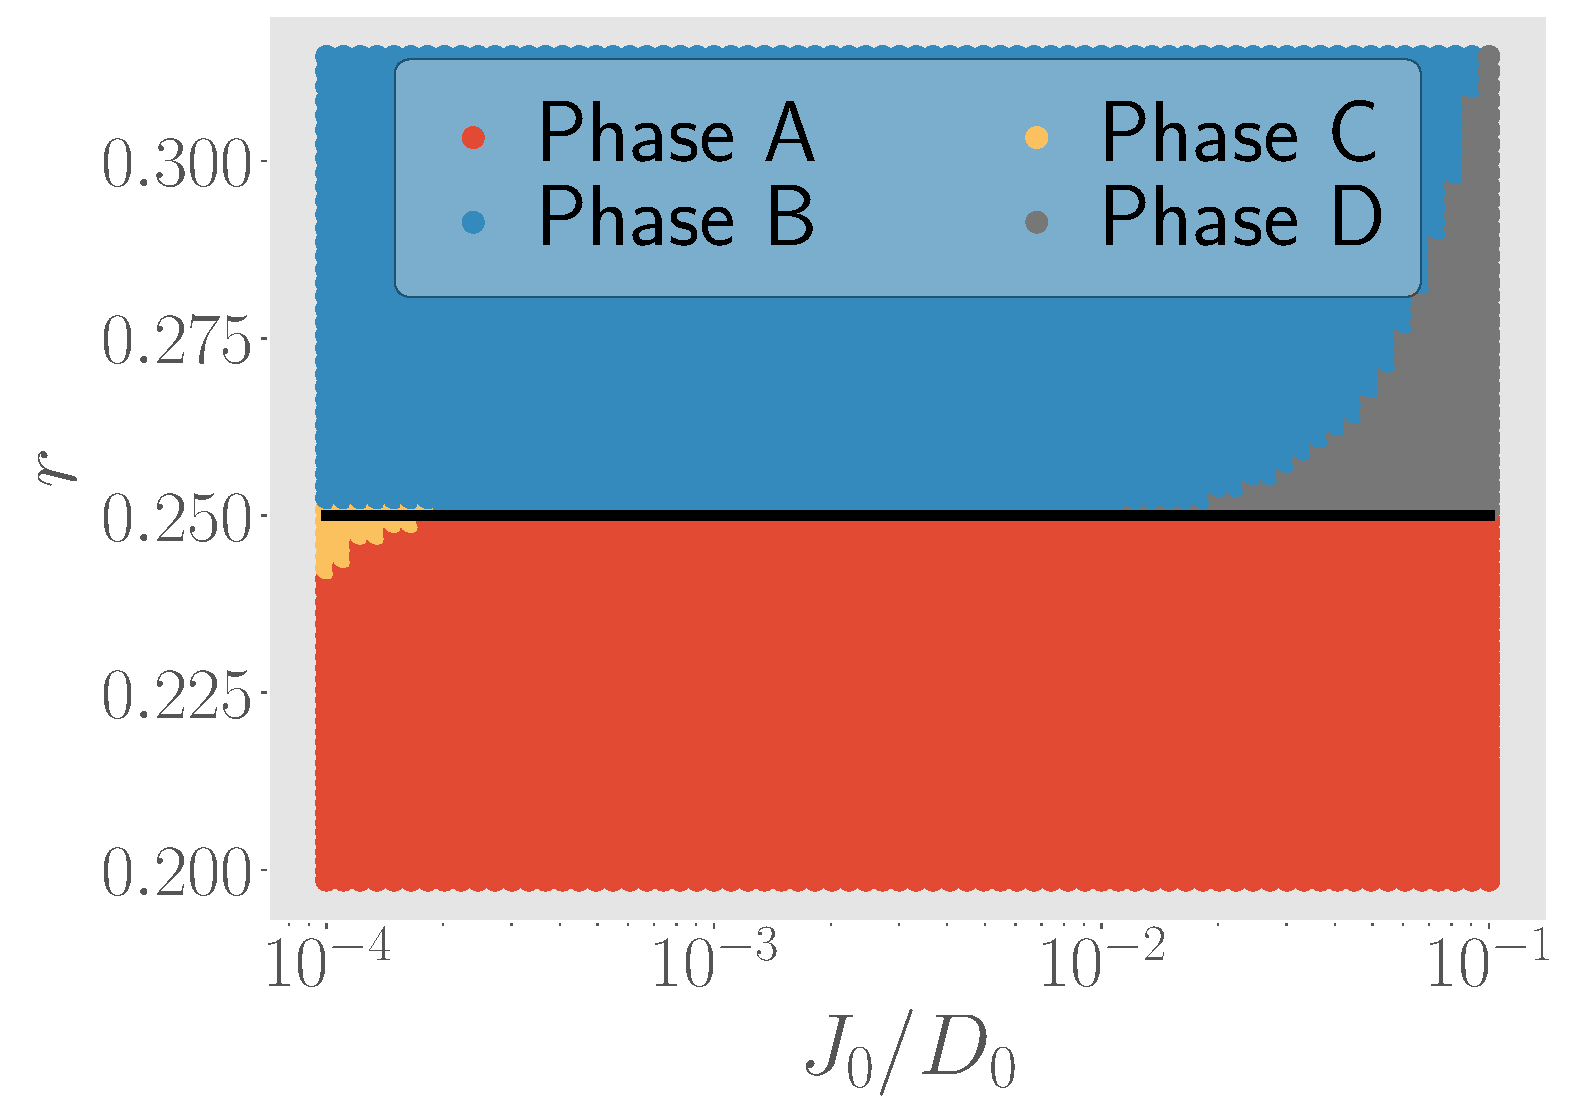
\includegraphics[width=0.9\textwidth]{../figures/phase-map-MIT.pdf}
\end{center}

\begin{center}
\begin{tabular}{|c|c|c|c|c|}
\hline
phase & RG flow & fixed point & GS & 2-site GS \\ 
\hline
blue & \(\Delta U <0, \Delta J,\Delta V>0\) & \(U^* \ll V^* \ll J^*\) & SS & \(\ket{SS}=\ket{\uparrow,\downarrow} - \ket{\downarrow, \uparrow}\)  \\ 
green &  \(\Delta U < 0, \Delta J < 0,\Delta V>0\) & \(J^* < U^* \ll V^*\) & SS + CT-0 & \(c\ket{SS} + \sqrt{1-c^2}\ket{CT-0}\)  \\  
red &  \(\Delta U > 0, \Delta J,\Delta V<0\) & \(U^* \gg 1,  V^* = J^* = 0\) & decoupled LM & \(\left\{\ket{\uparrow}, \ket{\downarrow} \right\} \otimes \left\{\ket{0}, \ket{2}\right\} \) \\
gray &  \(\Delta U, \Delta J,\Delta V < 0\) & \(U^* = V^* = J^* = 0\) & lattice & \(\left\{\ket{\uparrow}, \ket{\downarrow}, \ket{0}, \ket{2} \right\} \otimes \left\{\ket{0}, \ket{2}\right\}\) \\
\hline
\end{tabular}
\end{center}

\section{Evolution of the groundstate across the transition}

\subsection*{Overlap of ground state against spin singlet and charge triplet zero states}
\begin{center}
	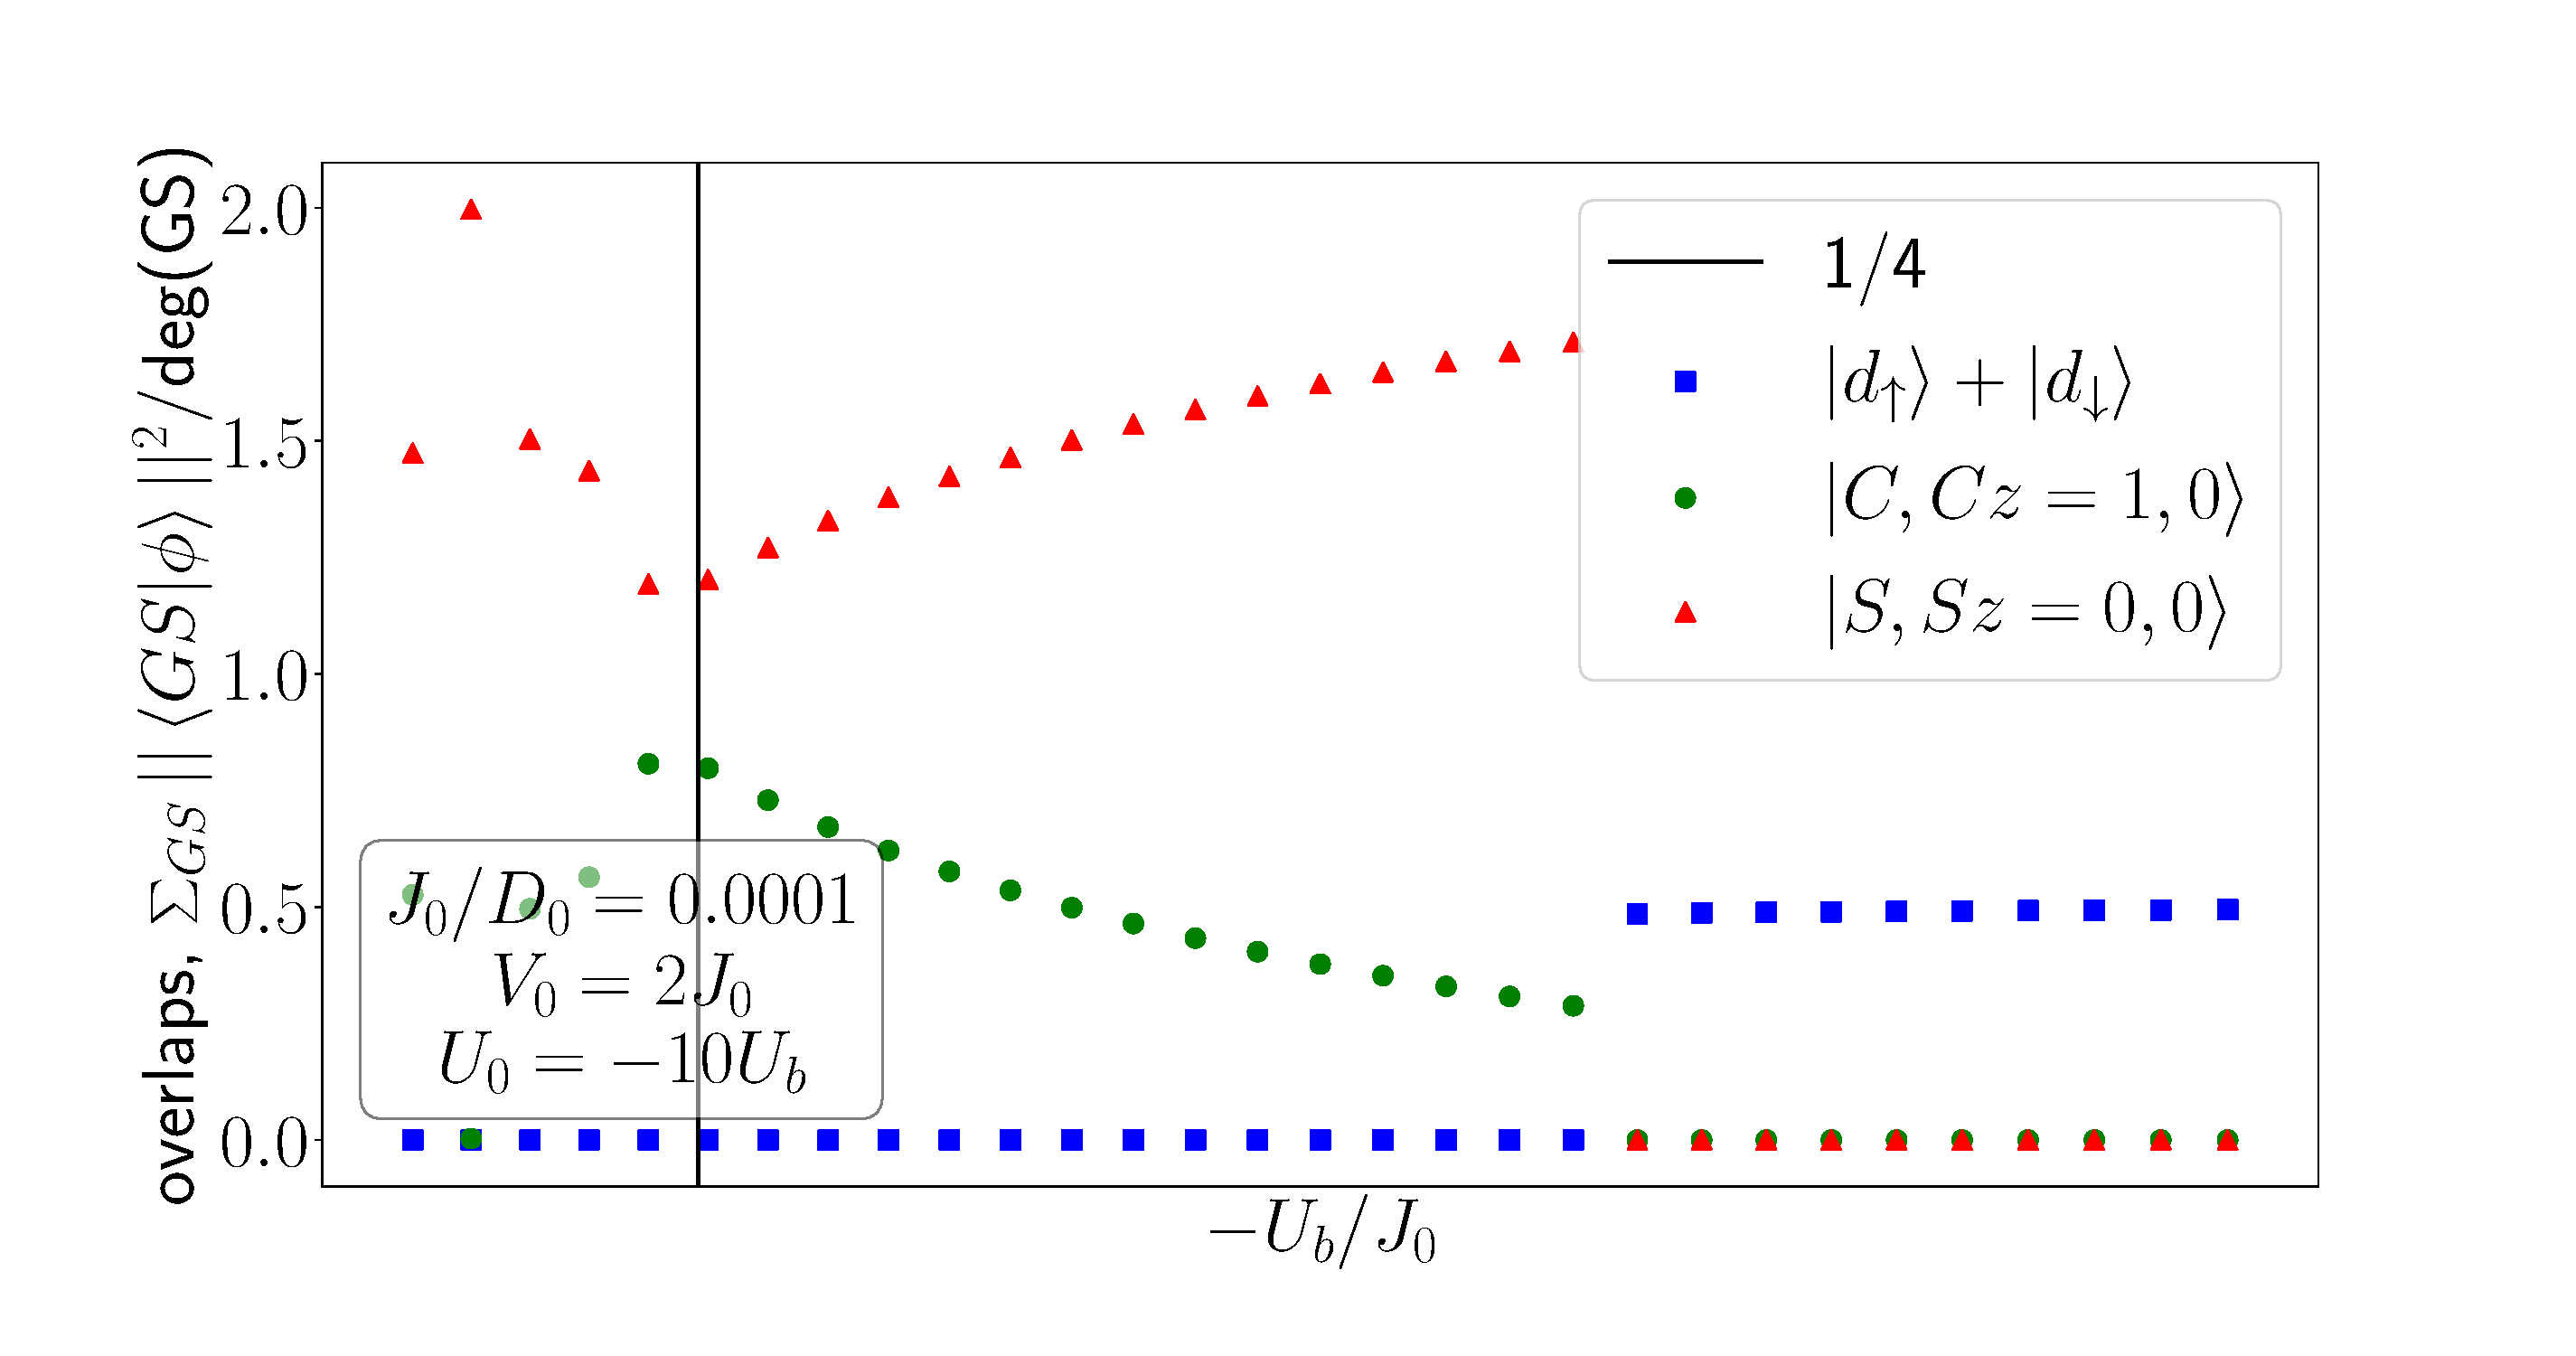
\includegraphics[width=0.7\textwidth]{../figures/overlaps_gs-J=0.100.pdf}\\
	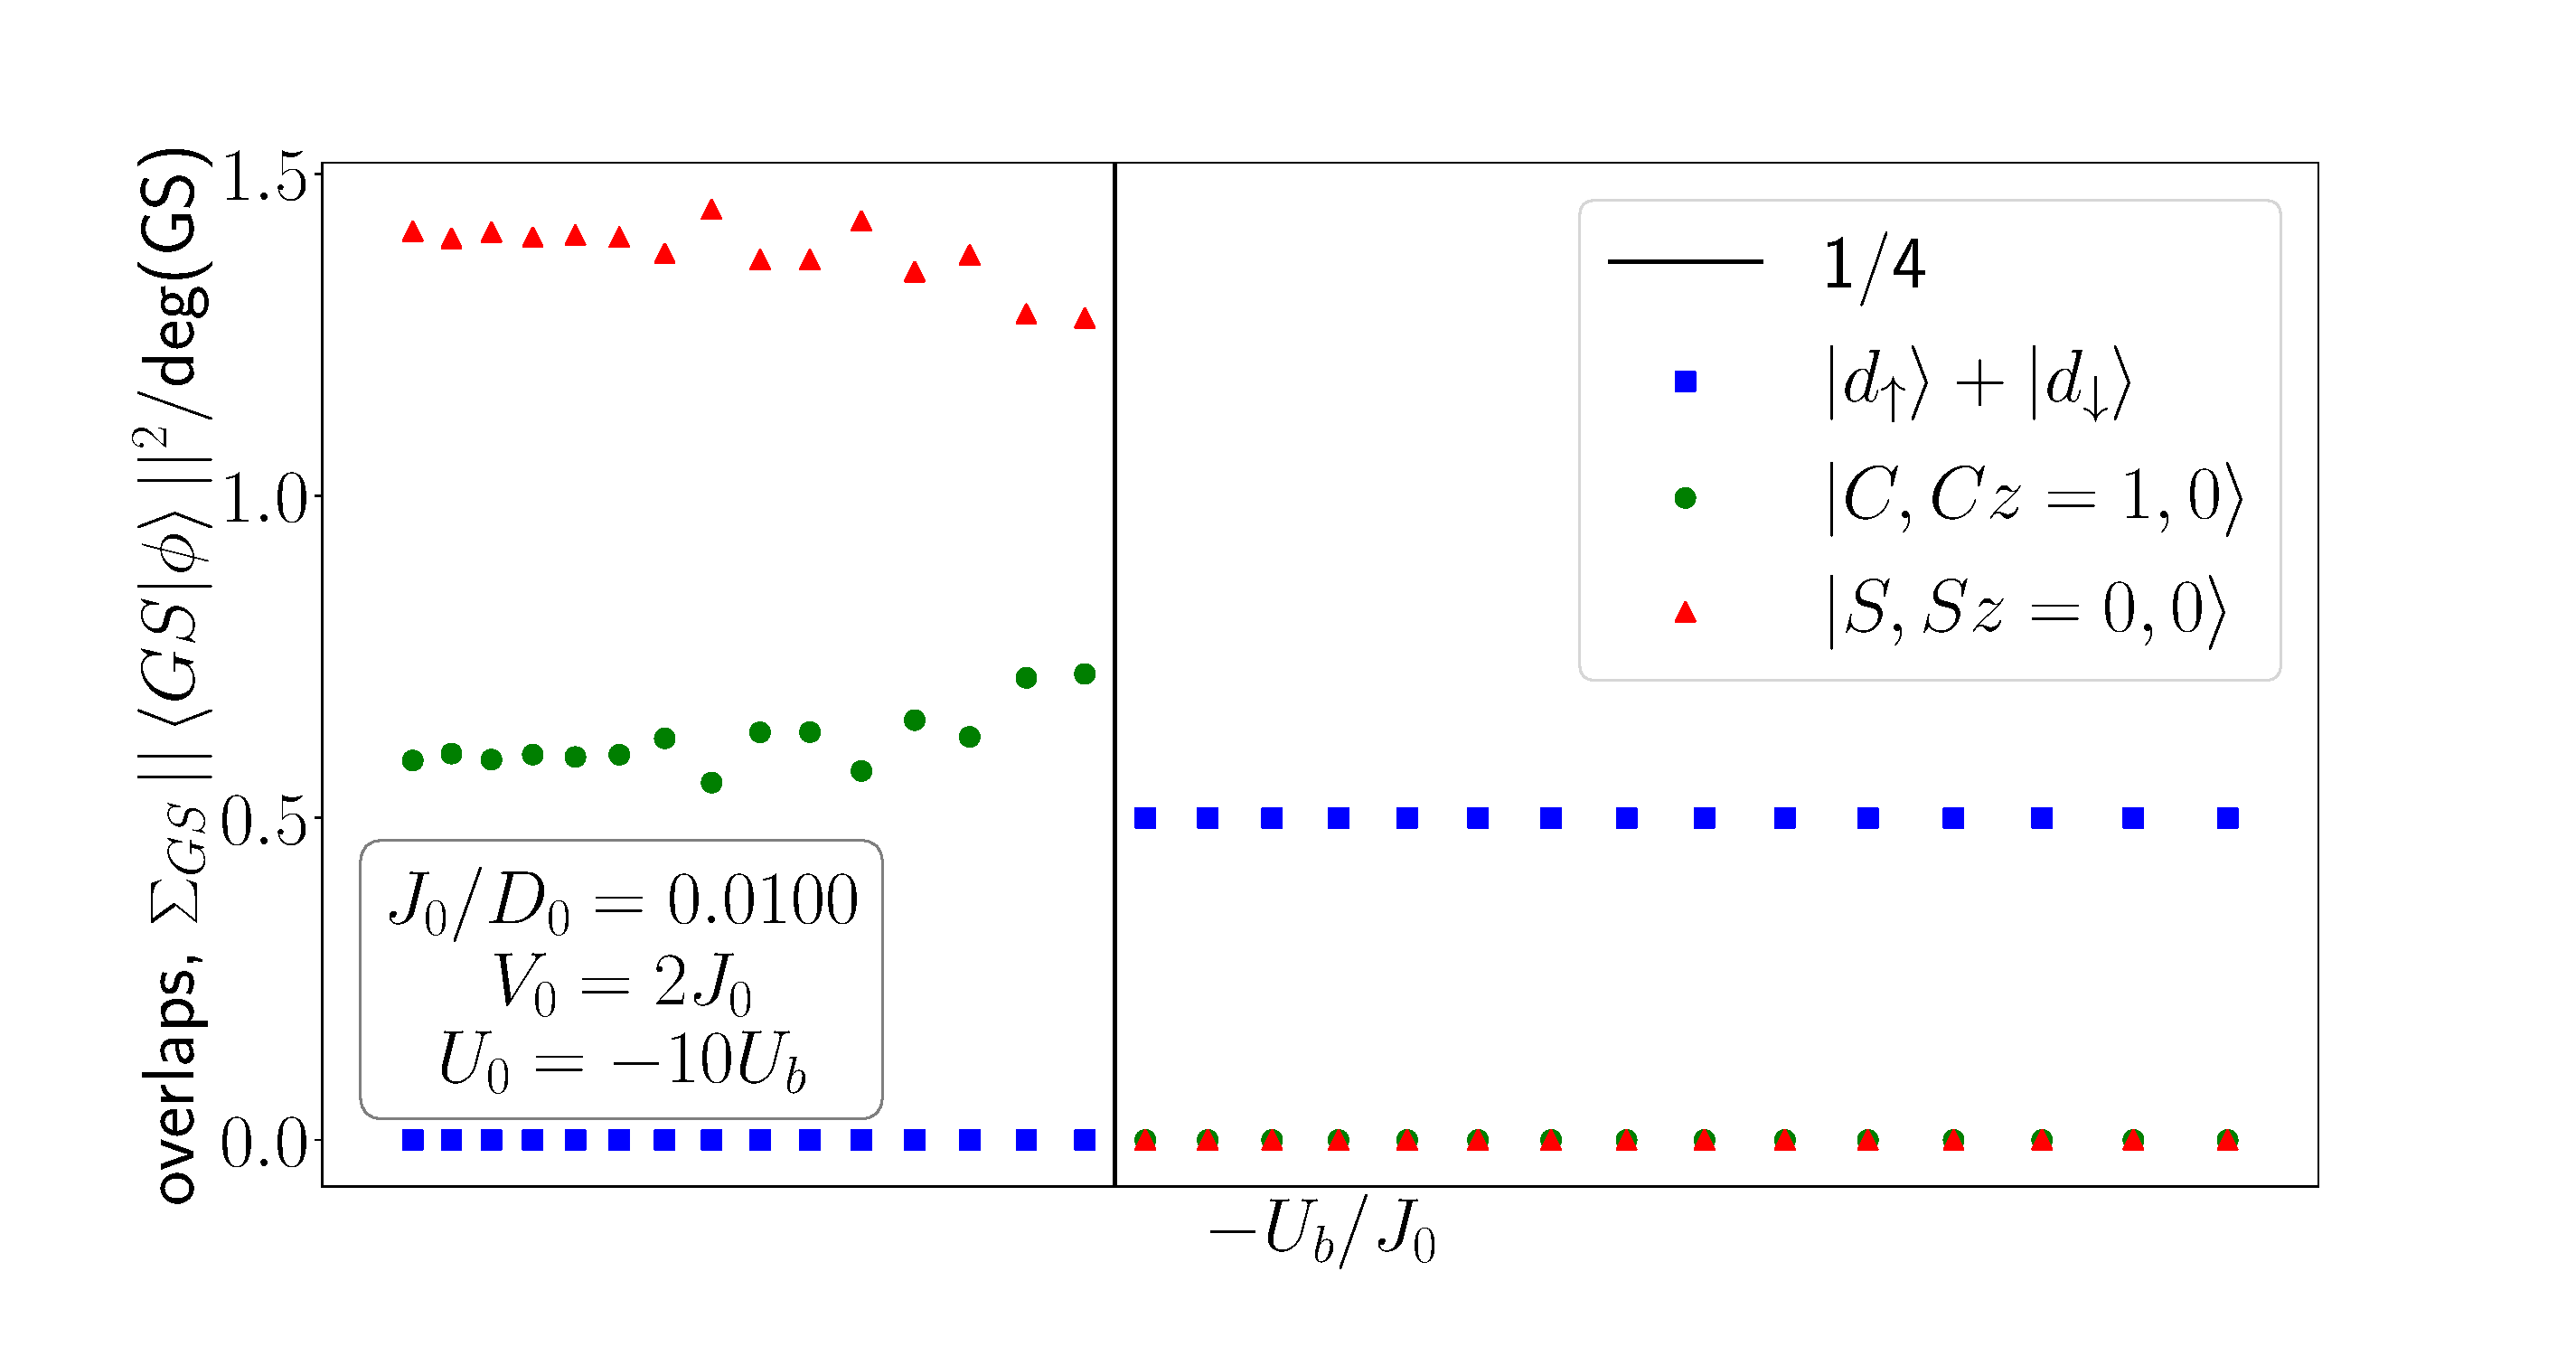
\includegraphics[width=0.7\textwidth]{../figures/overlaps_gs-J=10.000.pdf}\\
	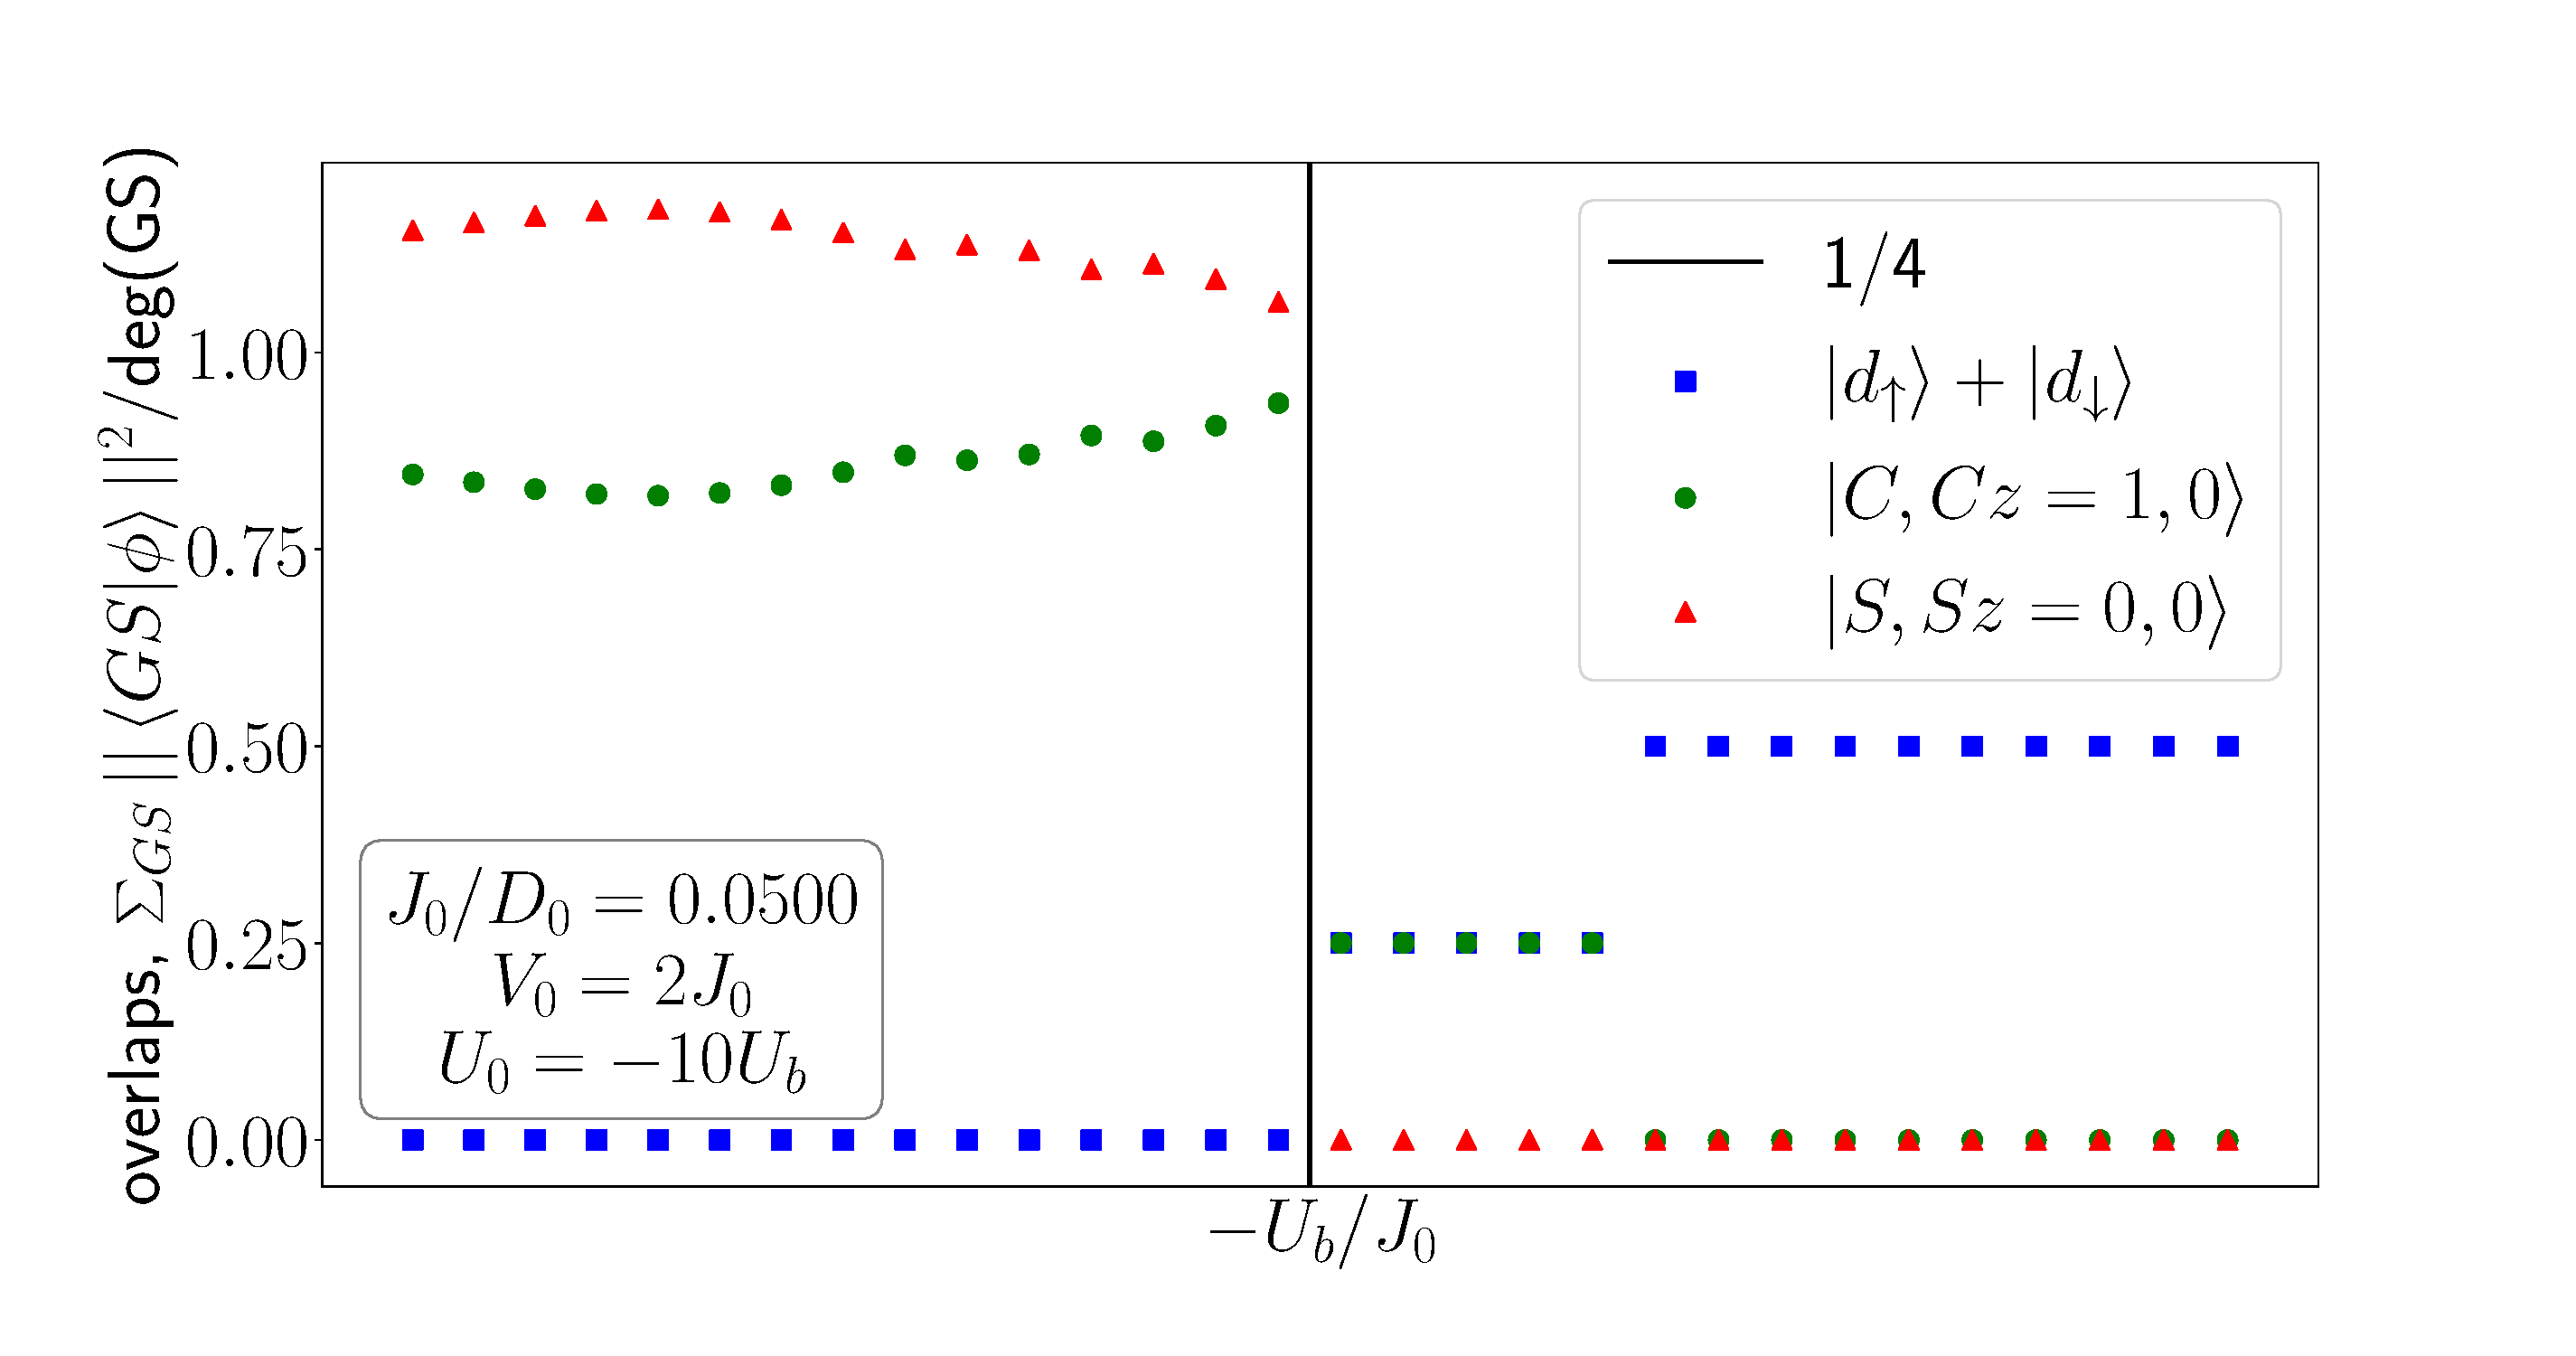
\includegraphics[width=0.7\textwidth]{../figures/overlaps_gs-J=50.000.pdf}
\end{center}

\subsection*{Spin and charge correlations in ground state}
\begin{center}
	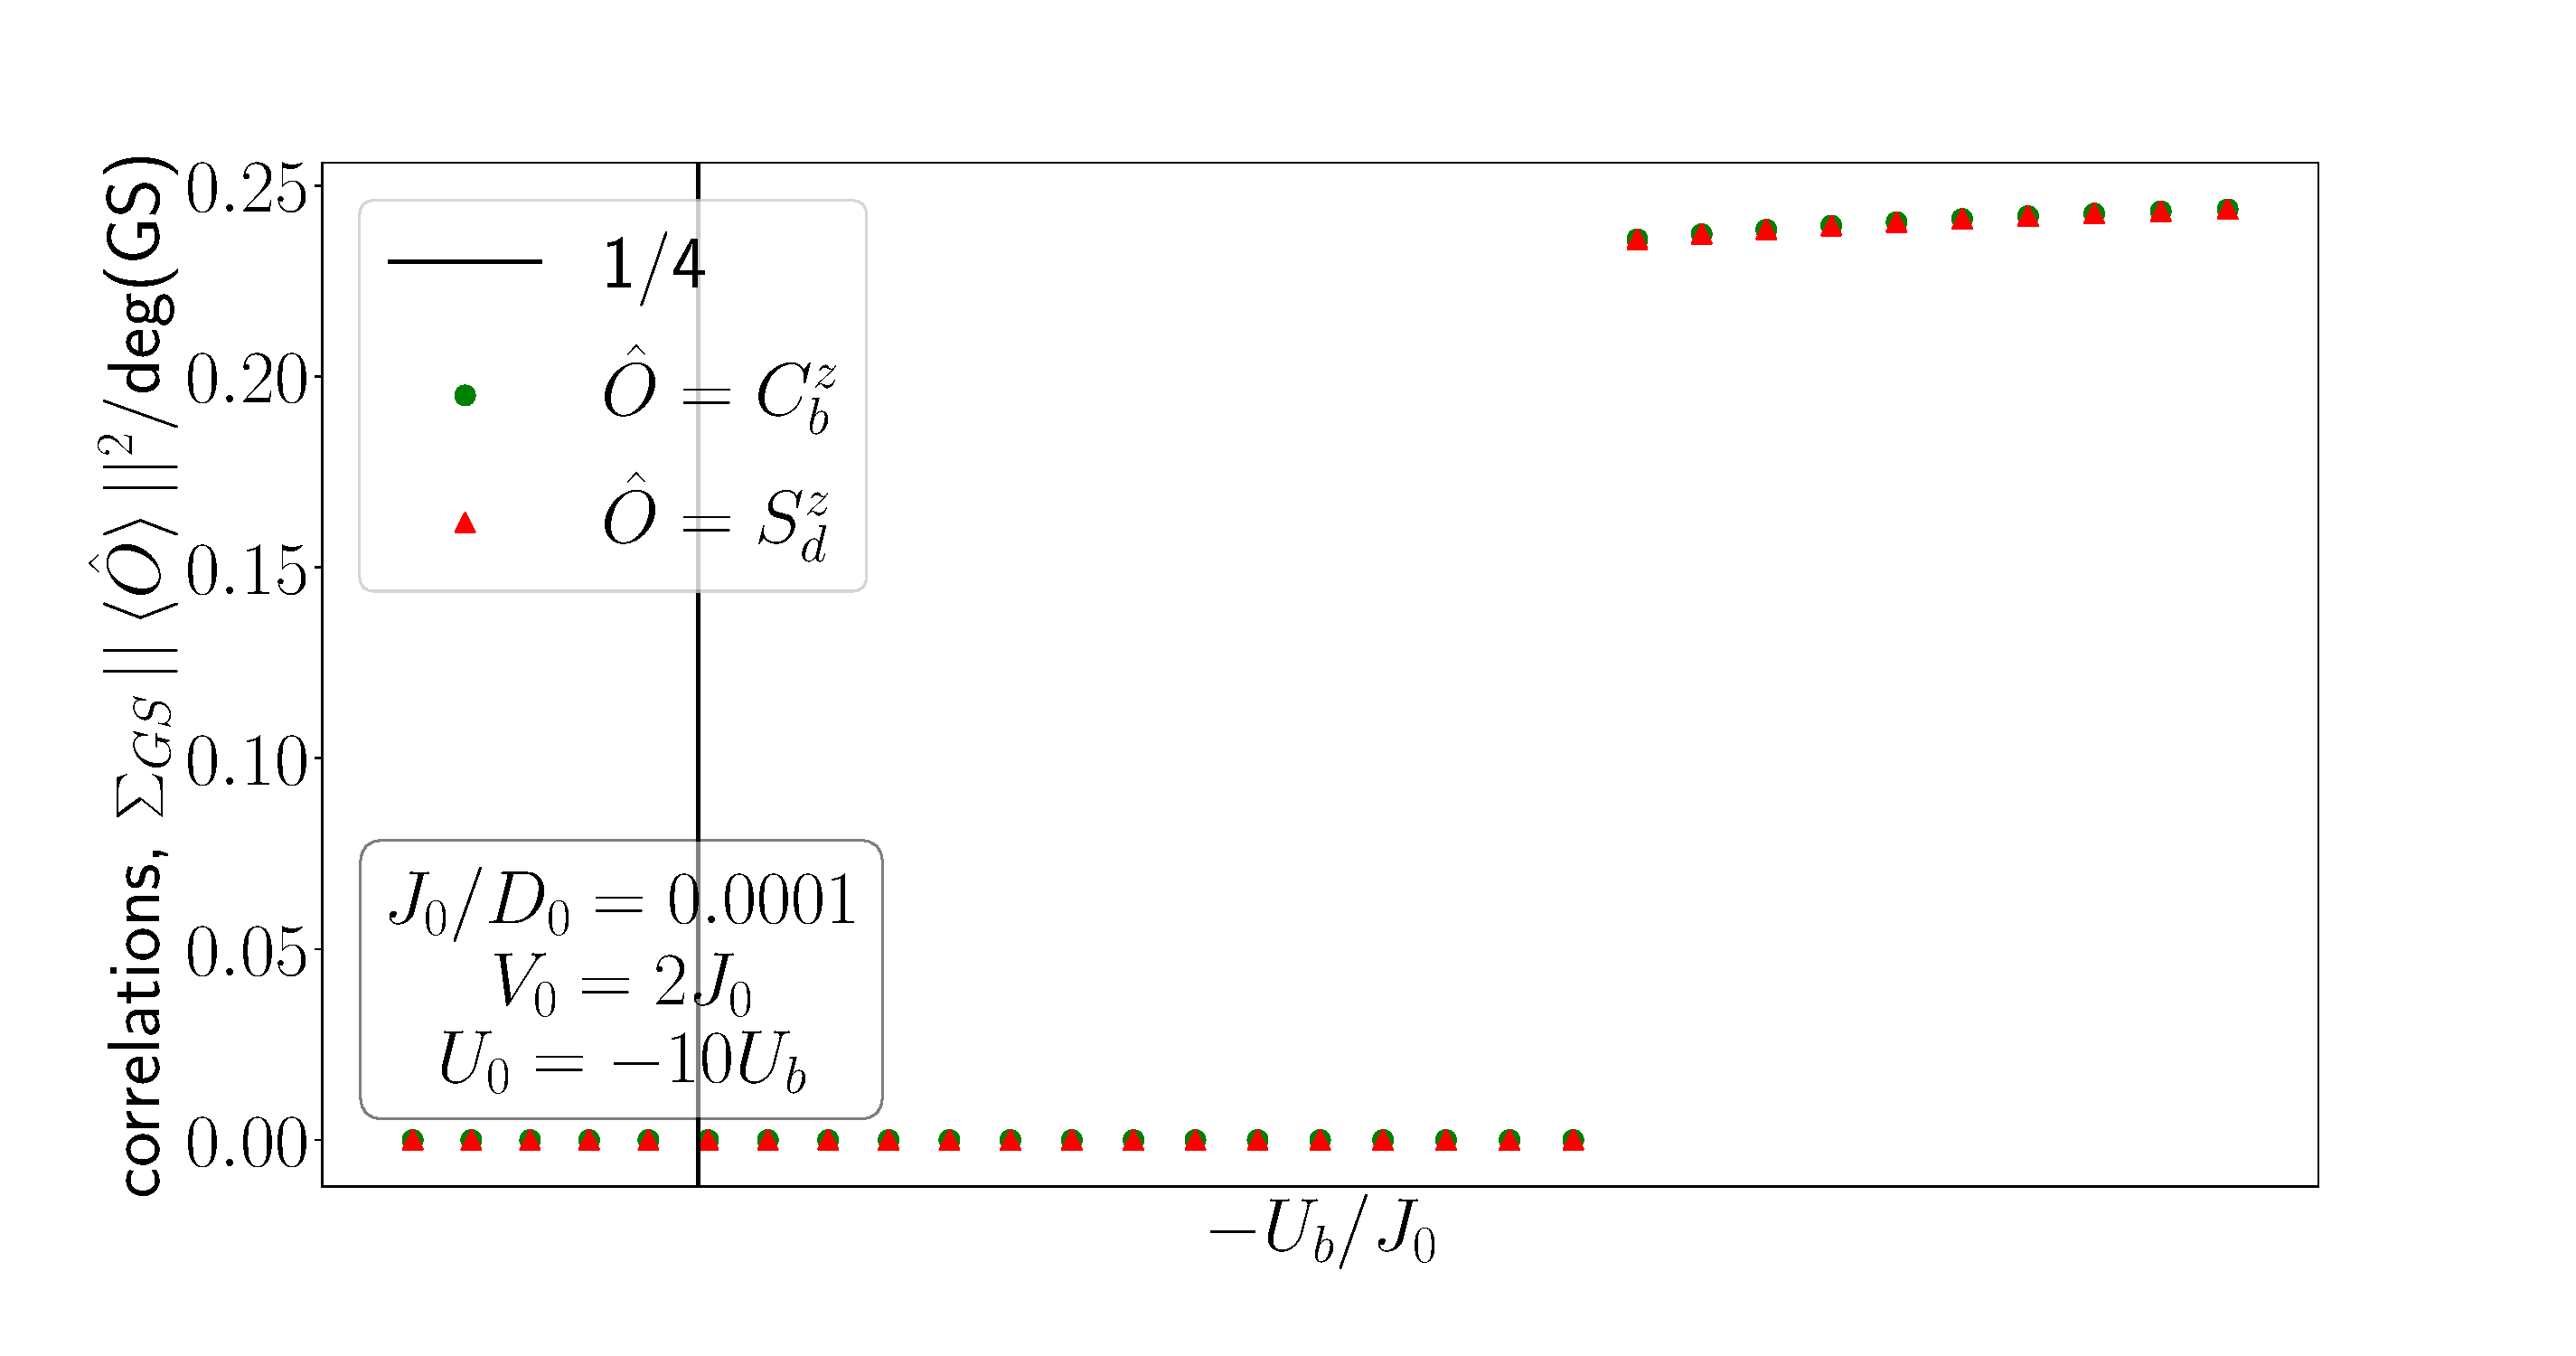
\includegraphics[width=0.7\textwidth]{../figures/corrs_gs-J=0.100.pdf}\\
	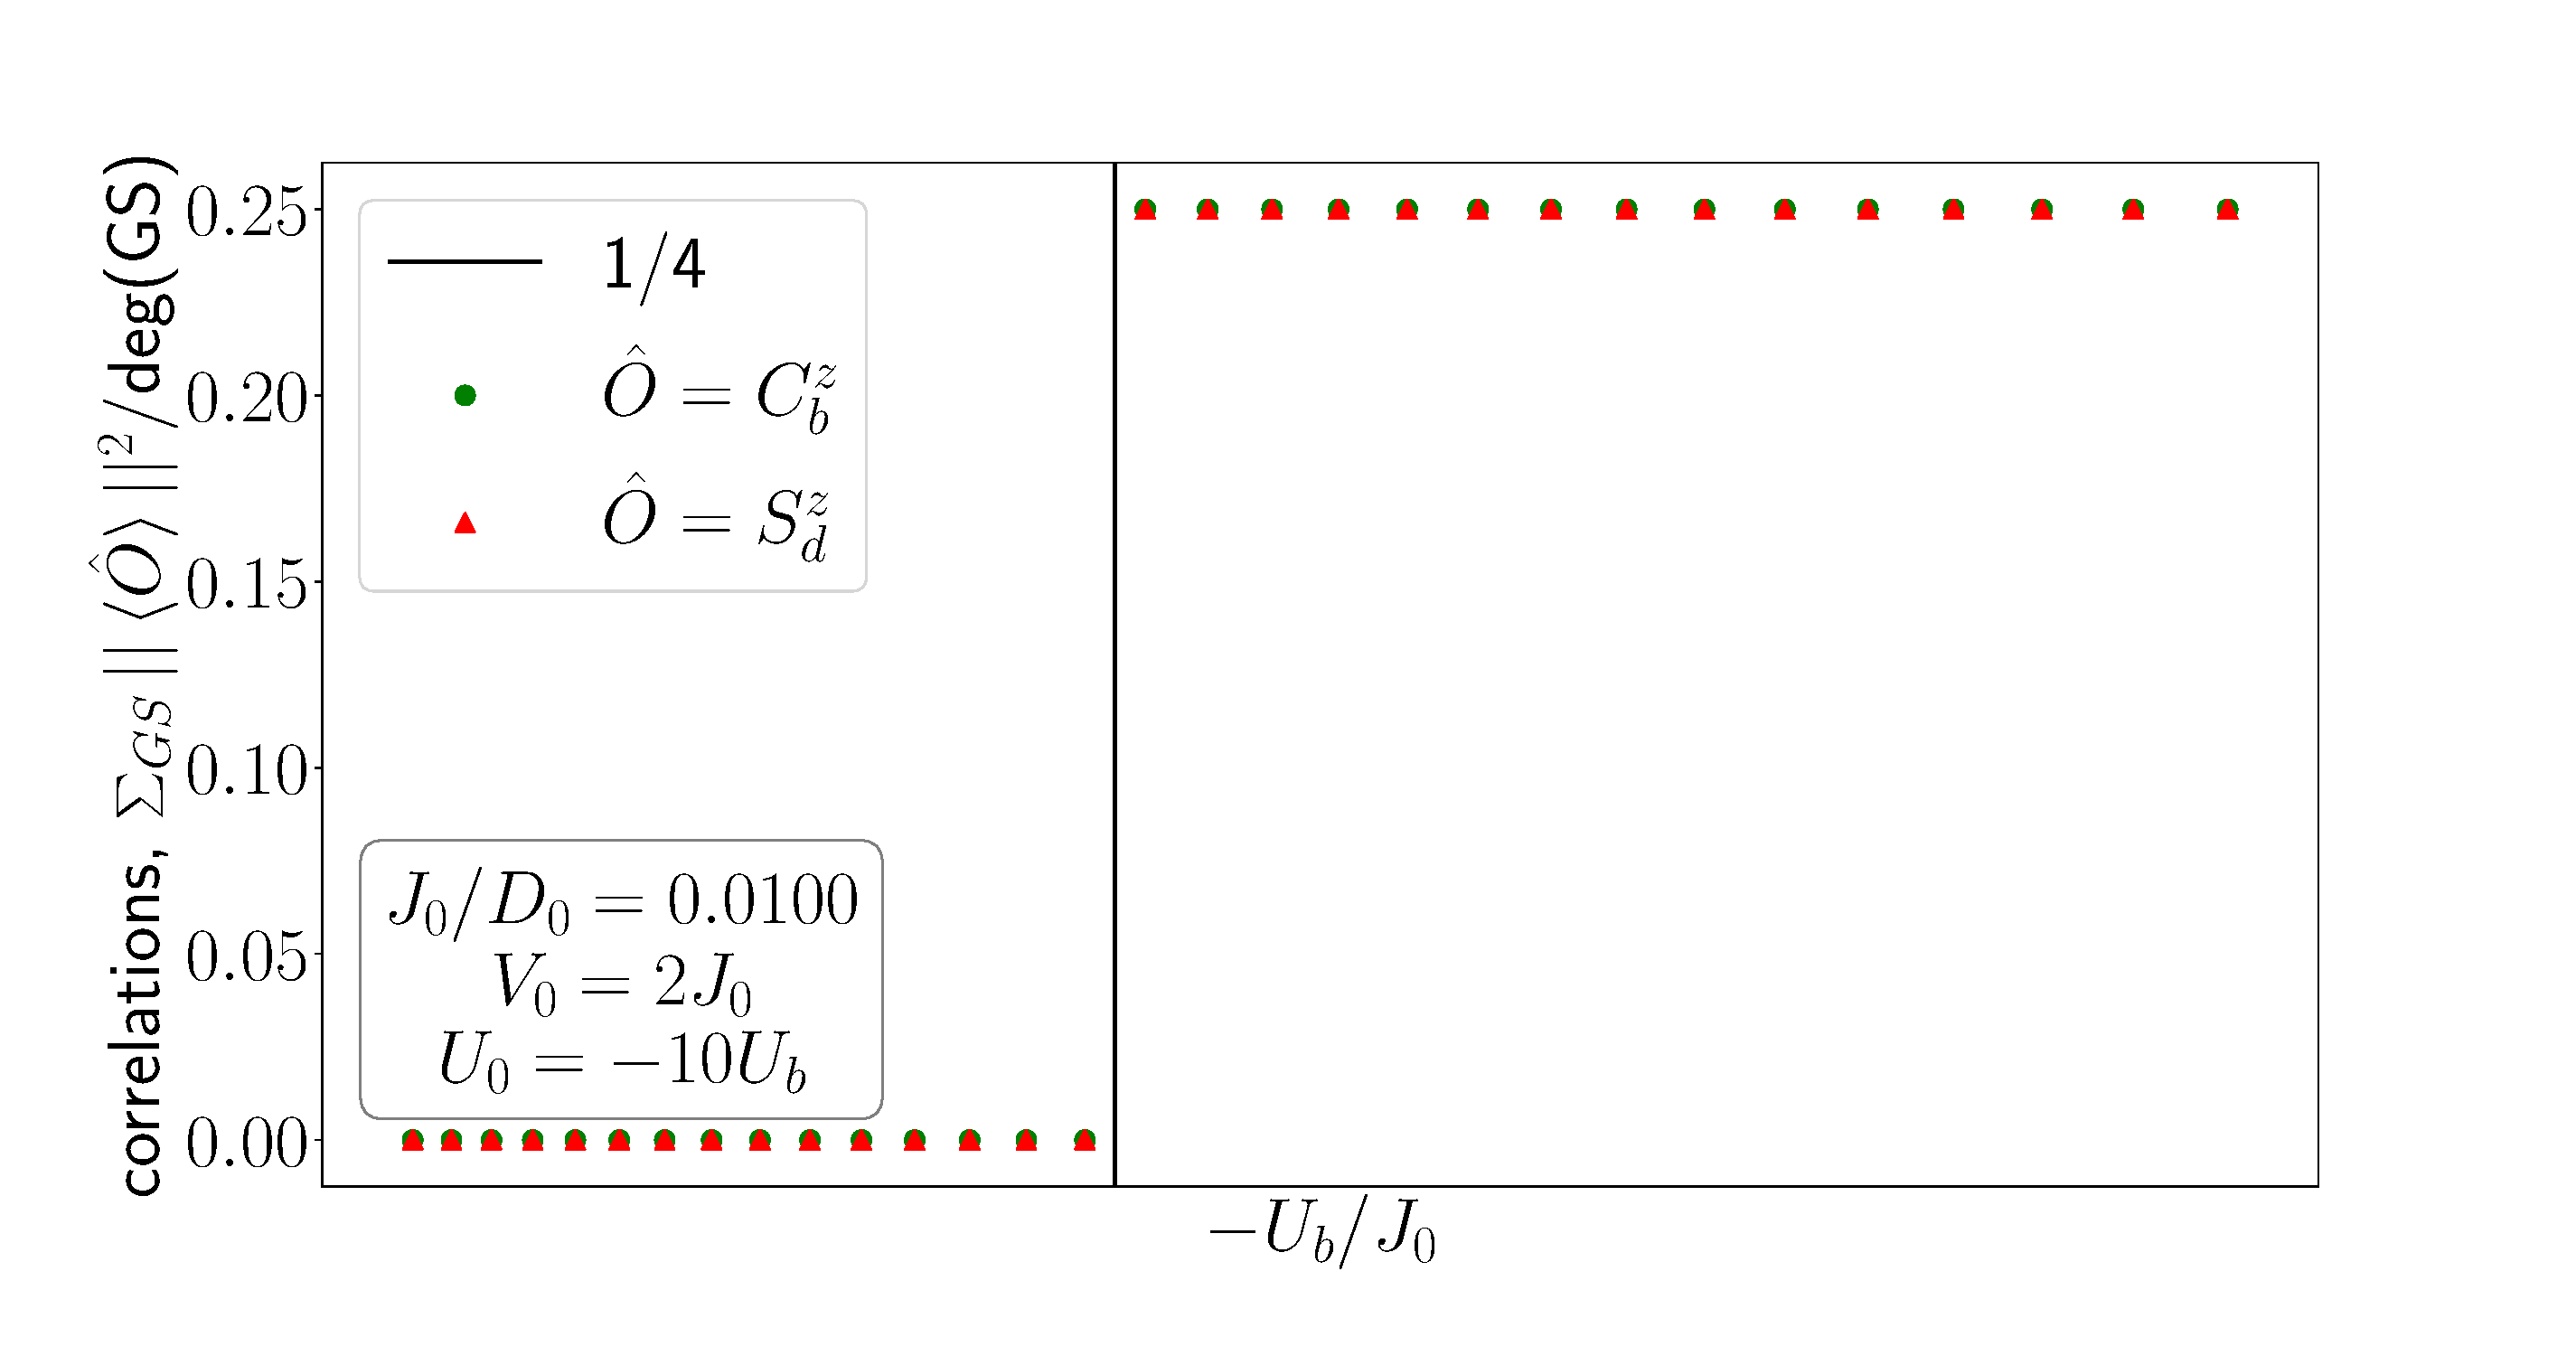
\includegraphics[width=0.7\textwidth]{../figures/corrs_gs-J=10.000.pdf}\\
	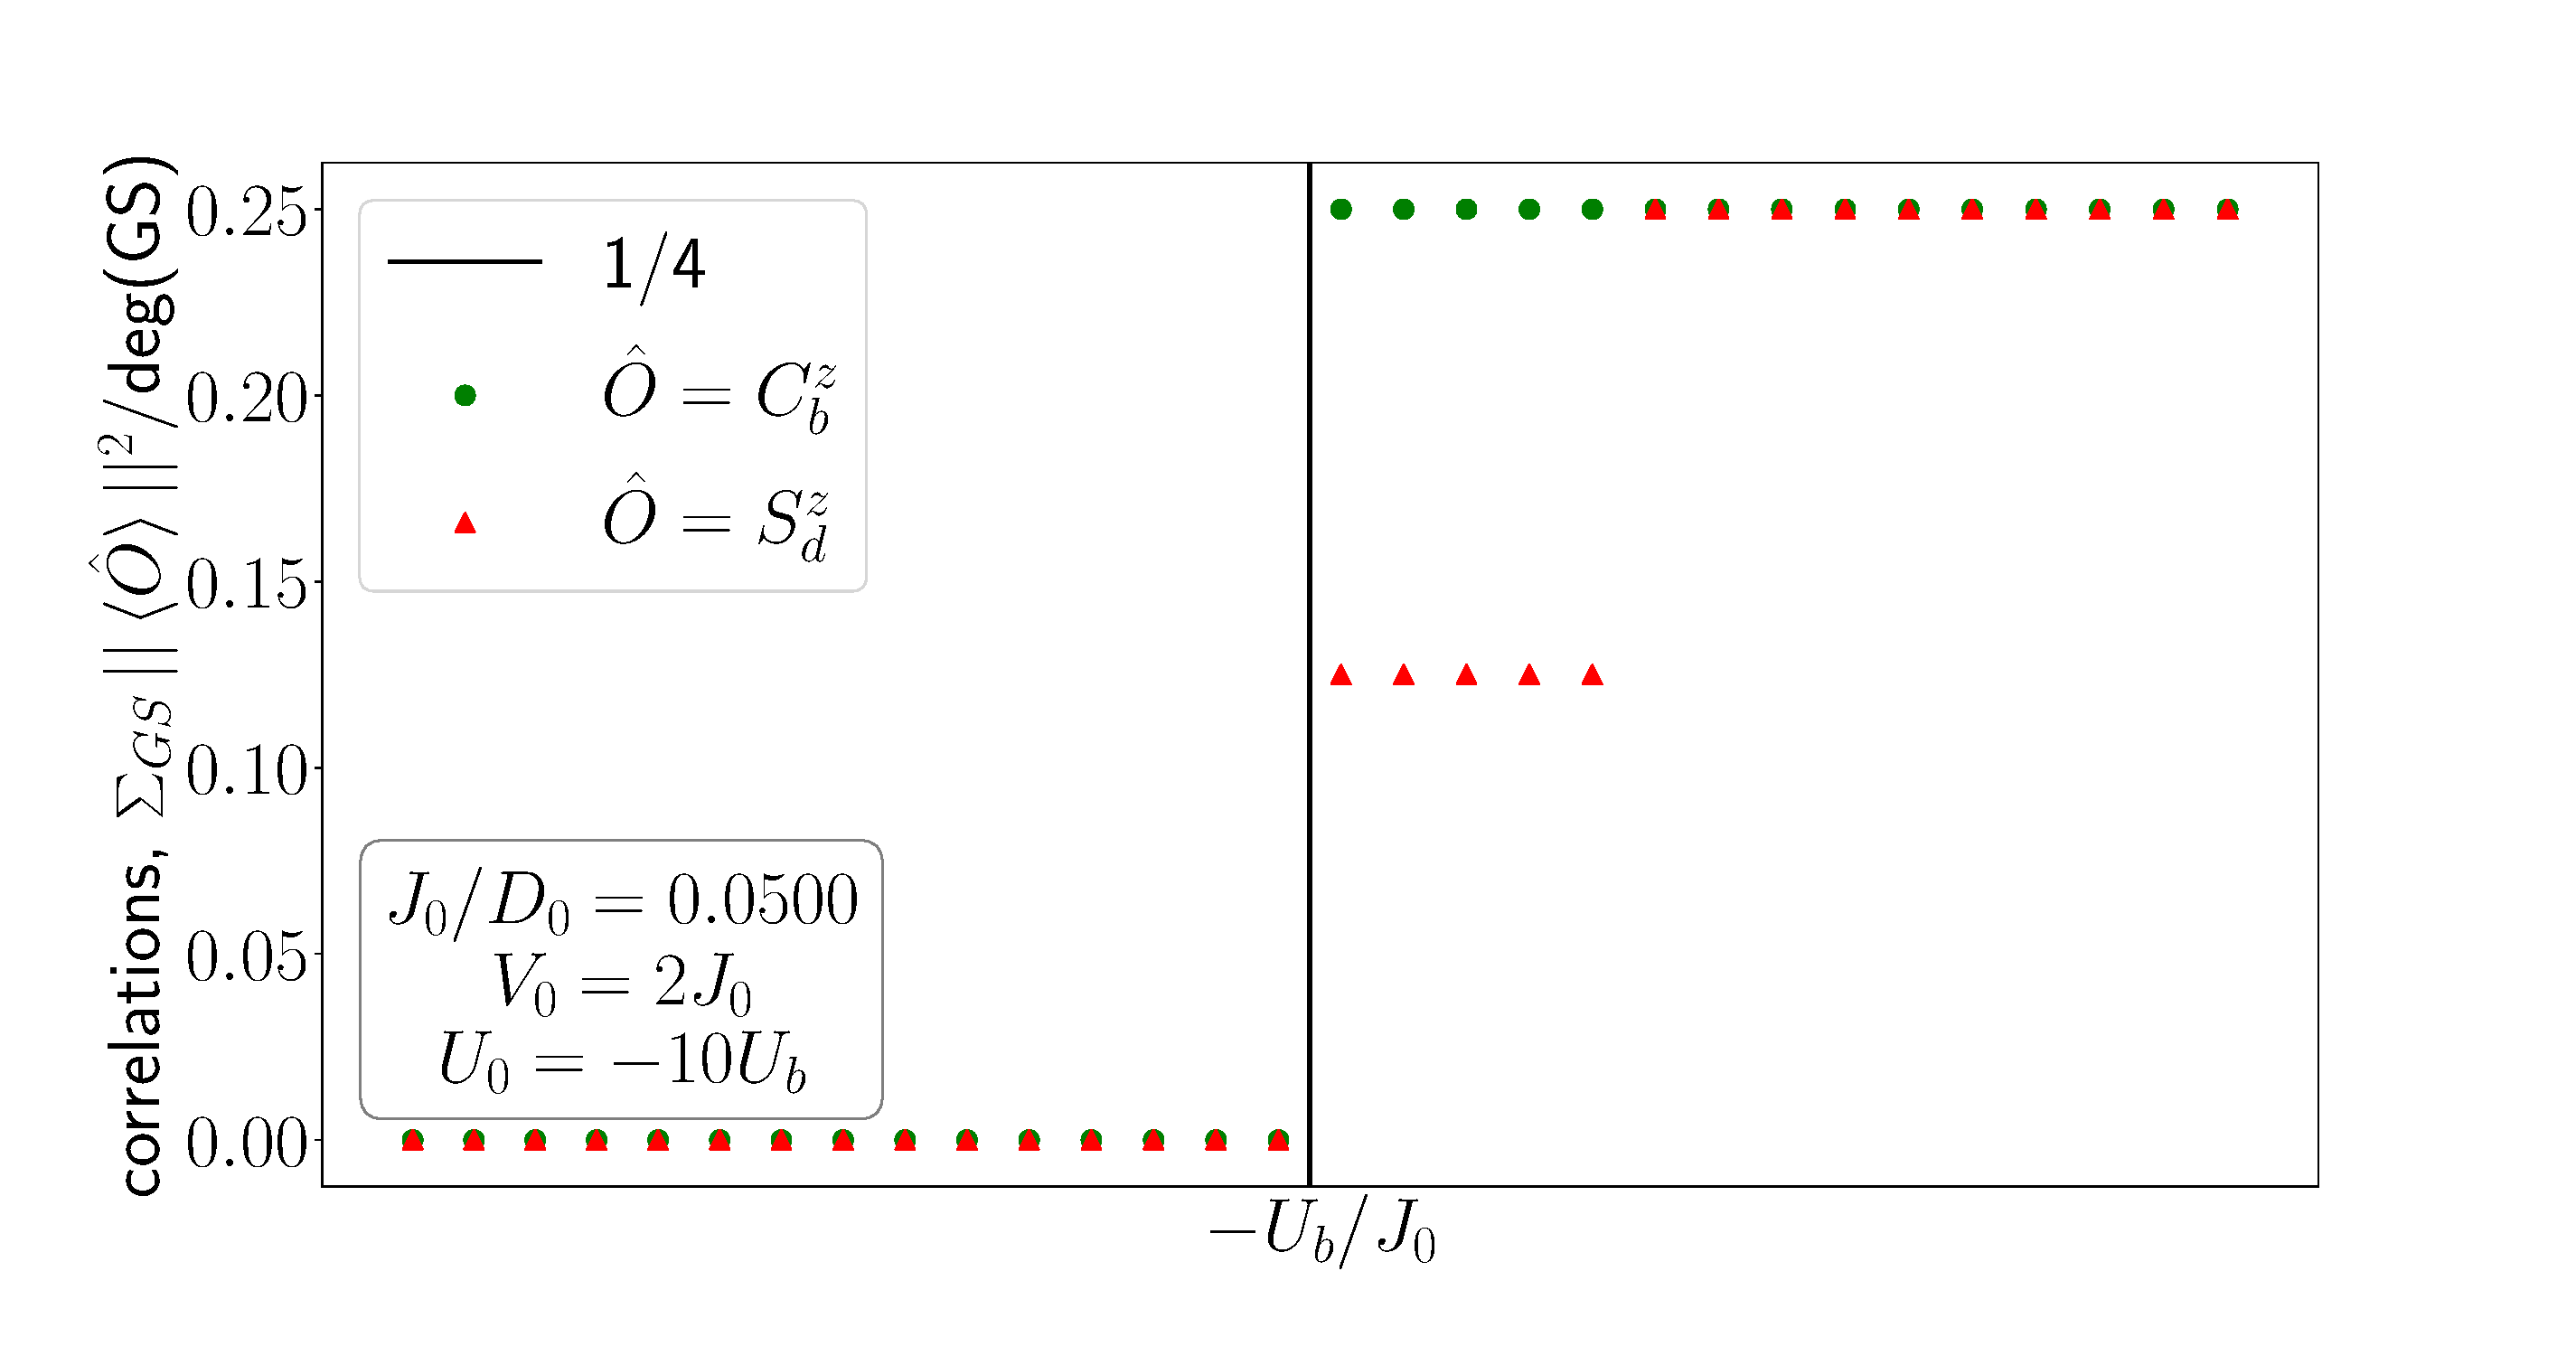
\includegraphics[width=0.7\textwidth]{../figures/corrs_gs-J=50.000.pdf}
\end{center}


\section{Evolution of various correlation measures and other quantities}

\subsection*{Perturbation theoretic terms}
These quantities are related to the local Fermi liquid of the Kondo strong coupling fixed point and the perturbation theory associated with it. \(min(\delta E)\) is the gap in the spectrum of the two-site Hamiltonian; this which acts as the denominator for the perturbation theoretic calculations. \(t^2/\delta E\) is the small parameter for the expansion, \(t\) being the tight-binding hopping. 
\begin{center}
	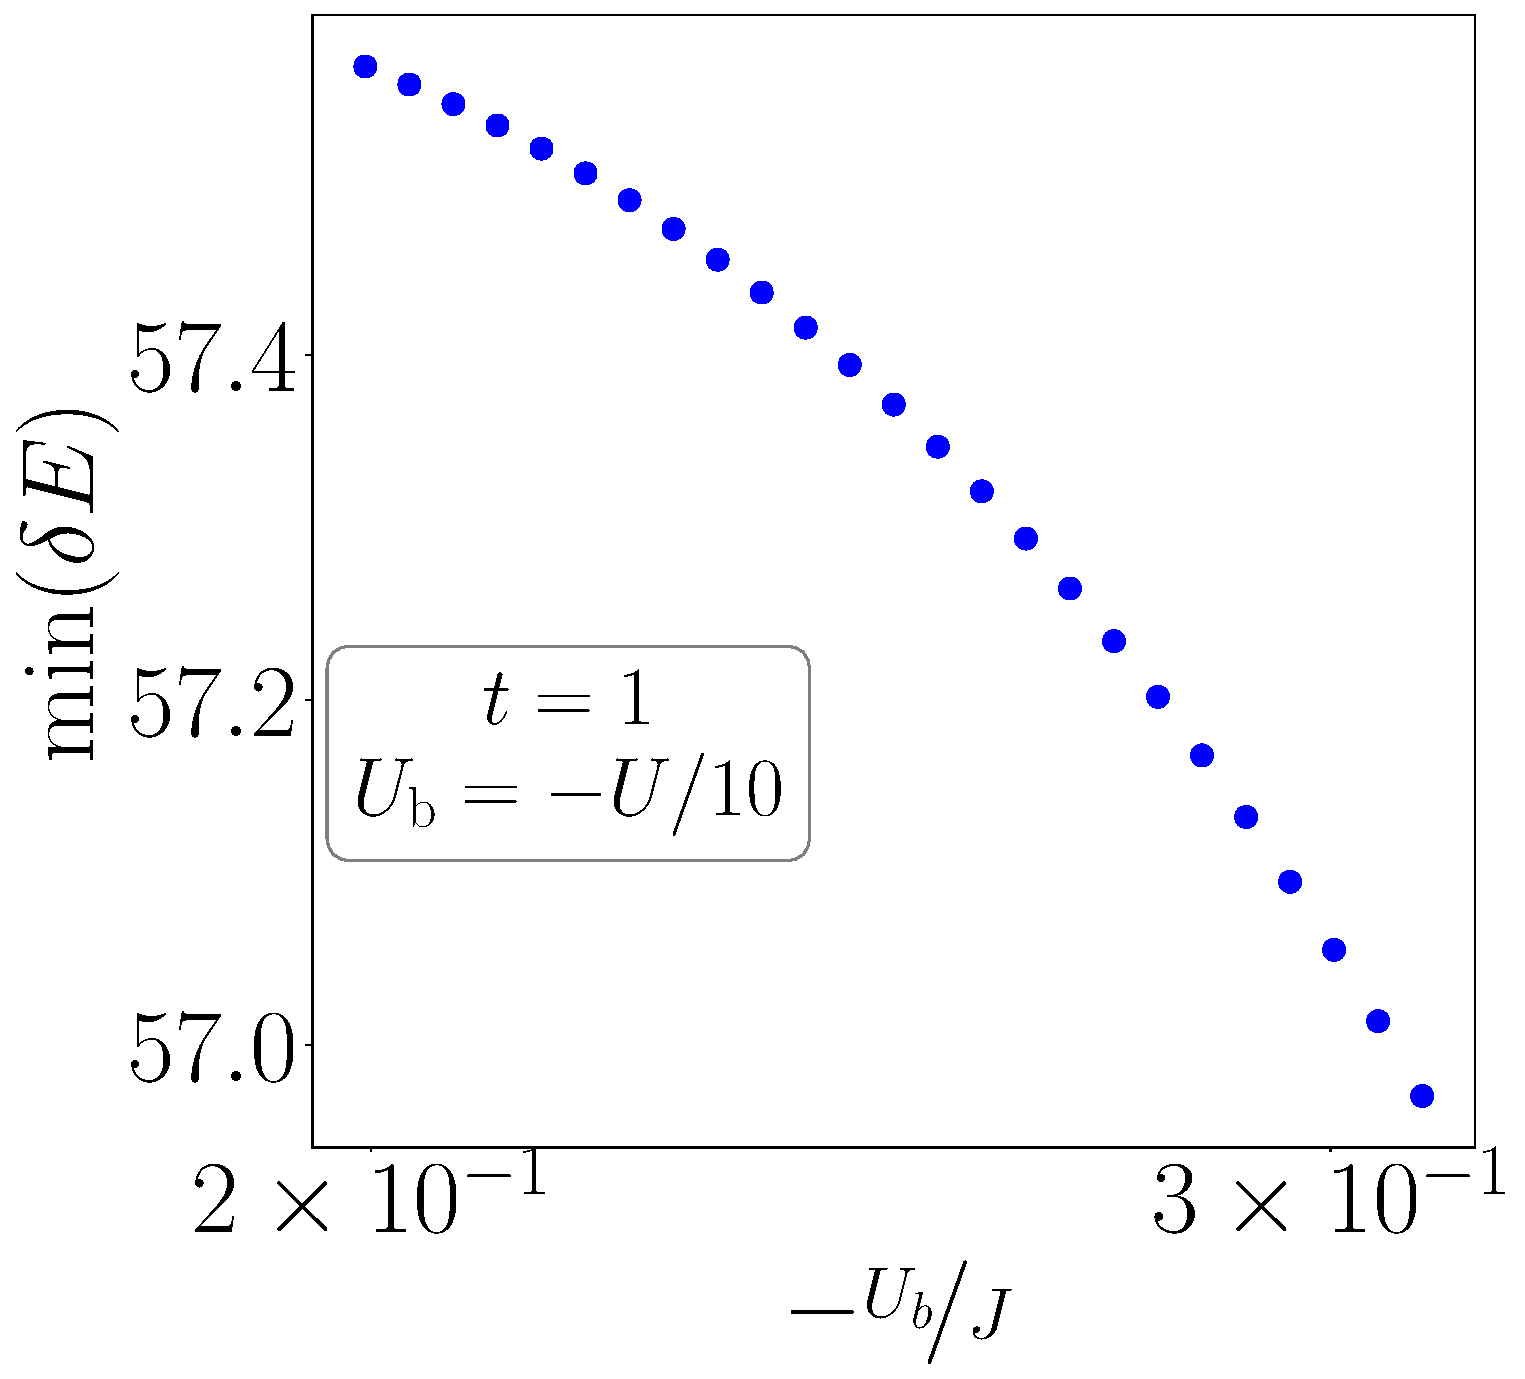
\includegraphics[width=0.32\textwidth]{../figures/gap-D=1000.00000,t=1.00000,J=30.00000,V=1.50000J,Ub=-Uby10,N=4,U=59.85787,93.55363,25.pdf}
	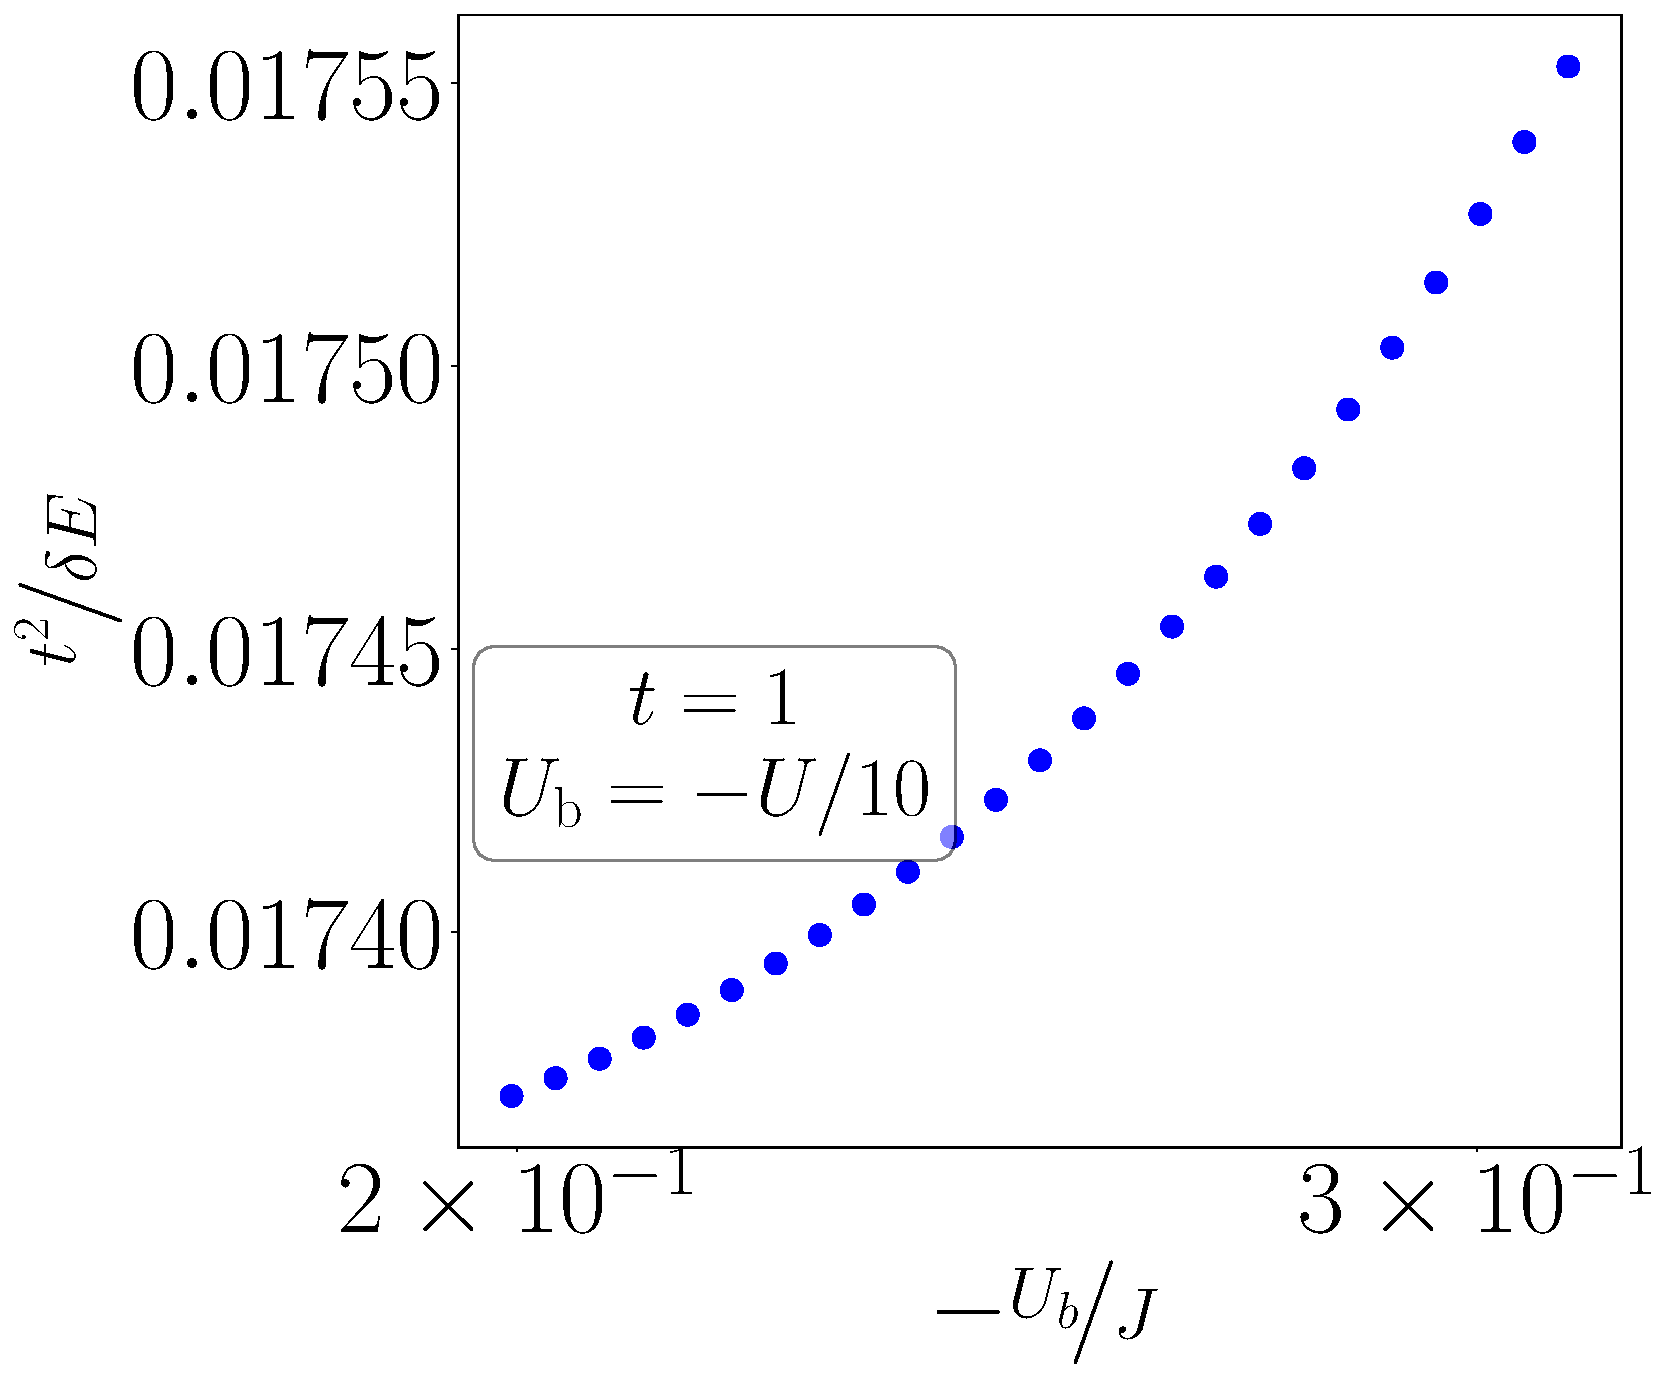
\includegraphics[width=0.32\textwidth]{../figures/par-D=1000.00000,t=1.00000,J=30.00000,V=1.50000J,Ub=-Uby10,N=4,U=59.85787,93.55363,25.pdf}
\end{center}

\subsection*{Correlation within the Kondo cloud}
\begin{center}
	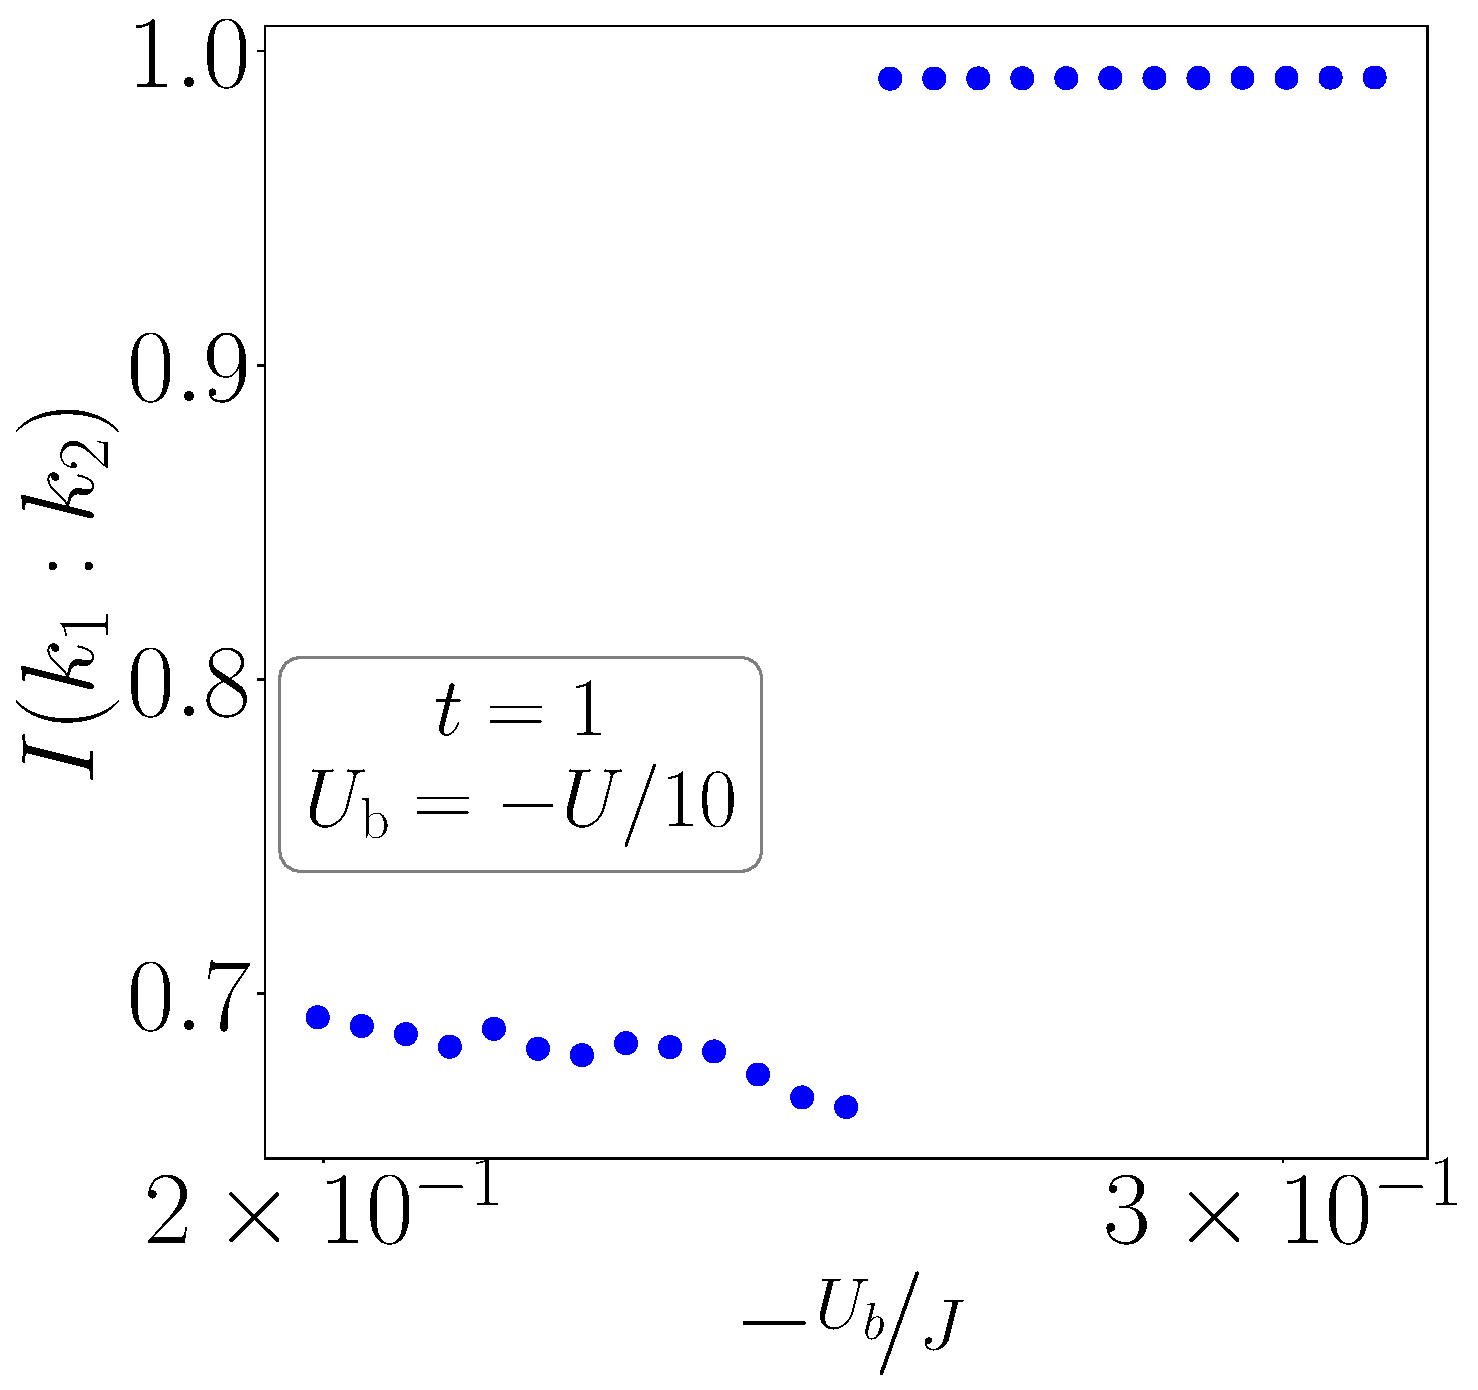
\includegraphics[width=0.32\textwidth]{../figures/corr-k-D=1000.00000,t=1.00000,J=30.00000,V=1.50000J,Ub=-Uby10,N=4,U=59.85787,93.55363,25.pdf}
	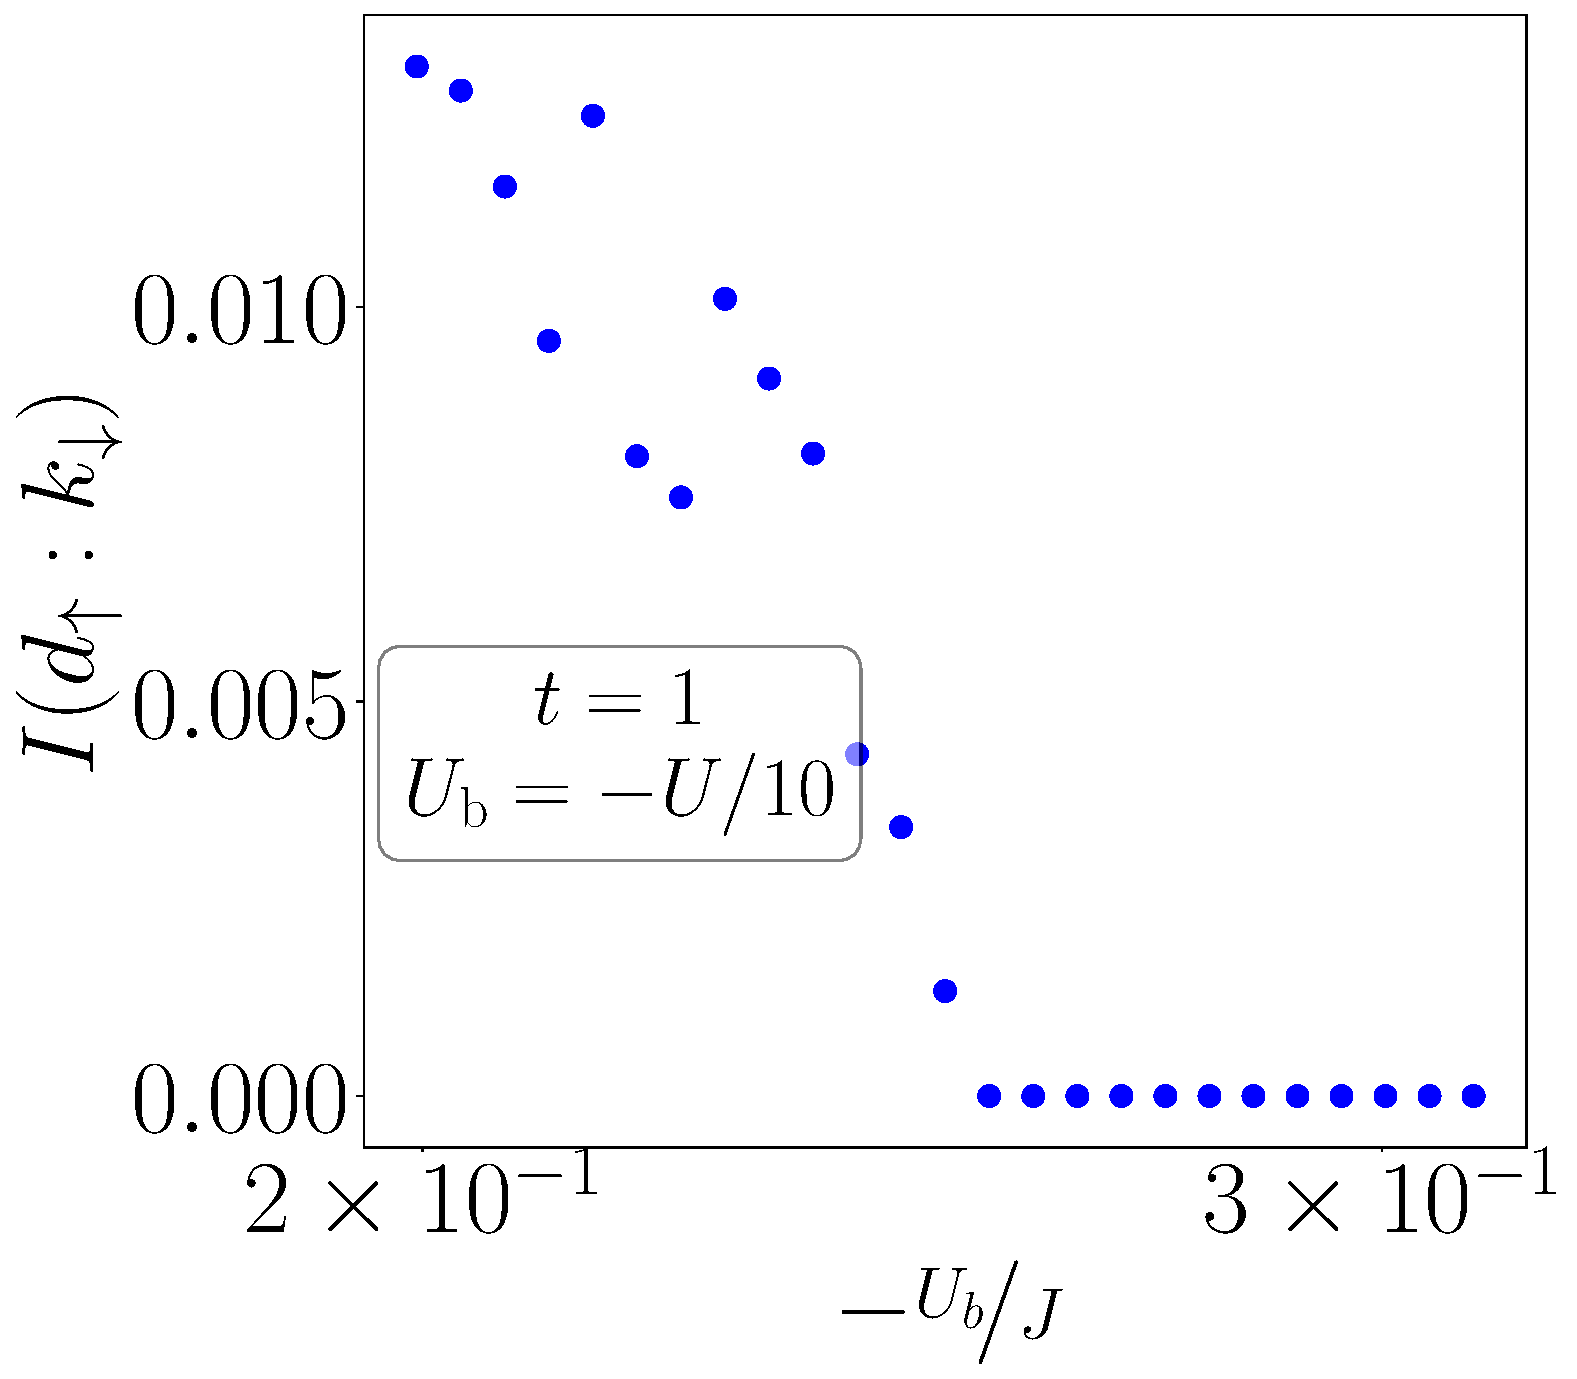
\includegraphics[width=0.32\textwidth]{../figures/mi-dk-D=1000.00000,t=1.00000,J=30.00000,V=1.50000J,Ub=-Uby10,N=4,U=59.85787,93.55363,25.pdf}
	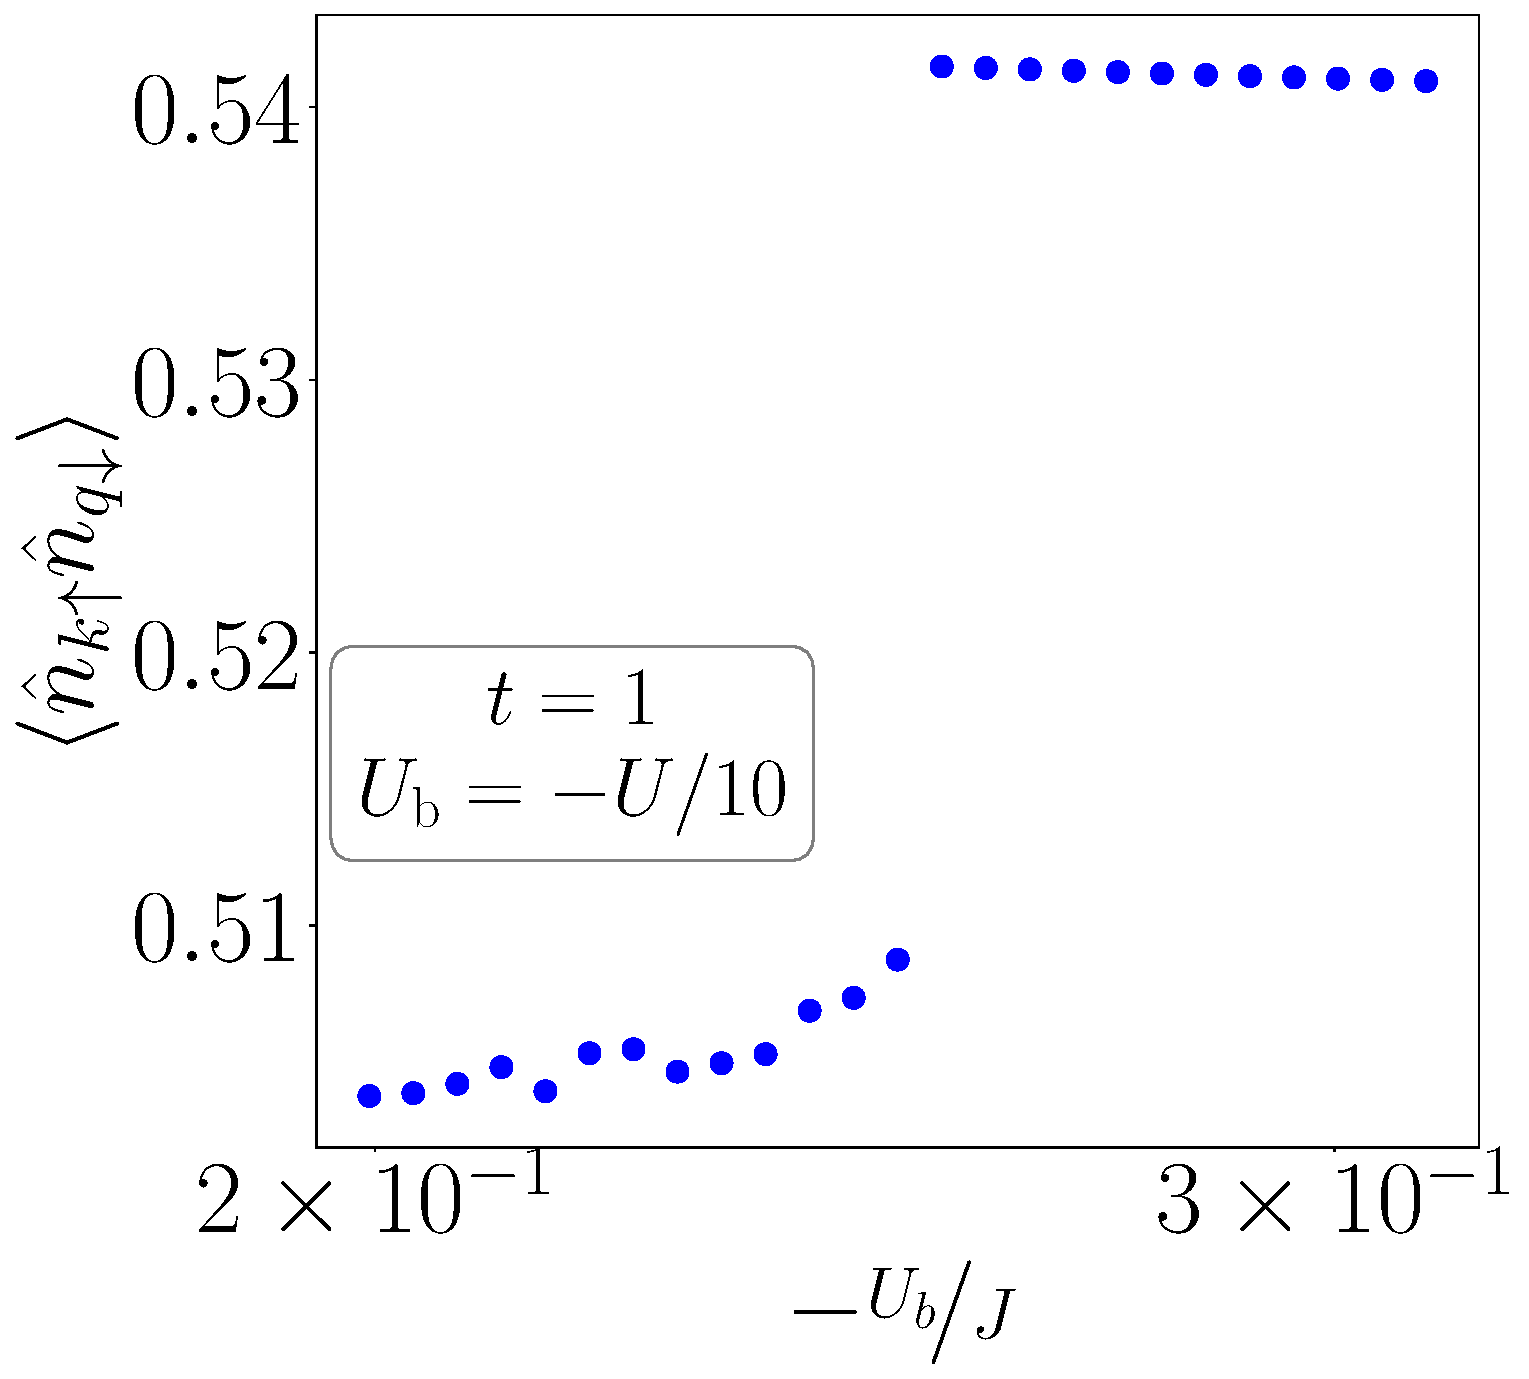
\includegraphics[width=0.32\textwidth]{../figures/corr-k-diag-D=1000.00000,t=1.00000,J=30.00000,V=1.50000J,Ub=-Uby10,N=4,U=59.85787,93.55363,25.pdf}
	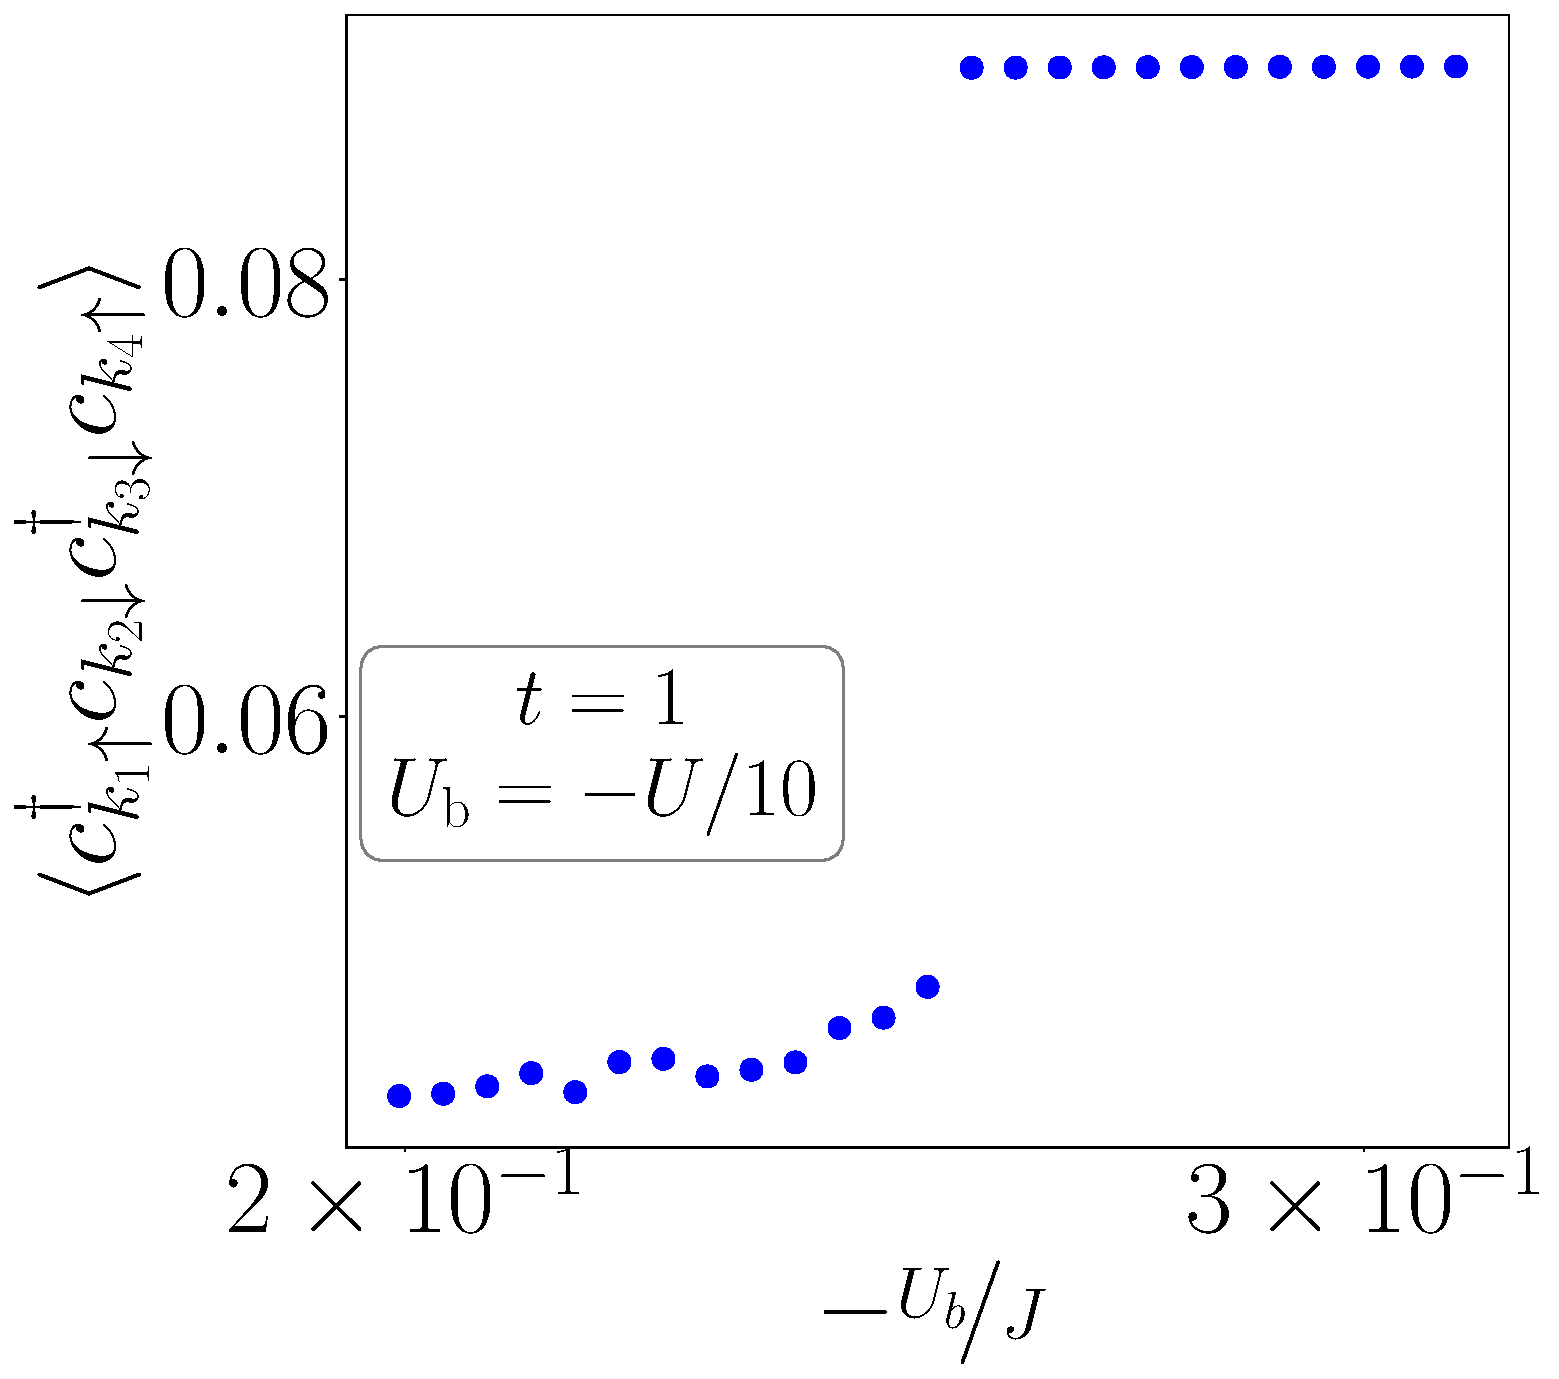
\includegraphics[width=0.32\textwidth]{../figures/corr-k-od-D=1000.00000,t=1.00000,J=30.00000,V=1.50000J,Ub=-Uby10,N=4,U=59.85787,93.55363,25.pdf}
\end{center}

\subsection*{Mutual information between various real space members}
\begin{center}
	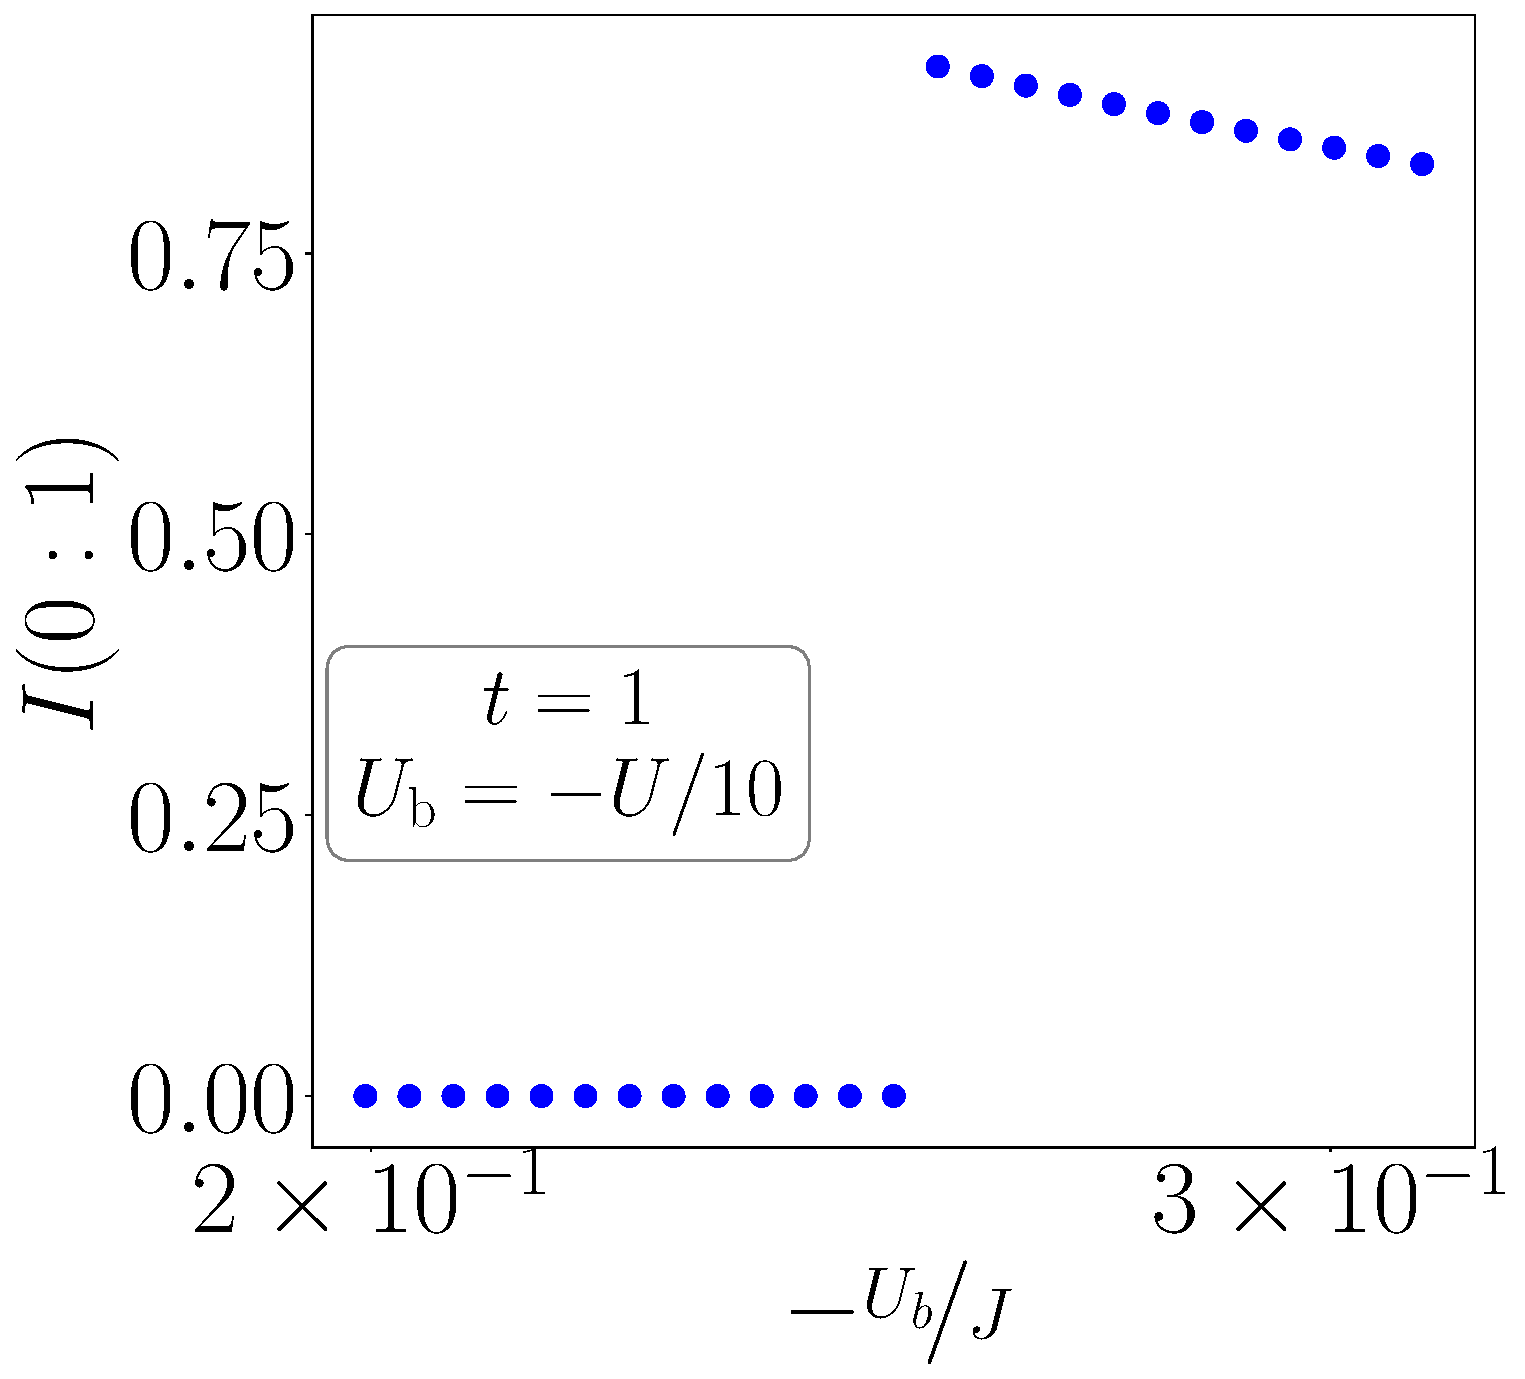
\includegraphics[width=0.32\textwidth]{../figures/mi-01-D=1000.00000,t=1.00000,J=30.00000,V=1.50000J,Ub=-Uby10,N=4,U=59.85787,93.55363,25.pdf}
	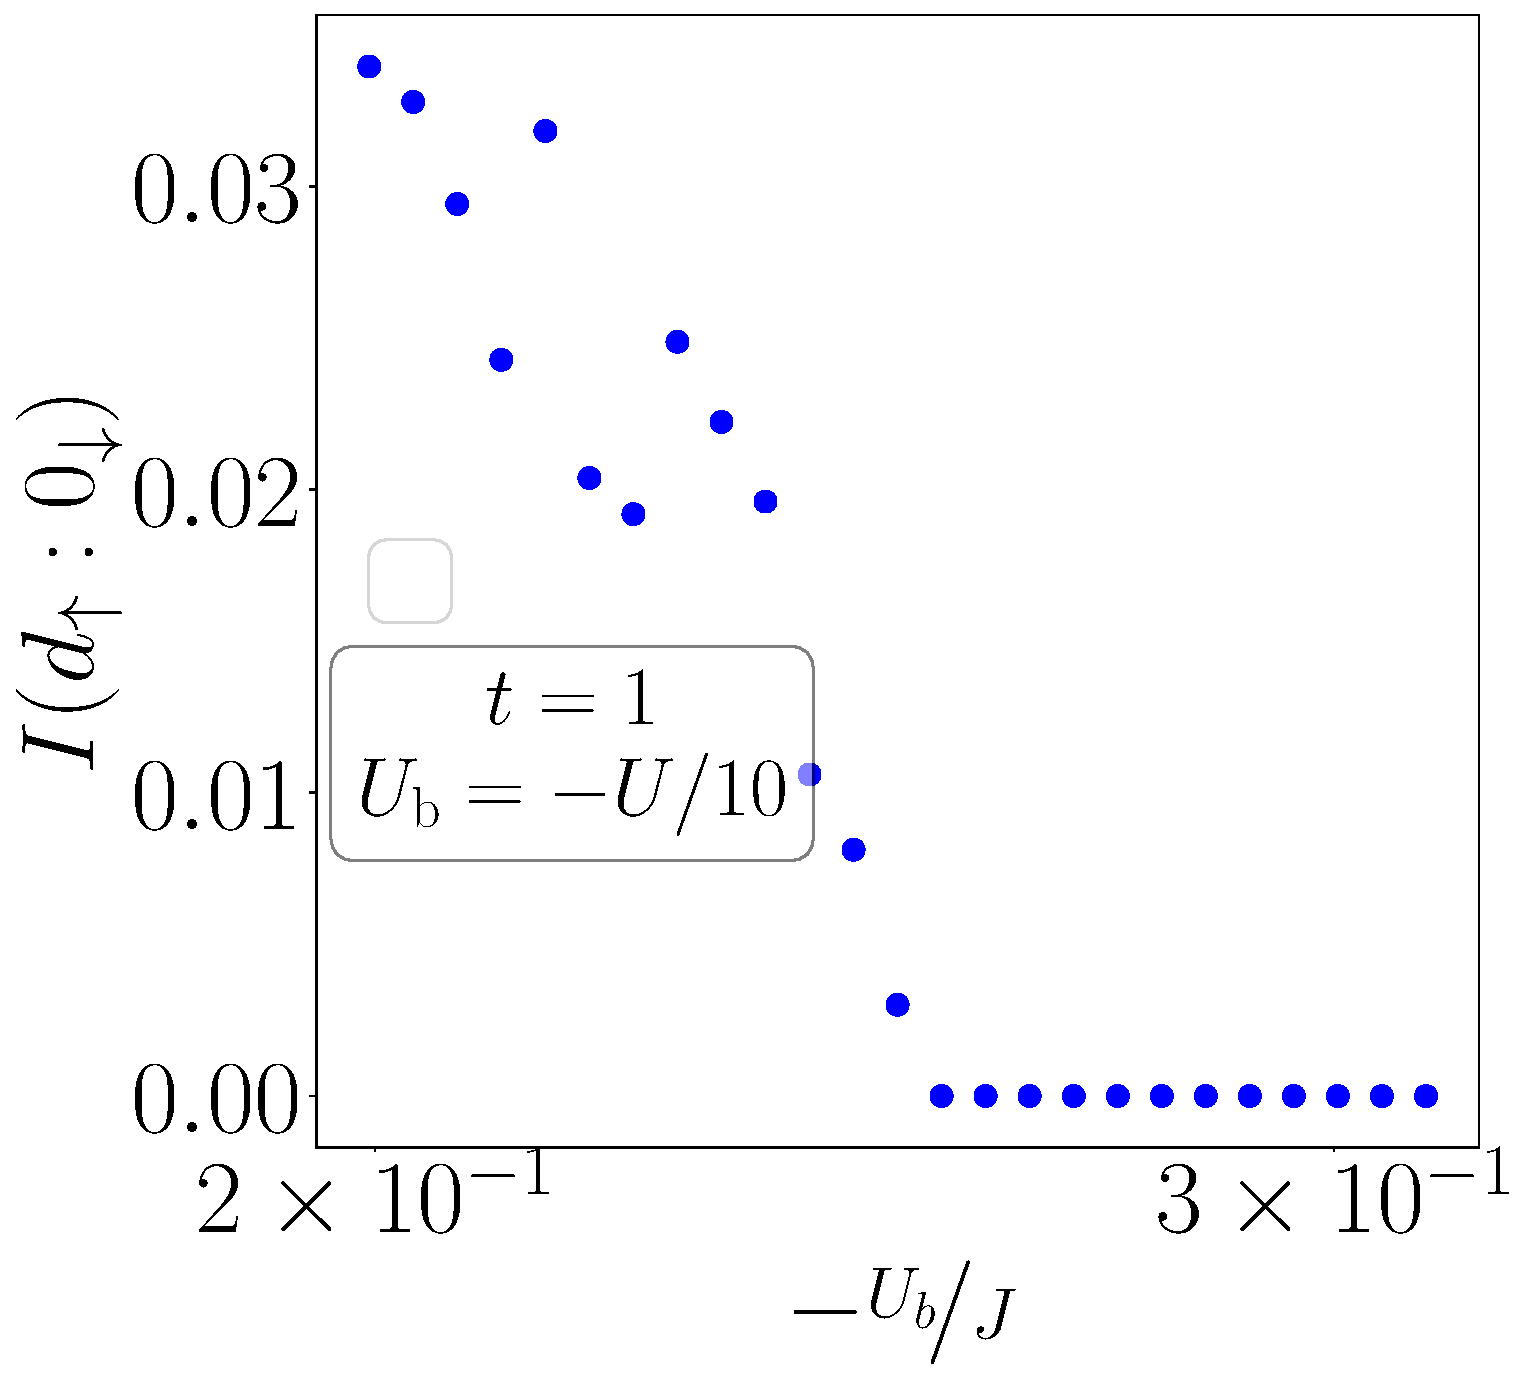
\includegraphics[width=0.32\textwidth]{../figures/mi-d0-D=1000.00000,t=1.00000,J=30.00000,V=1.50000J,Ub=-Uby10,N=4,U=59.85787,93.55363,25.pdf}
\end{center}

\subsection*{Impurity entanglement entropy and spin-spin correlations}

\begin{center}
	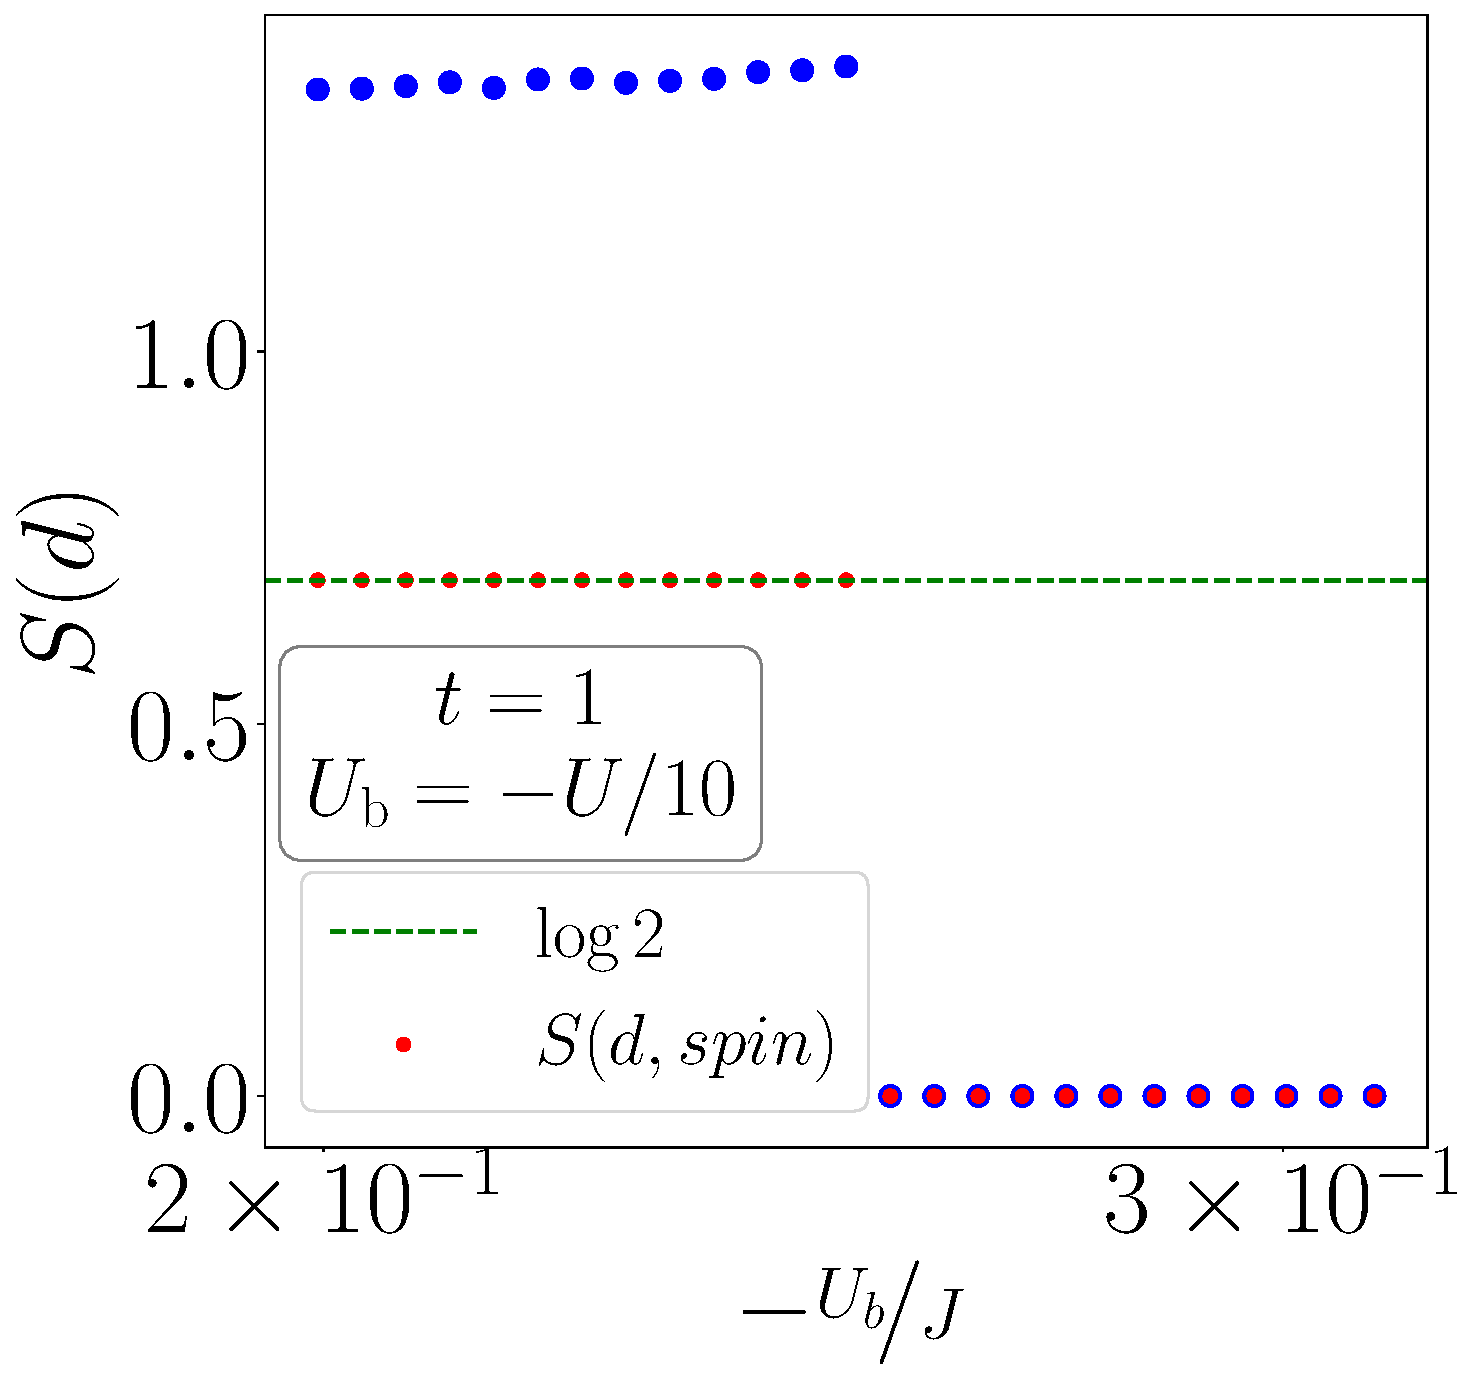
\includegraphics[width=0.32\textwidth]{../figures/EE-d-D=1000.00000,t=1.00000,J=30.00000,V=1.50000J,Ub=-Uby10,N=4,U=59.85787,93.55363,25.pdf}
	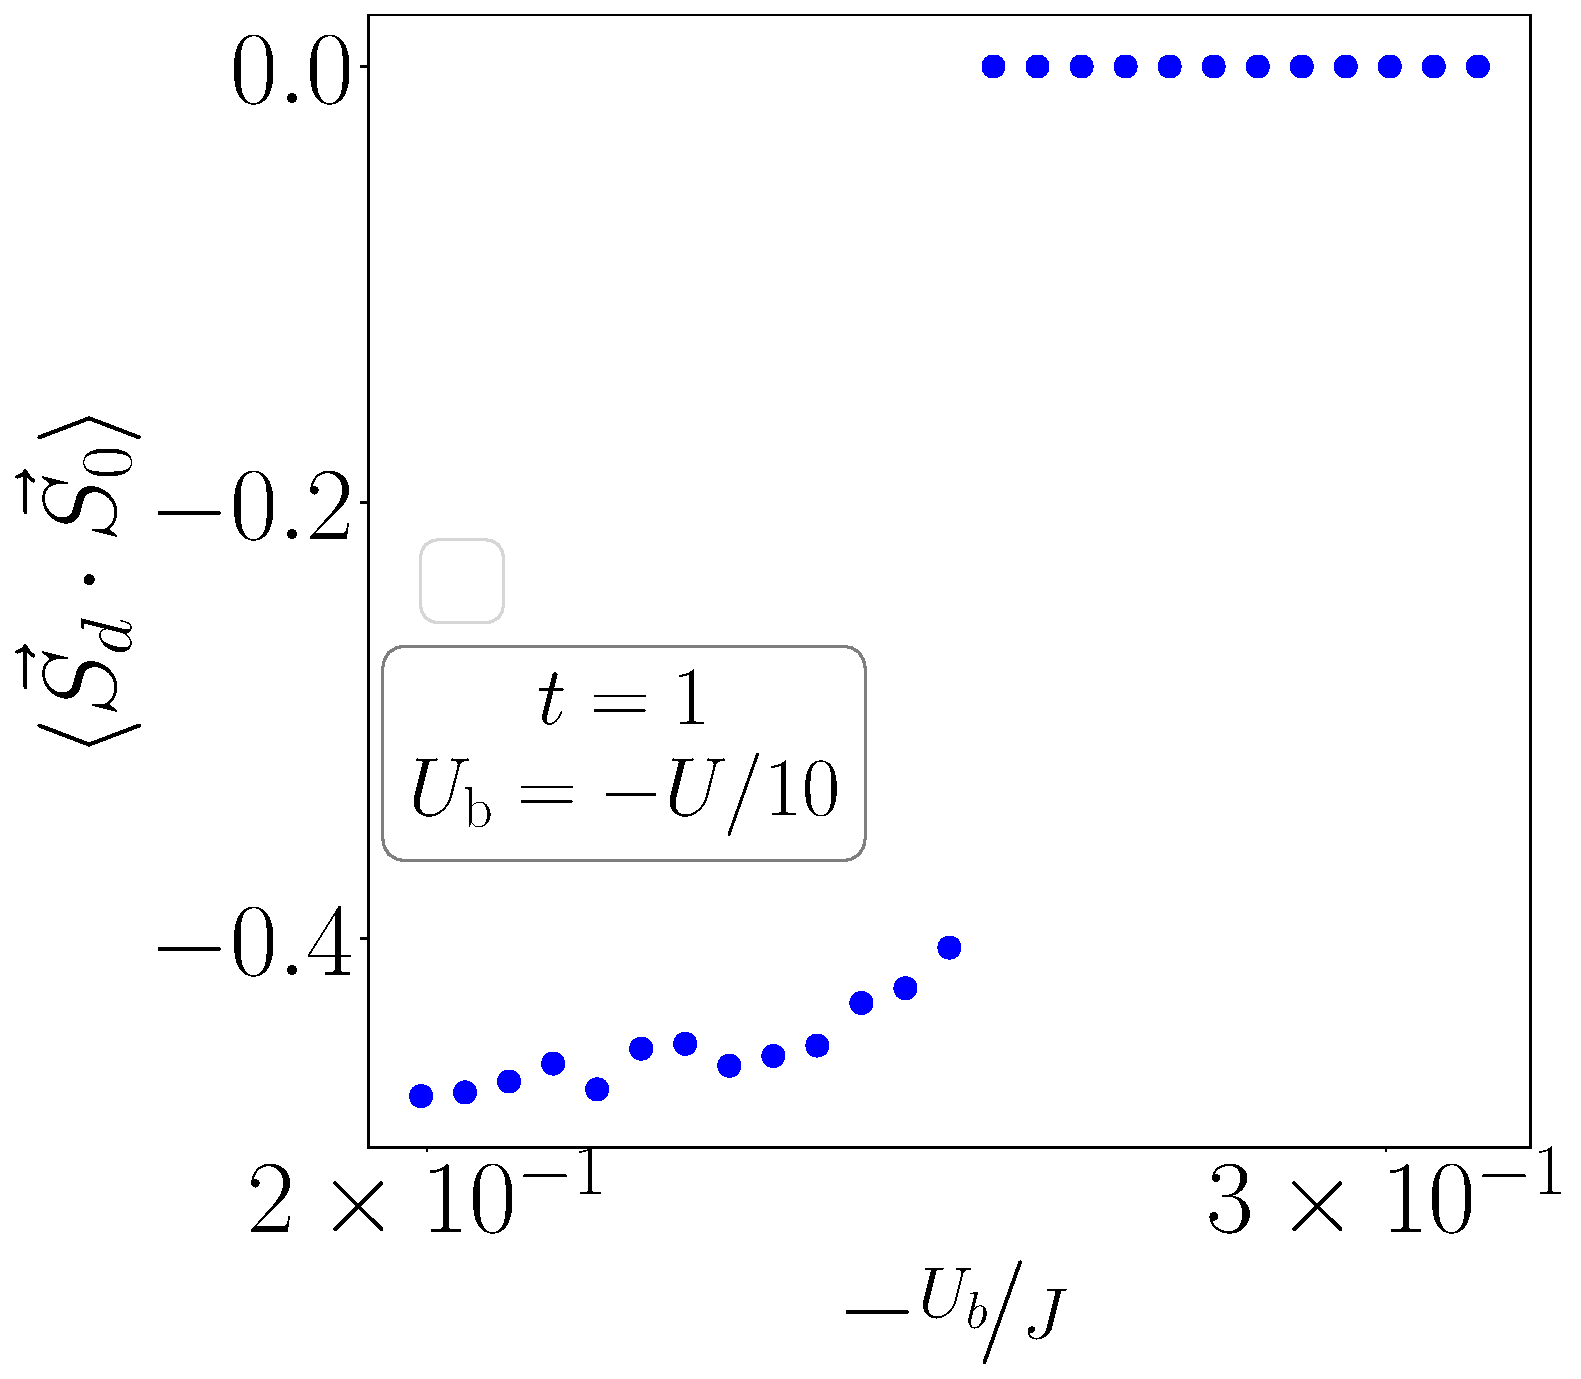
\includegraphics[width=0.32\textwidth]{../figures/corr-d0-D=1000.00000,t=1.00000,J=30.00000,V=1.50000J,Ub=-Uby10,N=4,U=59.85787,93.55363,25.pdf}
	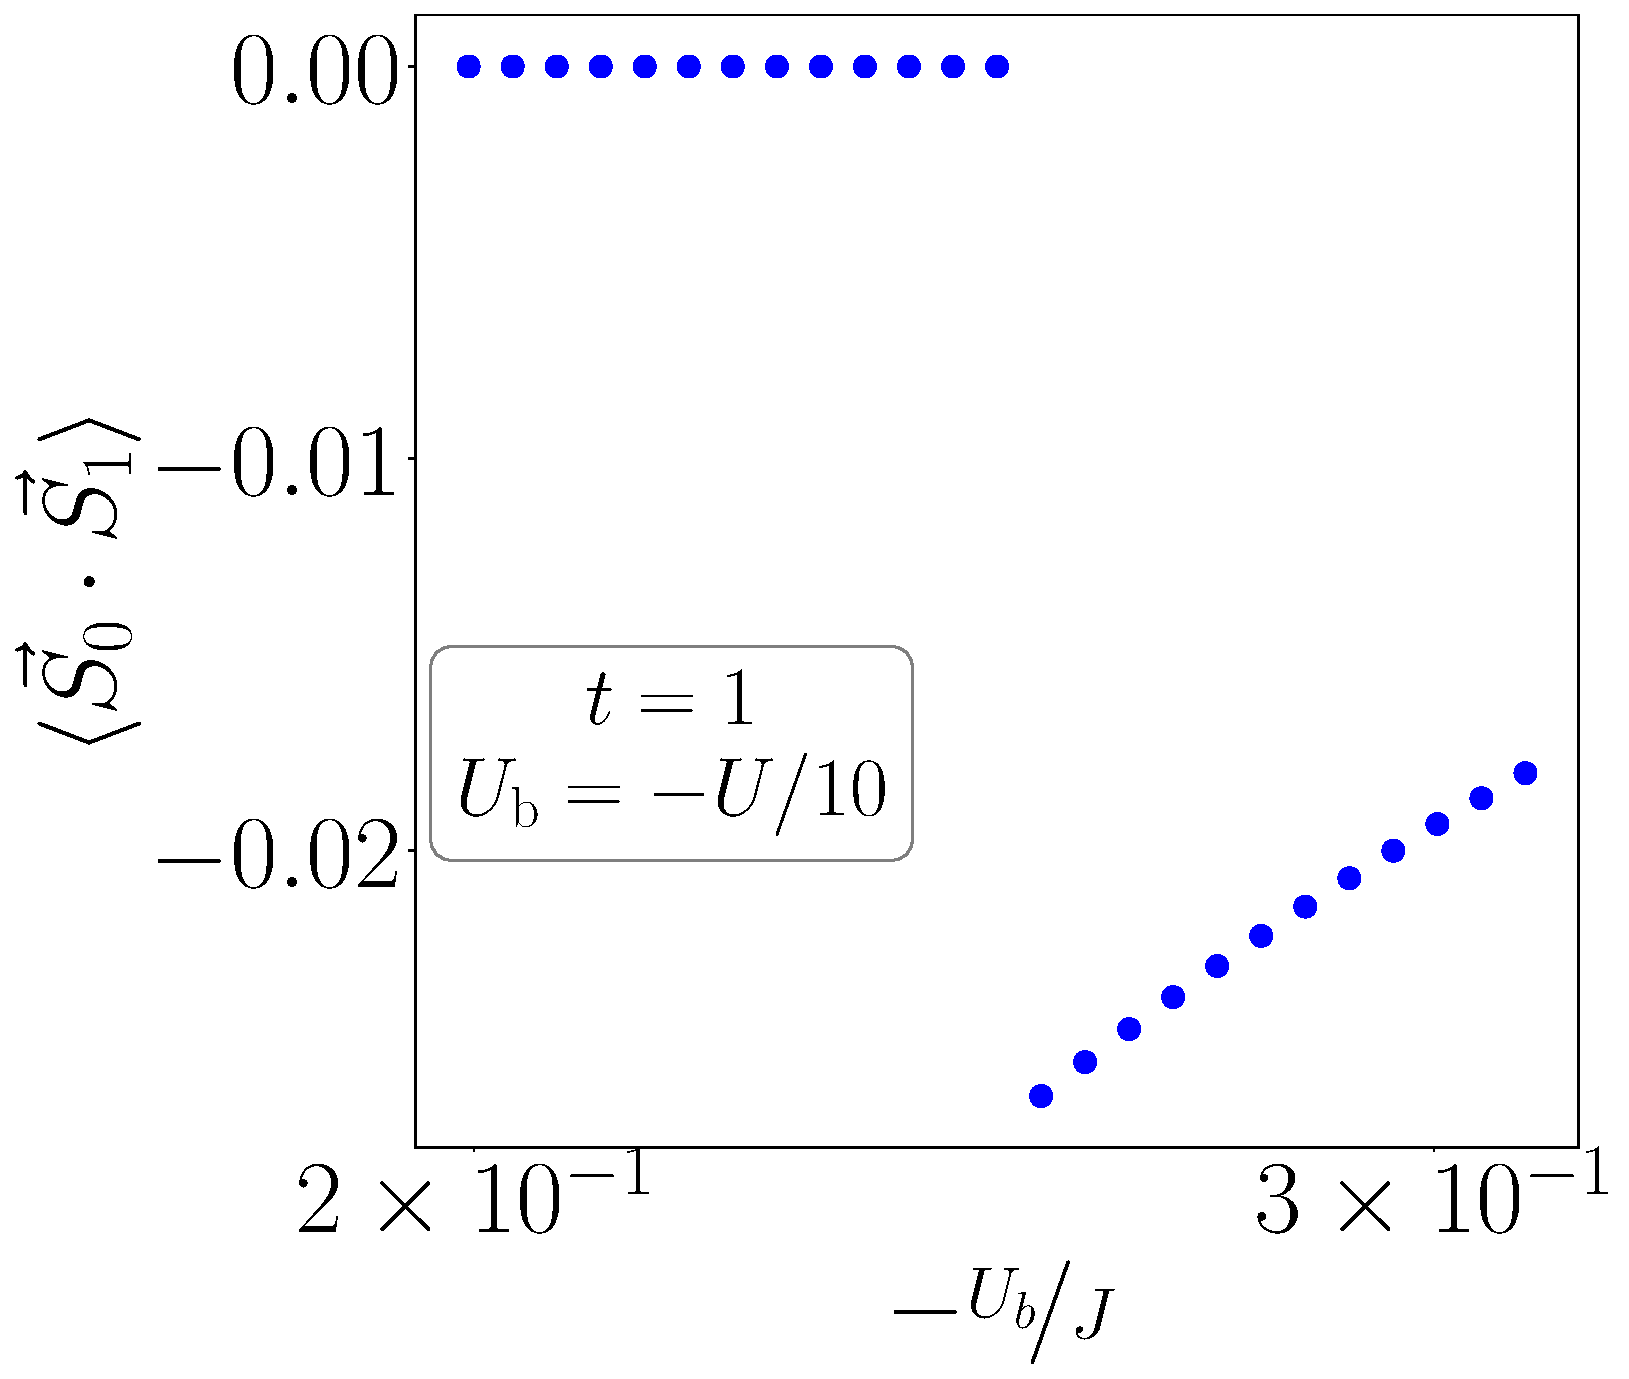
\includegraphics[width=0.32\textwidth]{../figures/r-vec-corr-01-D=1000.00000,t=1.00000,J=30.00000,V=1.50000J,Ub=-Uby10,N=4,U=59.85787,93.55363,25.pdf}
\end{center}

\subsection*{Real-space correlations}
\begin{center}
	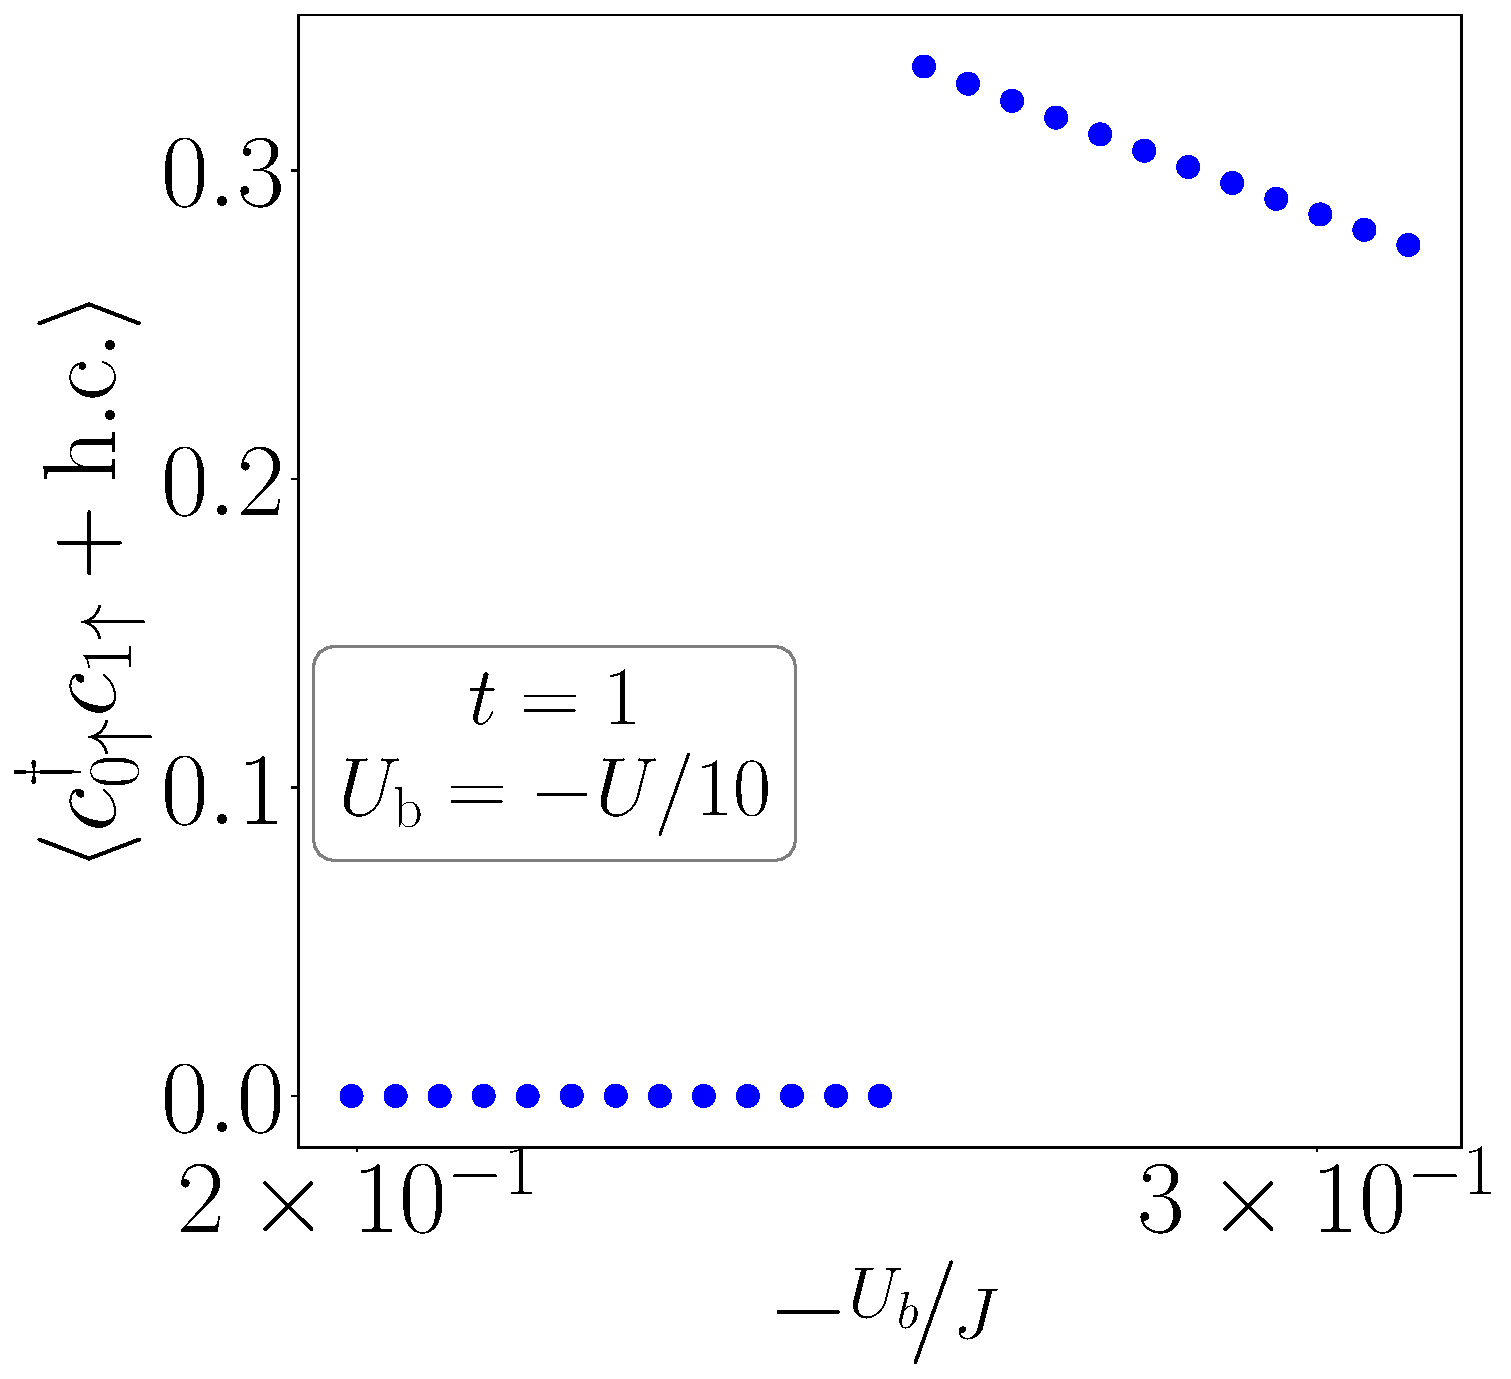
\includegraphics[width=0.32\textwidth]{../figures/r1p-D=1000.00000,t=1.00000,J=30.00000,V=1.50000J,Ub=-Uby10,N=4,U=59.85787,93.55363,25.pdf}
	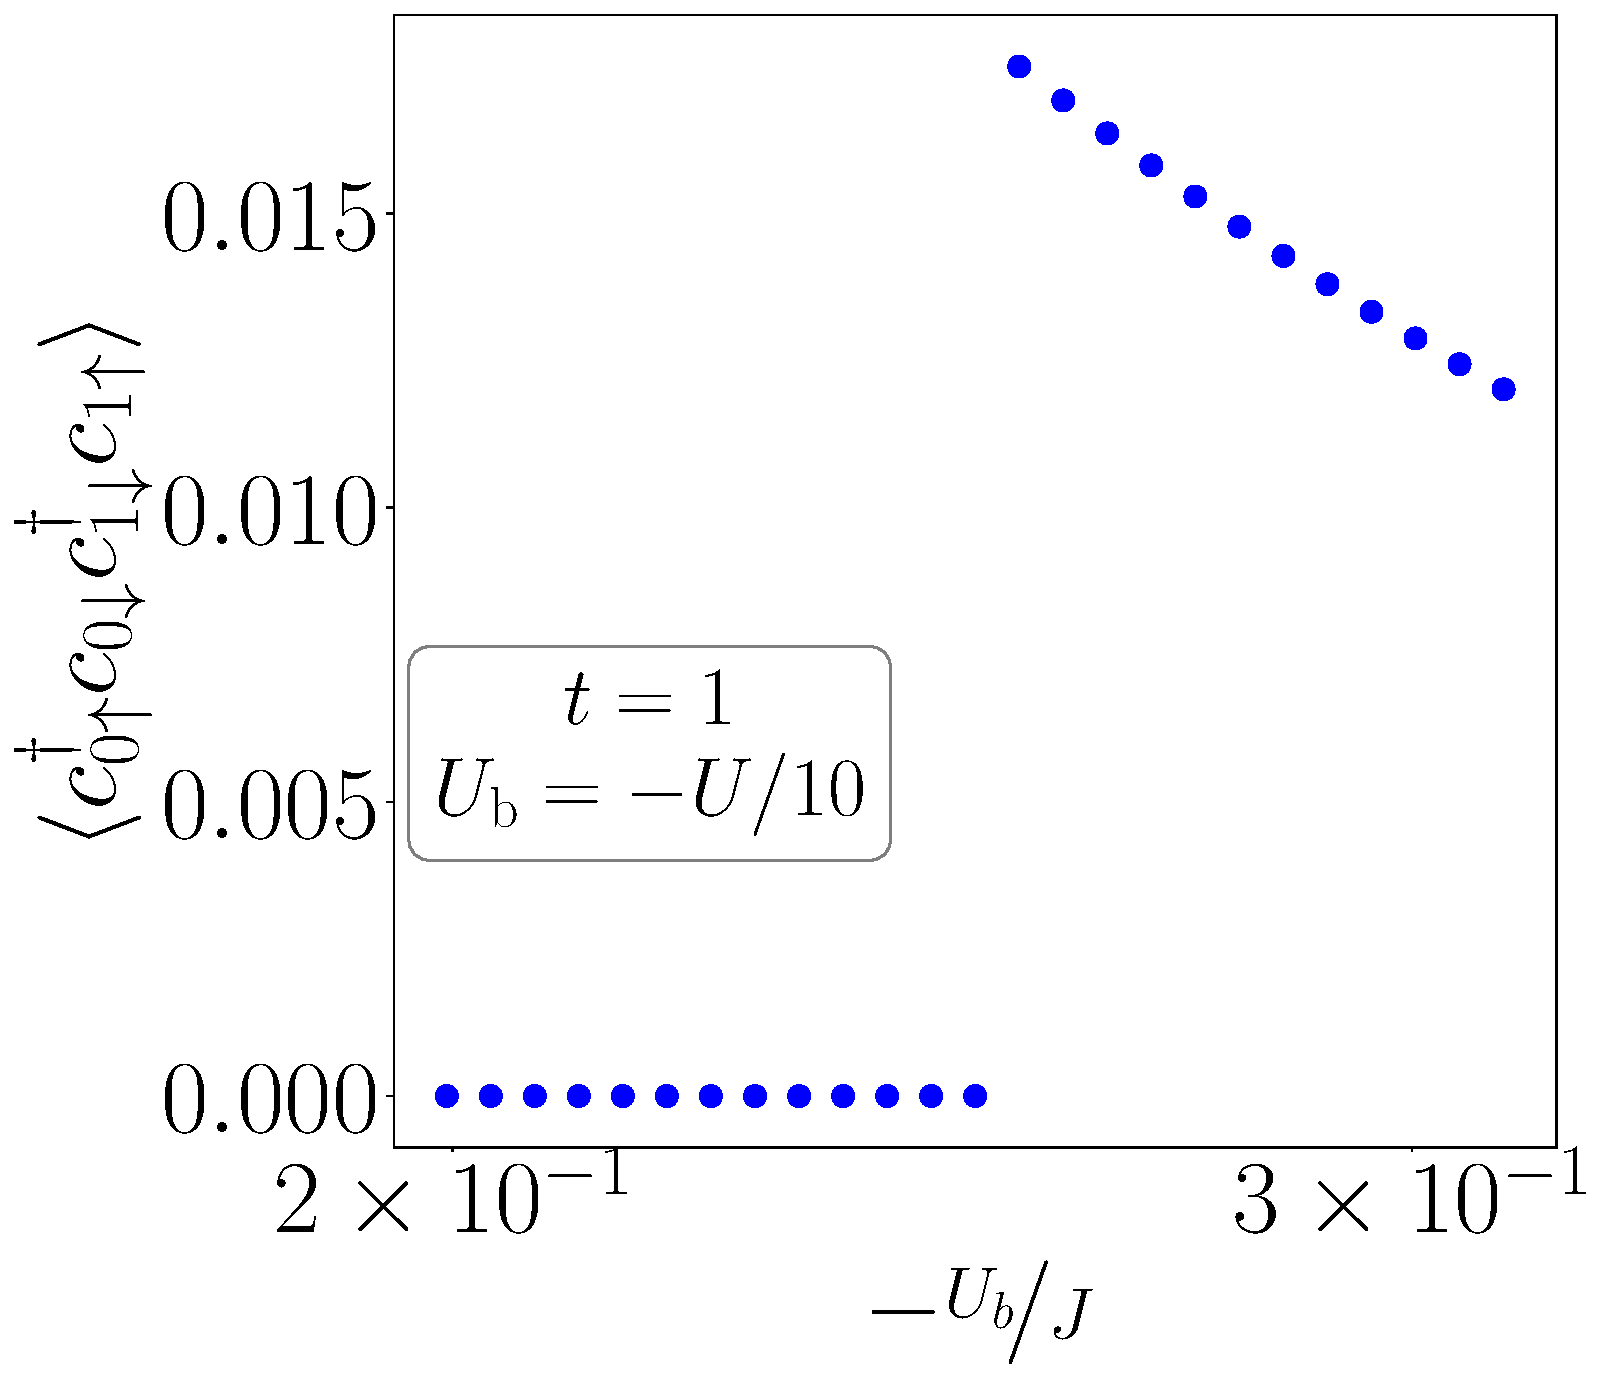
\includegraphics[width=0.32\textwidth]{../figures/r-od-D=1000.00000,t=1.00000,J=30.00000,V=1.50000J,Ub=-Uby10,N=4,U=59.85787,93.55363,25.pdf}
	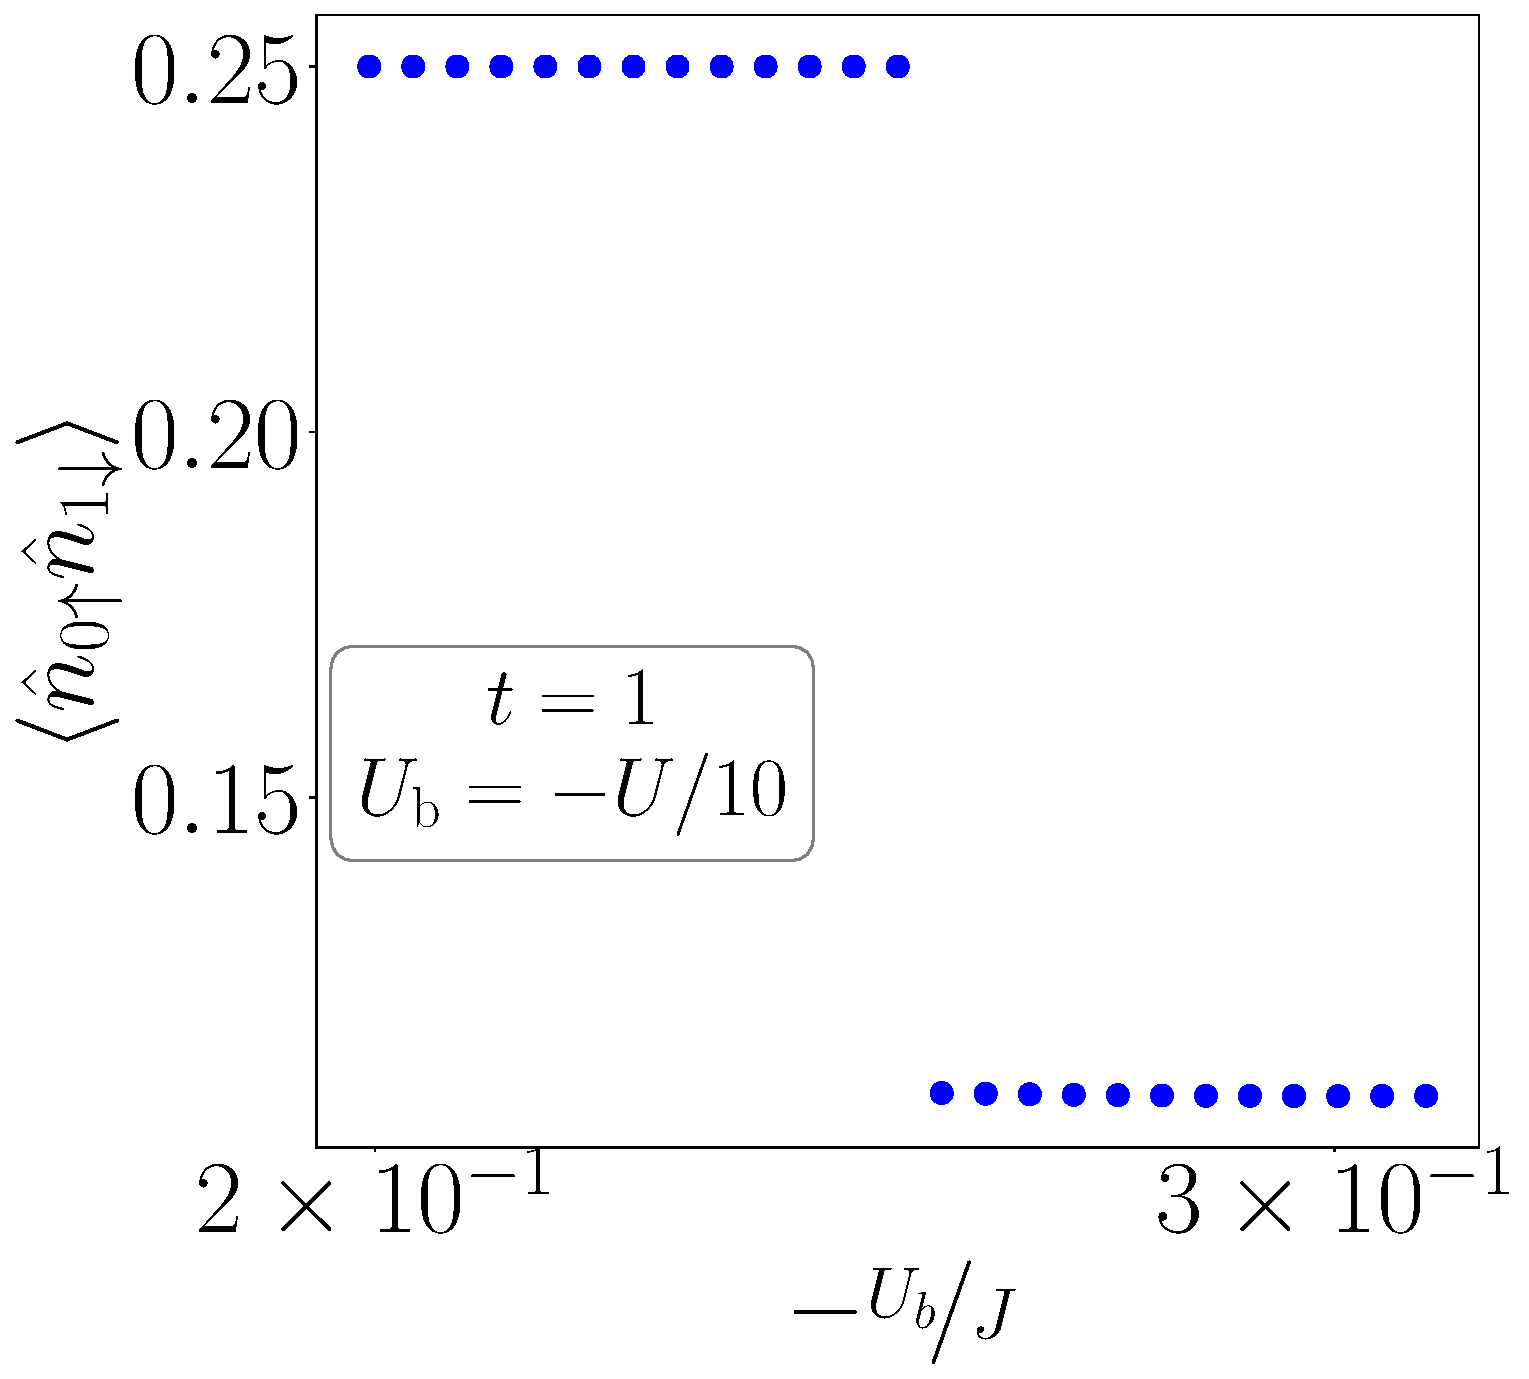
\includegraphics[width=0.32\textwidth]{../figures/r-opp-D=1000.00000,t=1.00000,J=30.00000,V=1.50000J,Ub=-Uby10,N=4,U=59.85787,93.55363,25.pdf}

	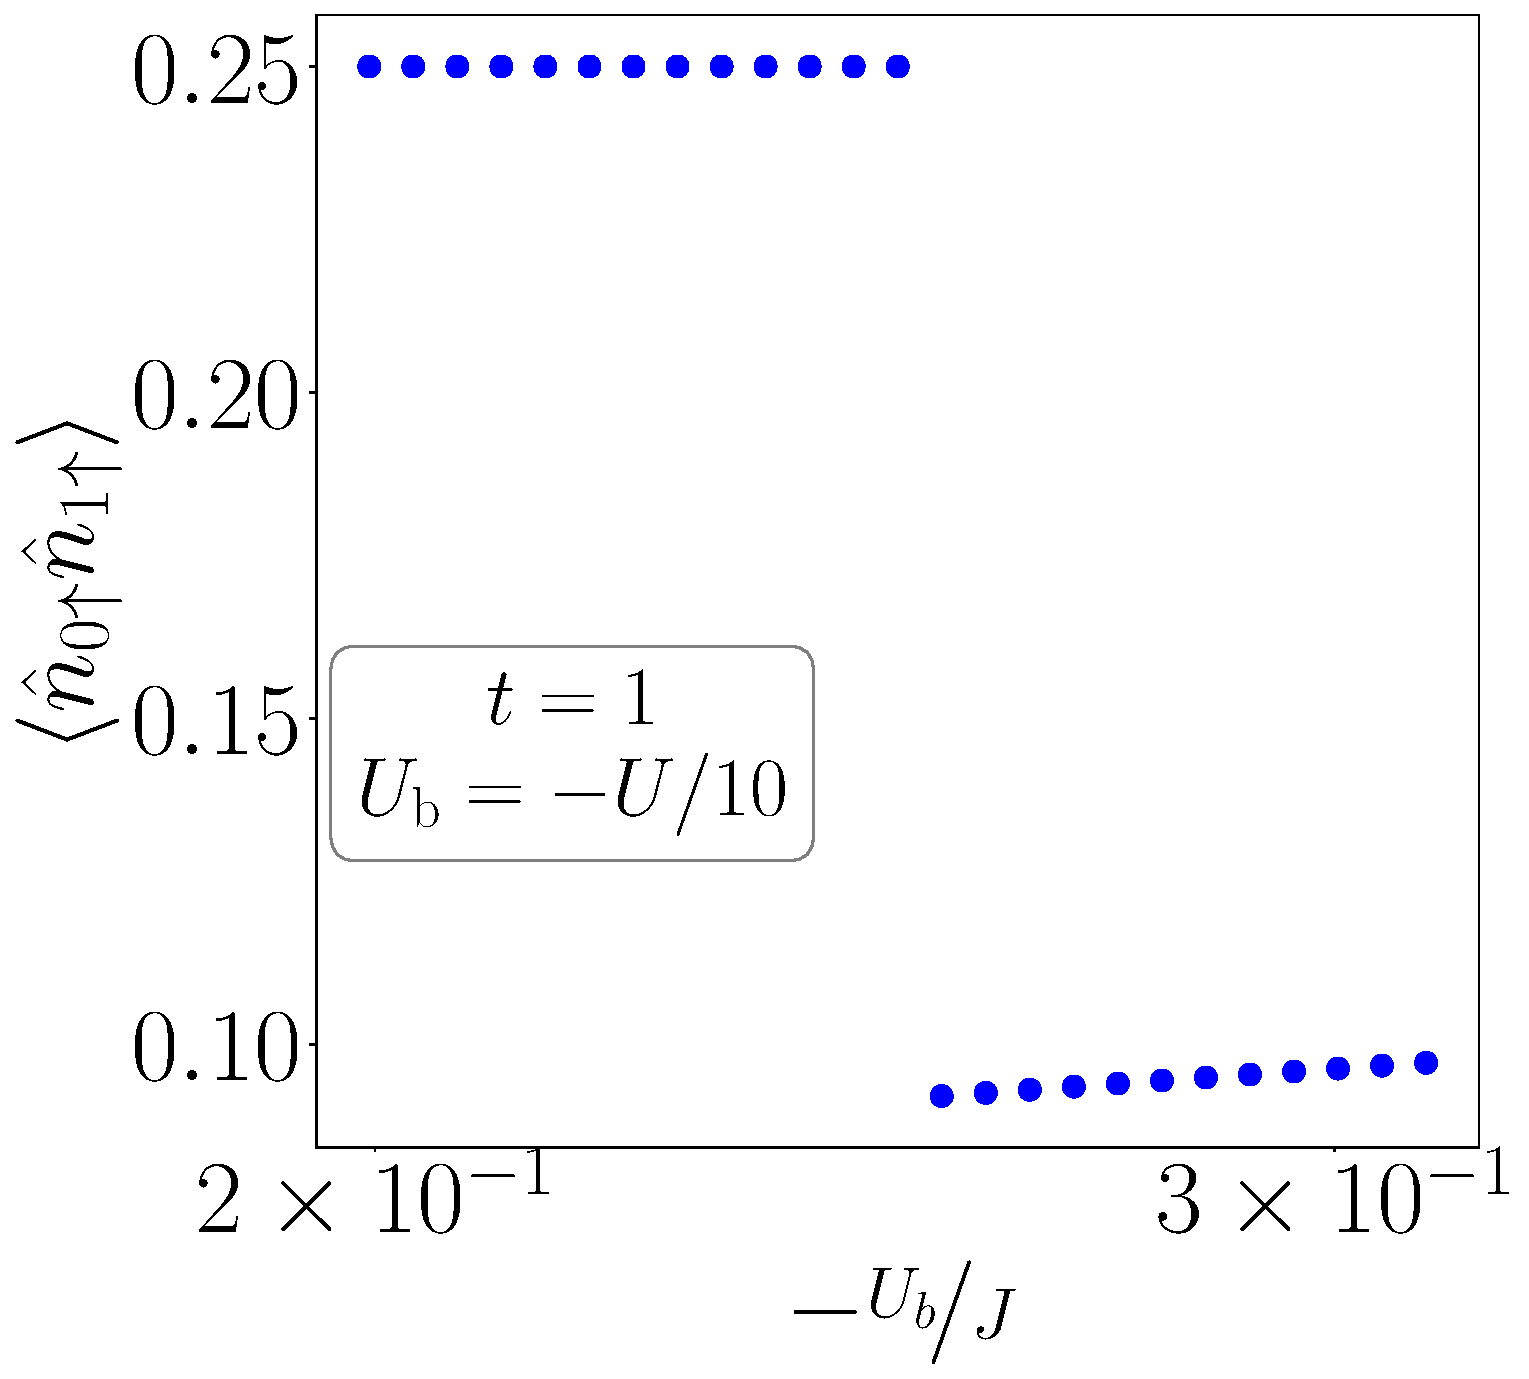
\includegraphics[width=0.3\textwidth]{../figures/r-par-D=1000.00000,t=1.00000,J=30.00000,V=1.50000J,Ub=-Uby10,N=4,U=59.85787,93.55363,25.pdf}
	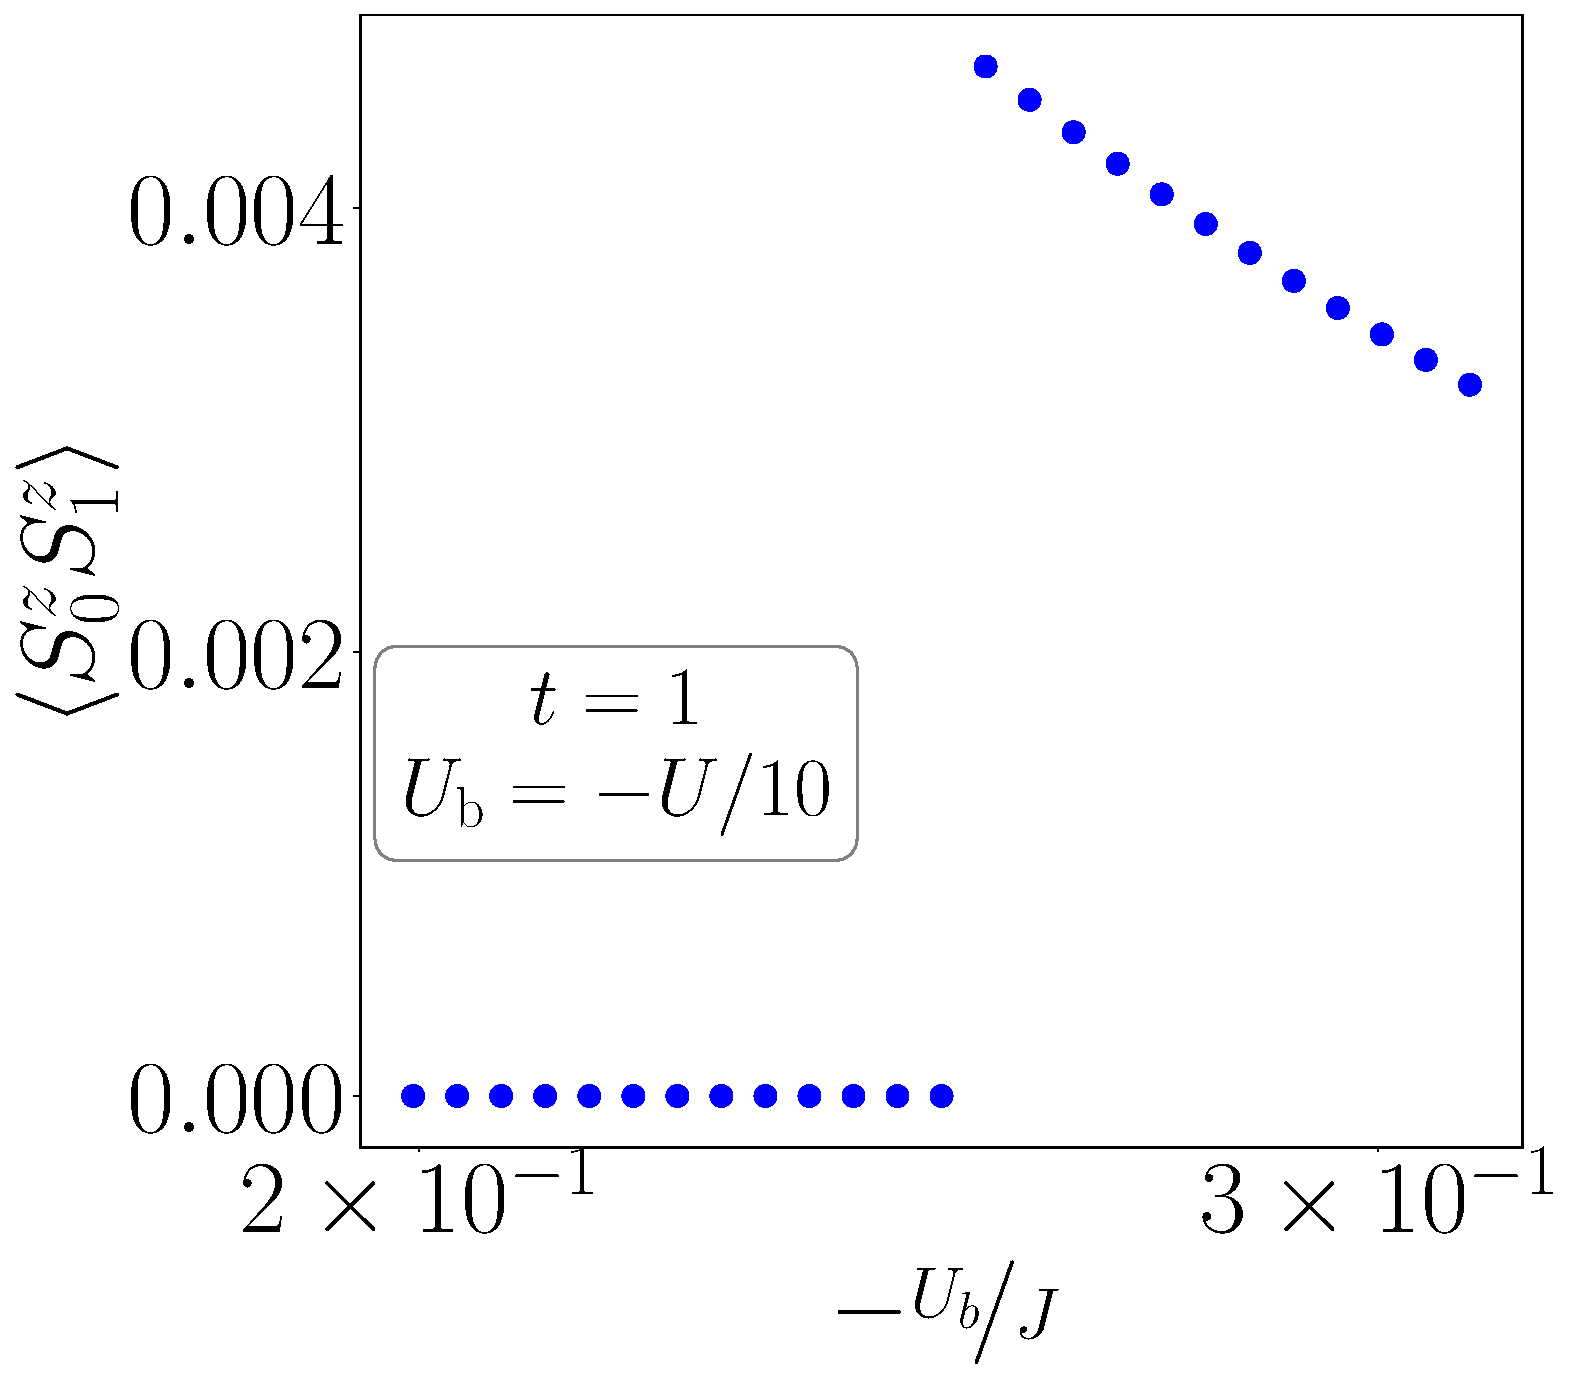
\includegraphics[width=0.3\textwidth]{../figures/r-ising-D=1000.00000,t=1.00000,J=30.00000,V=1.50000J,Ub=-Uby10,N=4,U=59.85787,93.55363,25.pdf}
	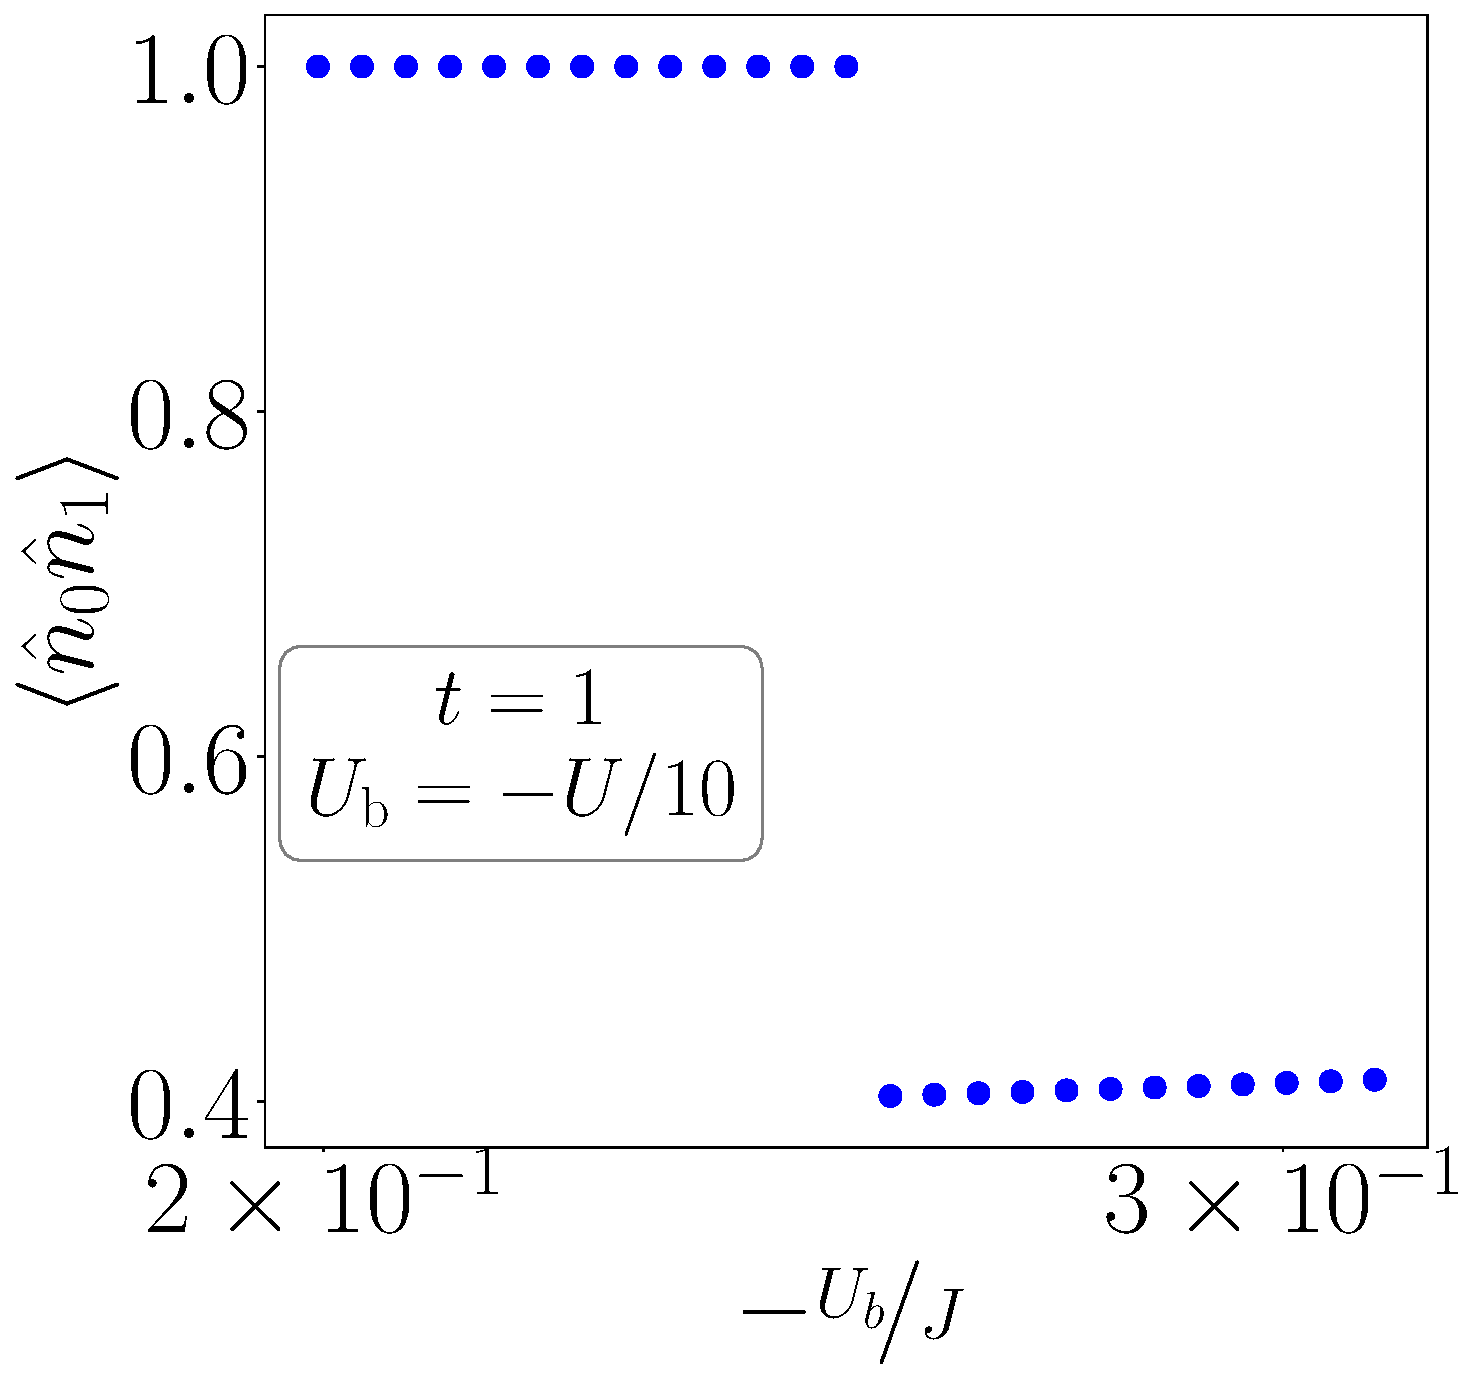
\includegraphics[width=0.3\textwidth]{../figures/r-charge-D=1000.00000,t=1.00000,J=30.00000,V=1.50000J,Ub=-Uby10,N=4,U=59.85787,93.55363,25.pdf}
\end{center}

\section{Presence of sub-dominant pair fluctuations}
\begin{center}
	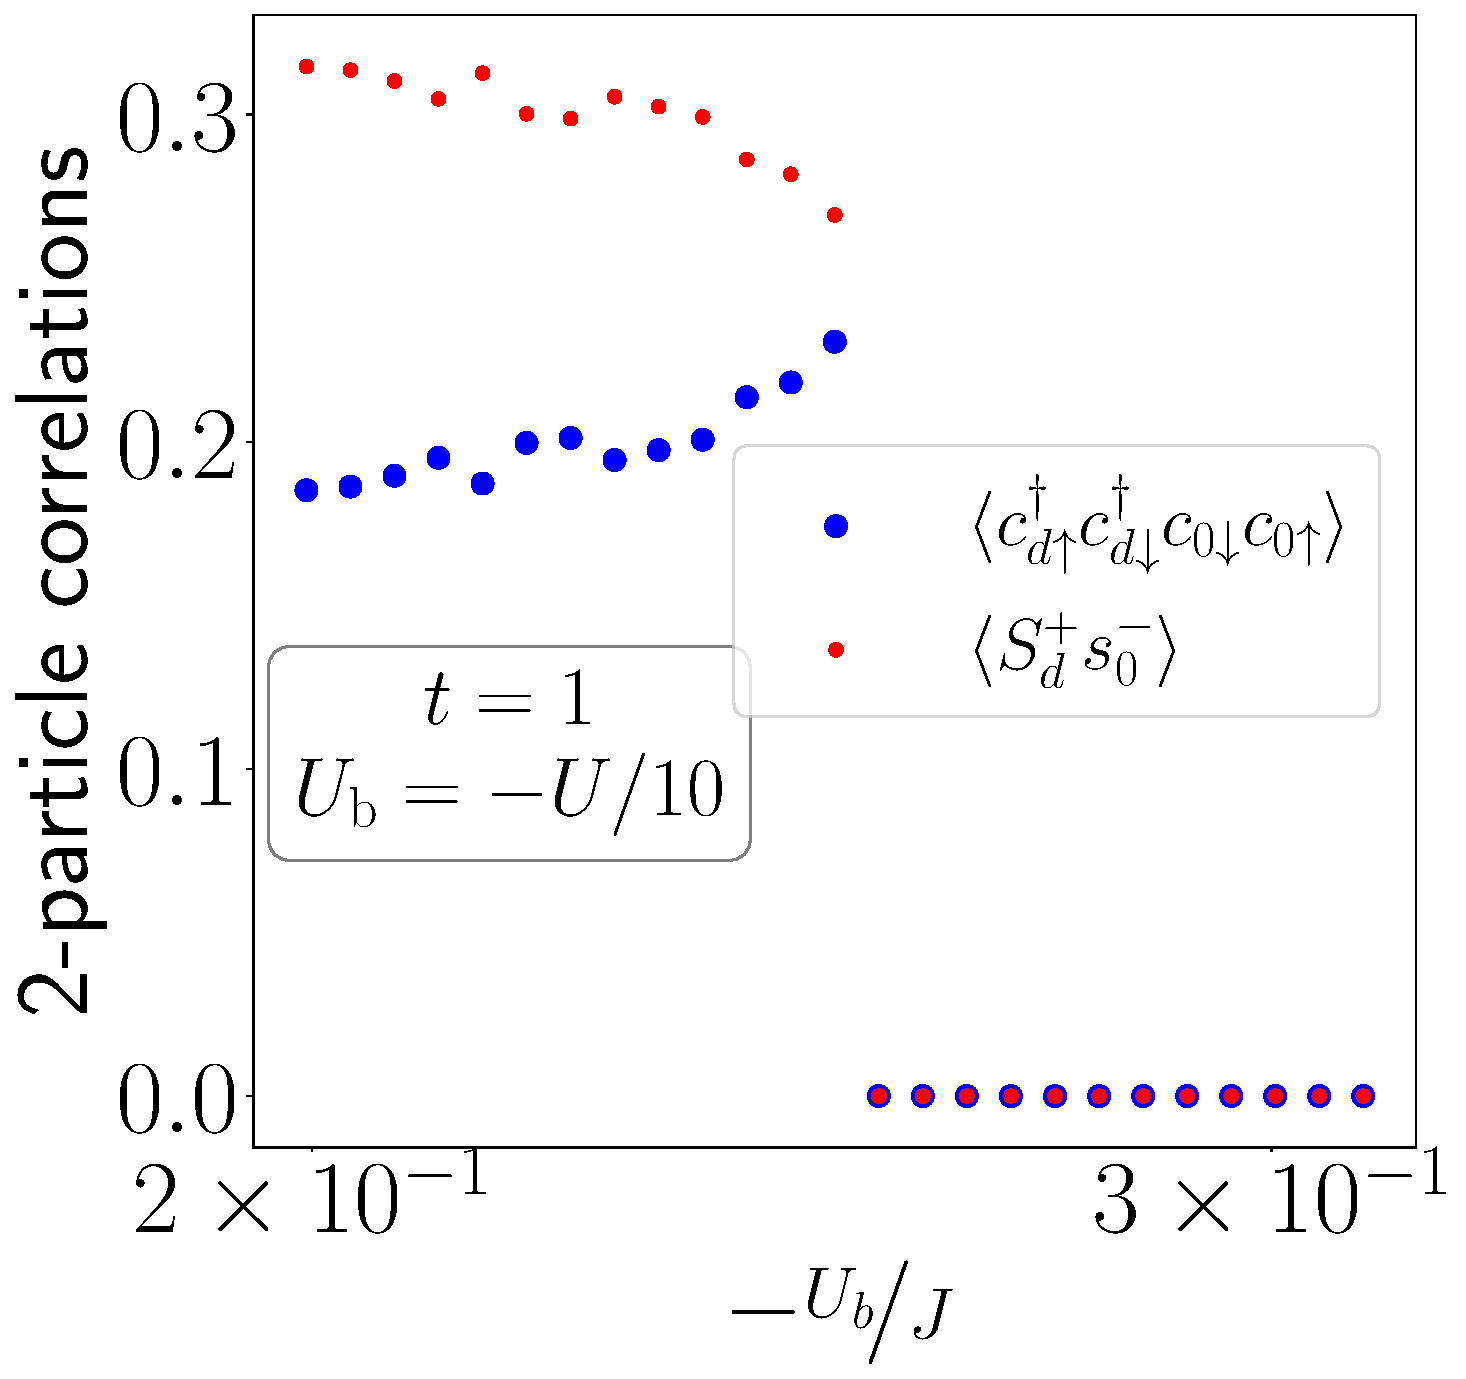
\includegraphics[width=0.4\textwidth]{../figures/odlro-D=1000.00000,t=1.00000,J=30.00000,V=1.50000J,Ub=-Uby10,N=4,U=59.85787,93.55363,25.pdf}
	\captionof{figure}{Growth of pair fluctuations \(p^\dagger_d p_0\) between the impurity and the zeroth site towards the critical point, \(p^\dagger=c^\dagger_\uparrow c^\dagger_\downarrow\) being the local pair creation operator. This comes at the cost of the spin-flip fluctuations \(S_d^+ s_0^- + \text{h.c.}\). which decrease towards the transition.}
	\label{pair_fluc}
\end{center}

The behaviour of the various kinds of correlation functions (for eg., the reduction of the impurity compensation \(\vec{S}_d\cdot\vec{s}_0\)) shown above indicate that the Kondo cloud that screens the impurity is getting destroyed as \(U_b/J\) increases in magnitude. To shed some light on the nature of the fluctuations that faciliate this process, we also plot the average pair fluctuation in the ground state as a function of \(U_b/J\), in fig.~\ref{pair_fluc}. The pair fluctuations are terms that transfer an electron pair between the impurity and zeroth sites: \(c^\dagger_{d \uparrow}c^\dagger_{d \downarrow} c_{0 \downarrow}c_{0 \uparrow}\). It can be seen from the figure that while the spin-flip fluctuations decrease (since the Kondo cloud is formed out of these spin-flip fluctuations, this is consistent with the destruction of the Kondo cloud discussed in this paragraph), the pair fluctuations pick up. Since the spin subspace and charge subspace cannot coincide on the same site, we can then conclude that it is the growth of these pair fluctuations brought about by the presence of the purely local interaction \(U_b\) that make the screening of the impurity spin very poor.

\section{Spectral functions}

\subsection{Impurity spectral function \(A_{dd}(\omega)\)}
These are the frequency-domain spectral functions for the retarded propagator \(-i\theta(t)\left<\left\{c_{d\sigma}(t),c^\dagger_{d\sigma}\right\}  \right>\):
\begin{center}
	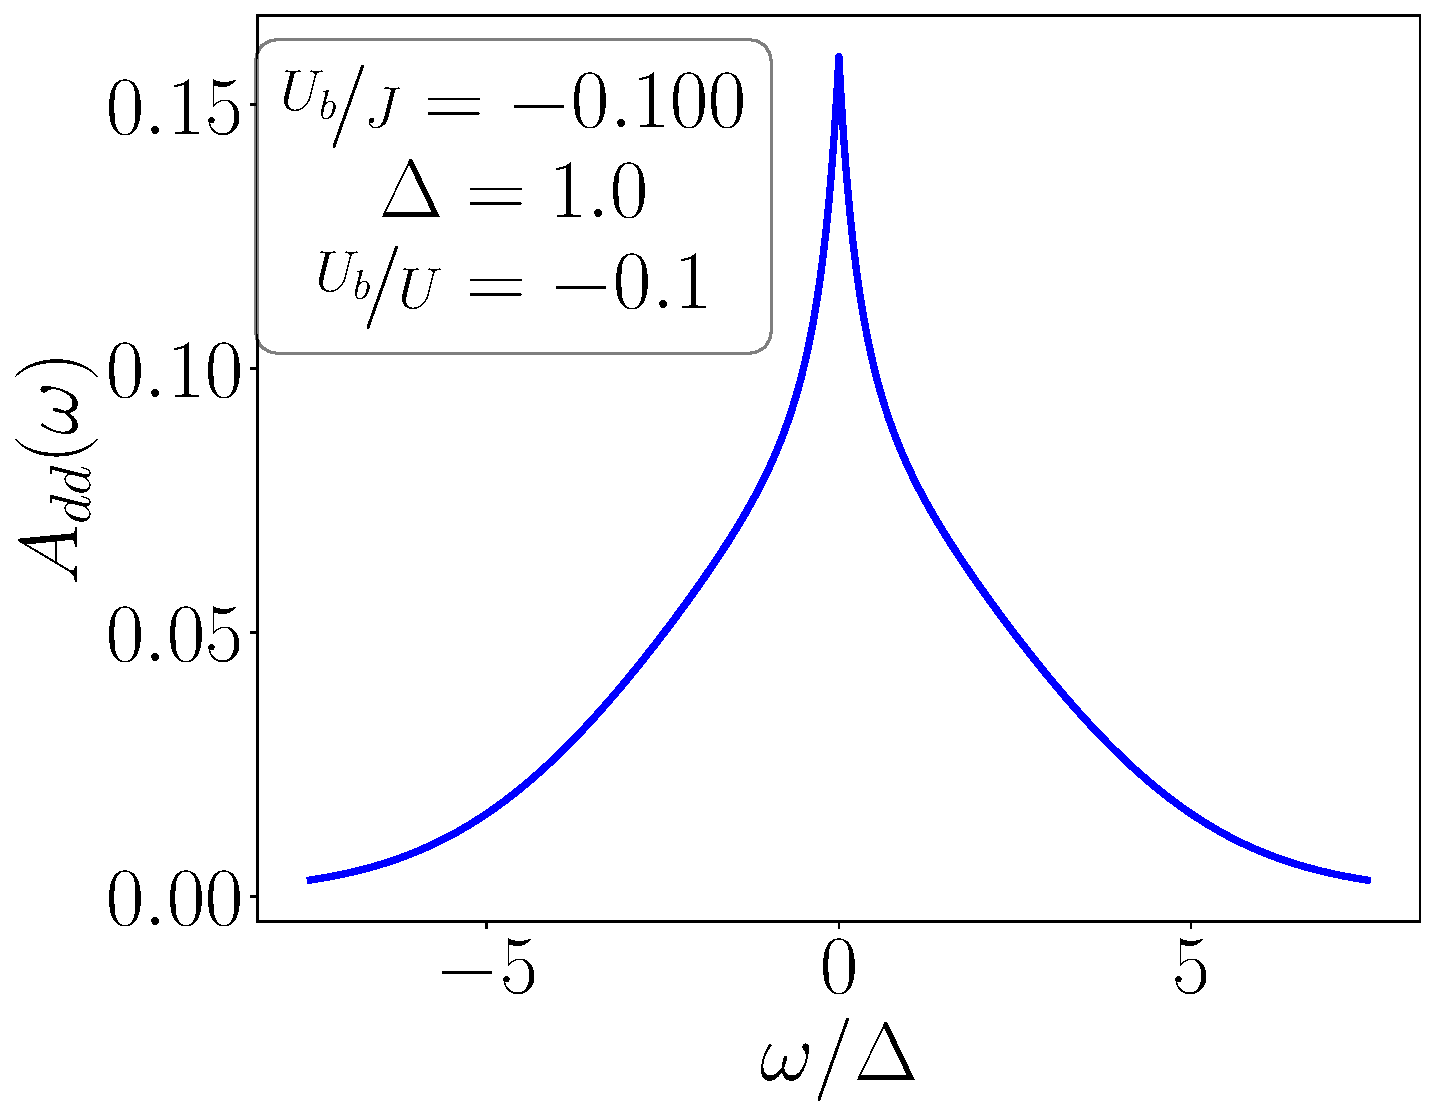
\includegraphics[width=0.45\textwidth]{../figures/spec_func_Ub_by_J=-0.100.pdf}
	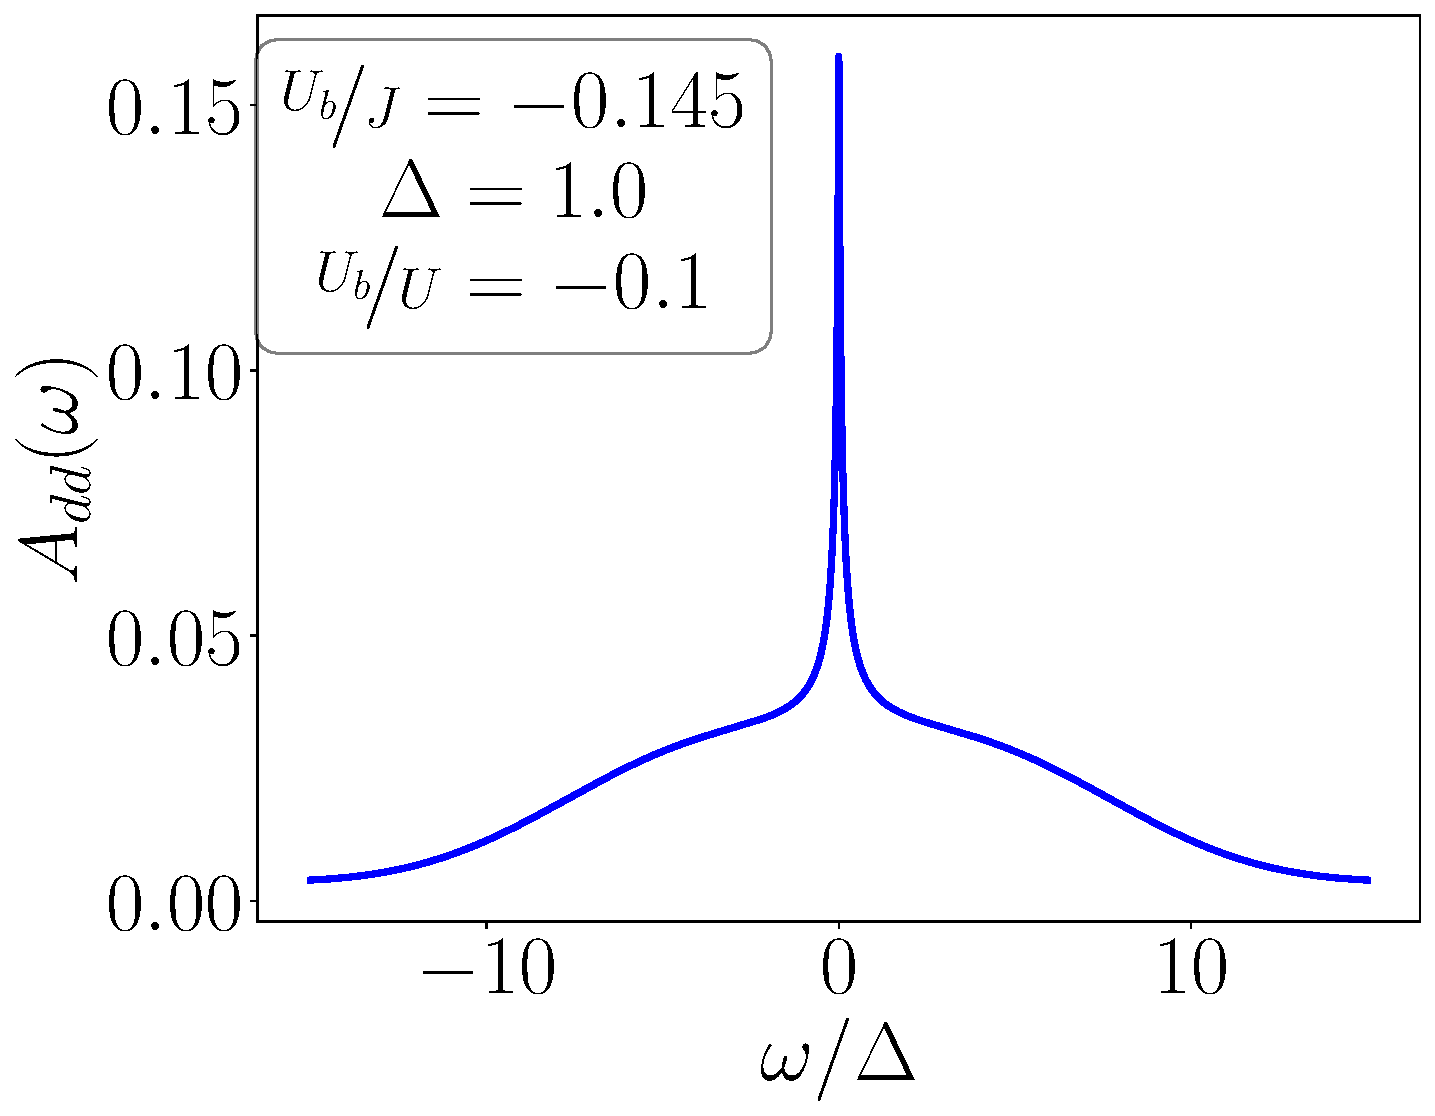
\includegraphics[width=0.45\textwidth]{../figures/spec_func_Ub_by_J=-0.145.pdf}
	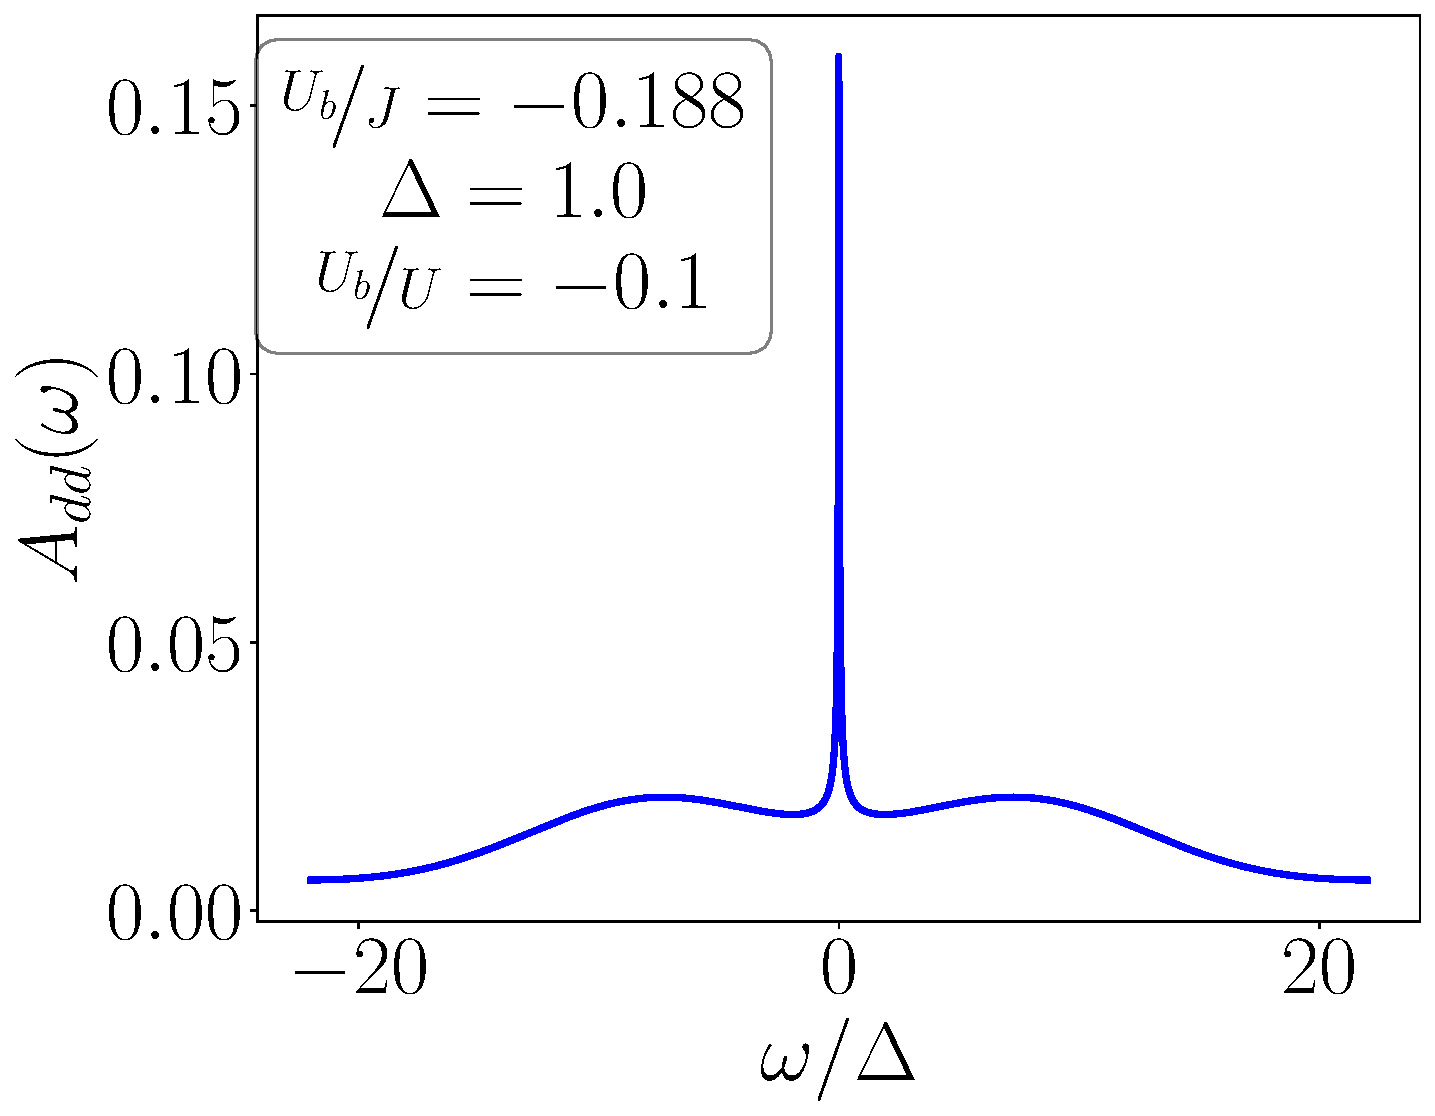
\includegraphics[width=0.45\textwidth]{../figures/spec_func_Ub_by_J=-0.188.pdf}
	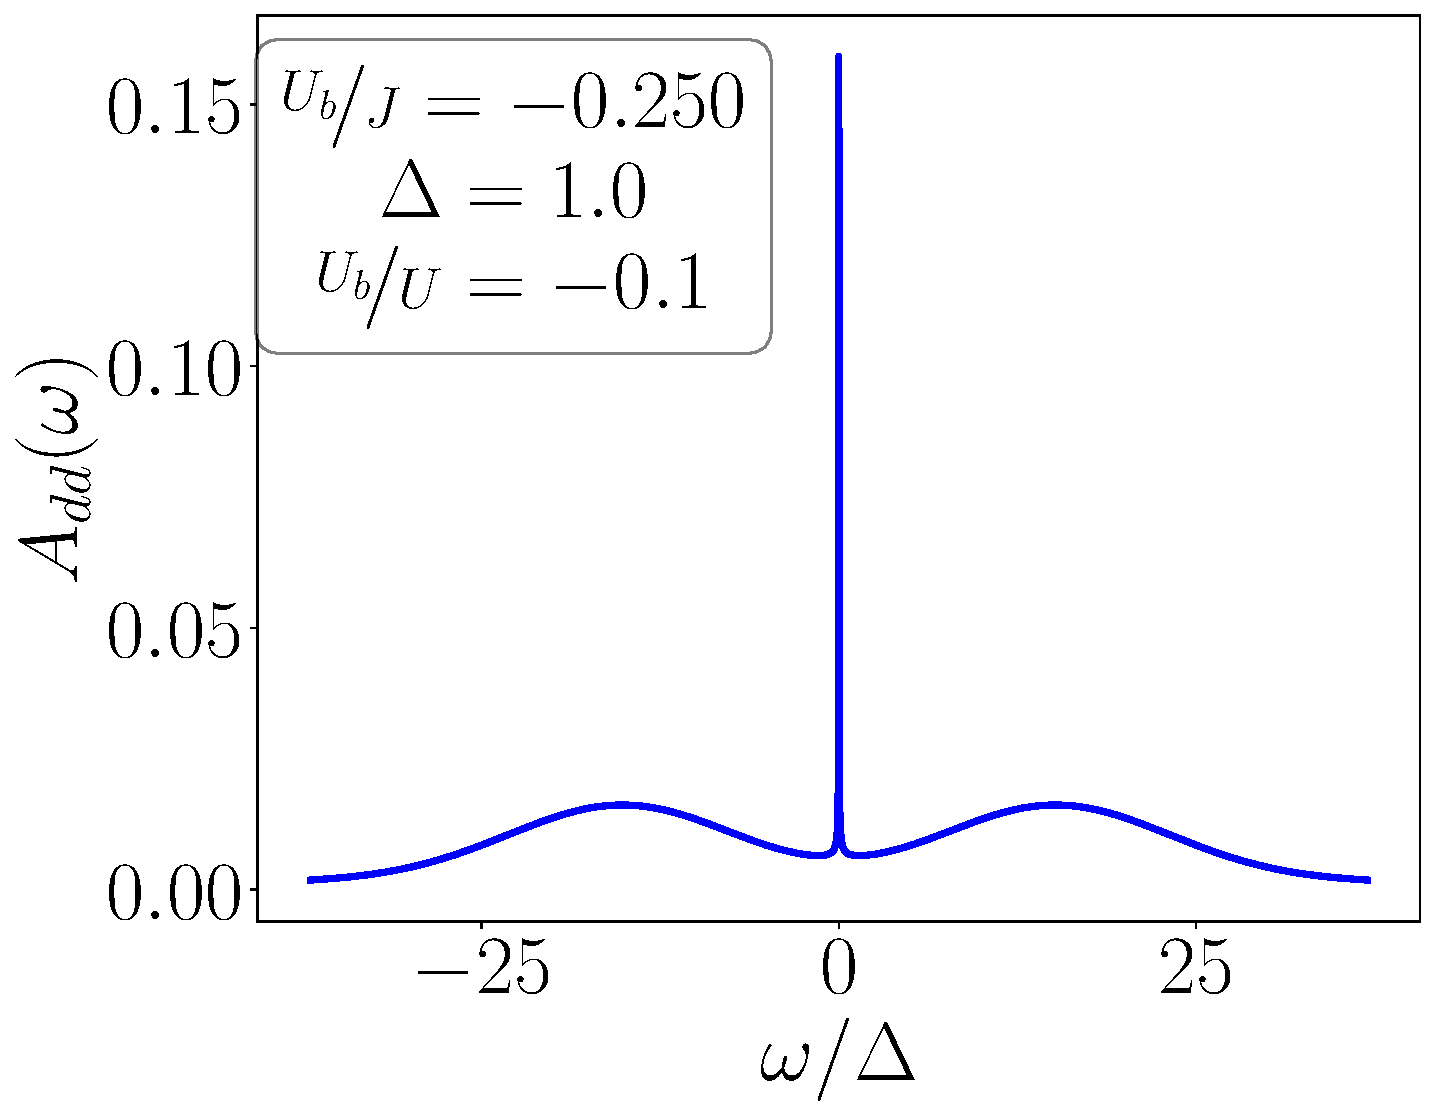
\includegraphics[width=0.45\textwidth]{../figures/spec_func_Ub_by_J=-0.250.pdf}
	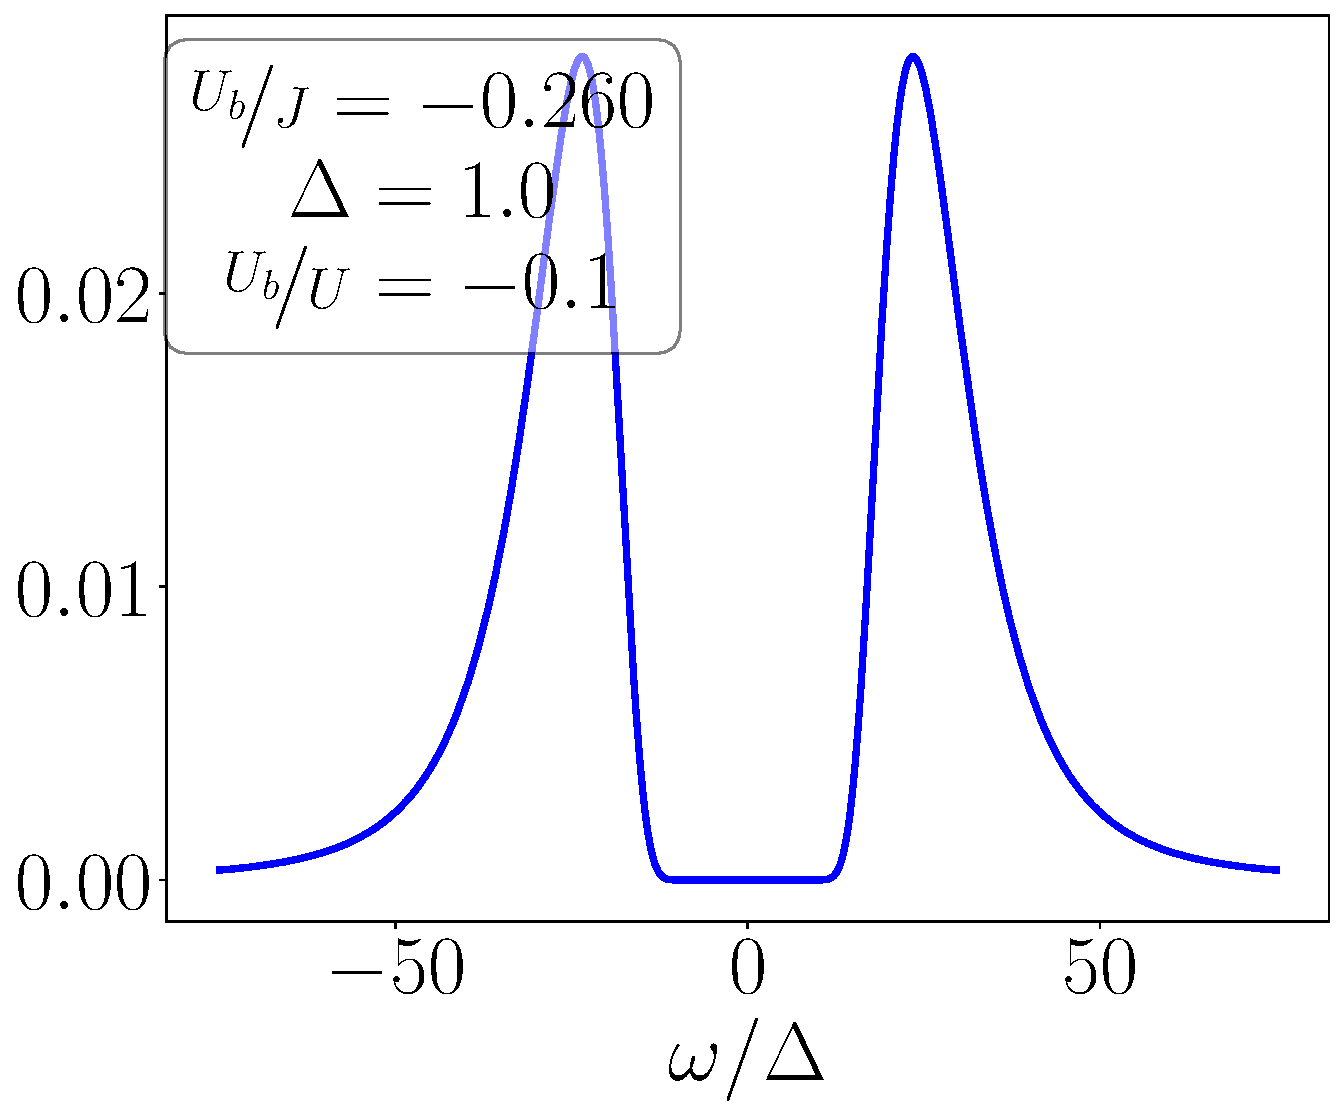
\includegraphics[width=0.45\textwidth]{../figures/spec_func_Ub_by_J=-0.26.pdf}
	\label{spec_func_fig}
\end{center}

\subsection{Impurity-bath off-diagonal spectral function \(A_{dz}(\omega)\)}
These are the frequency-domain spectral functions for the off-diagonal retarded propagator \(-i\theta(t)\left<\left\{c_{d\sigma}(t),c^\dagger_{0\sigma}\right\}  \right>\):
\begin{center}
	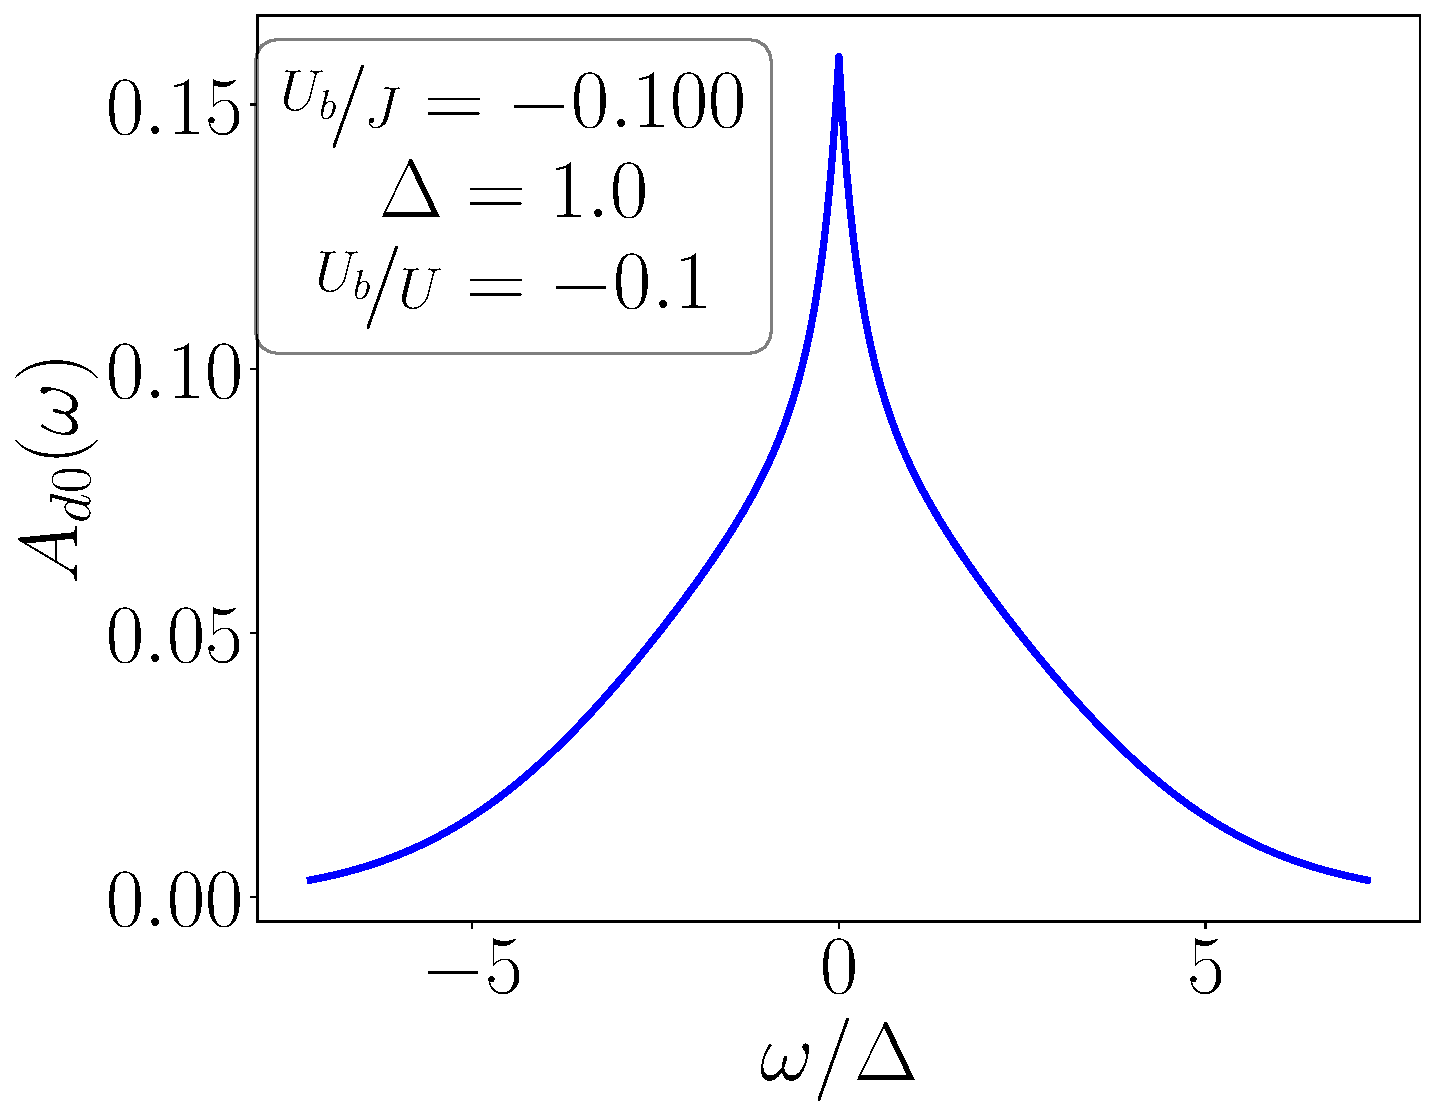
\includegraphics[width=0.45\textwidth]{../figures/spec_func_d0_Ub_by_J=-0.100.pdf}
	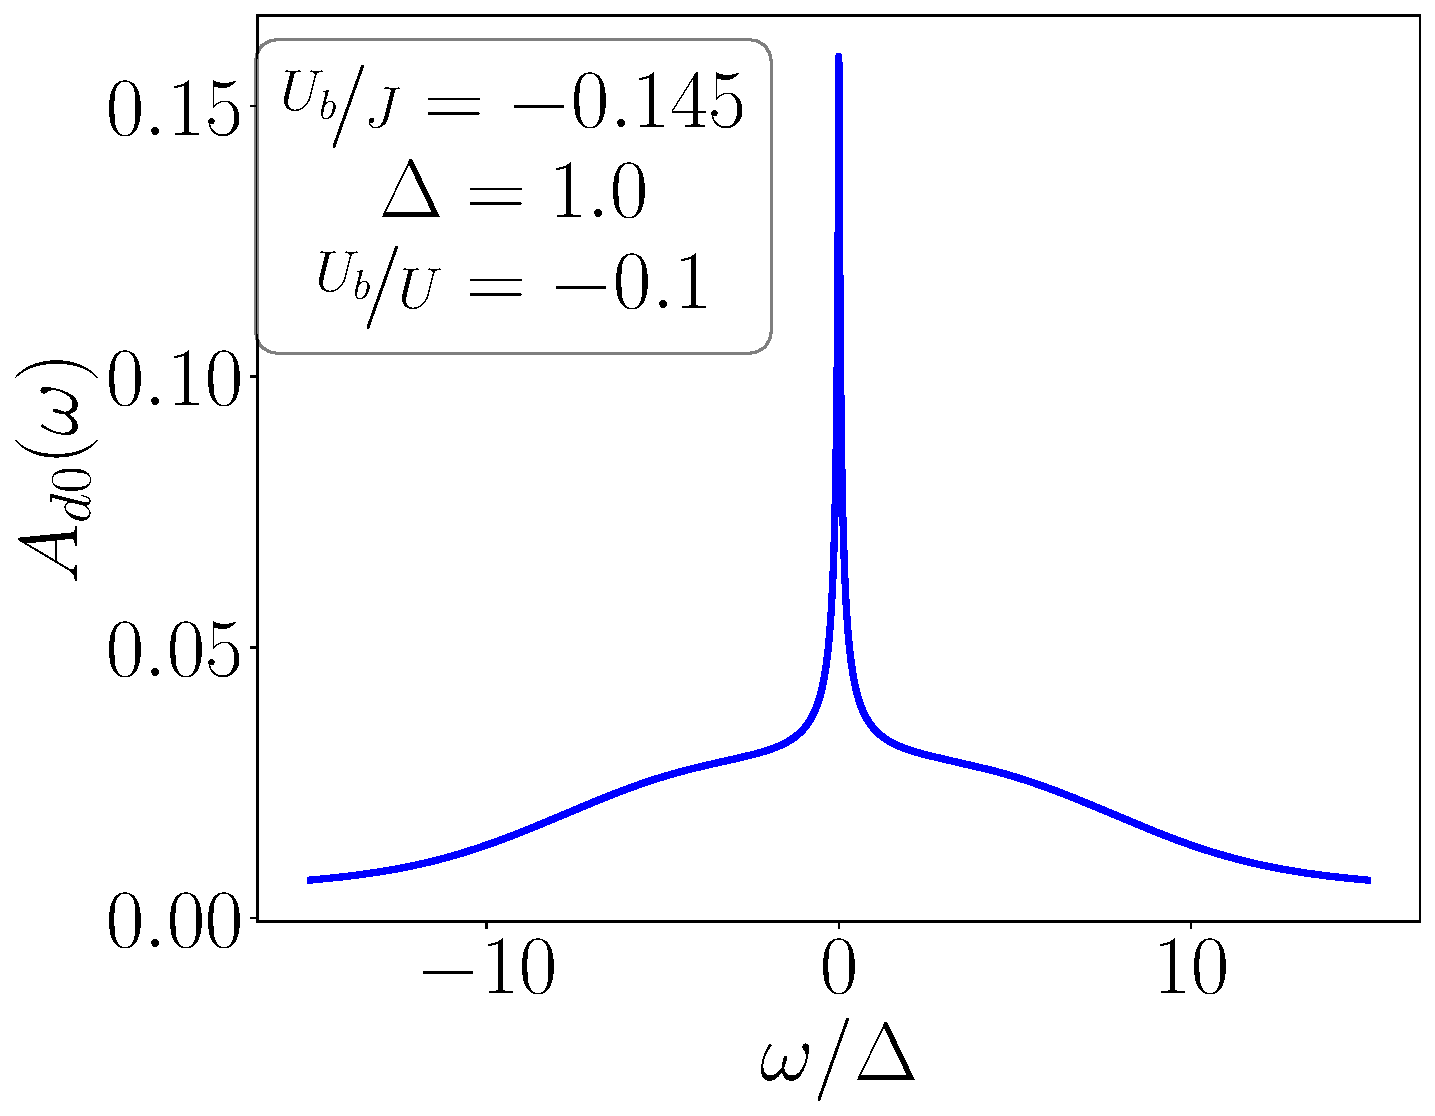
\includegraphics[width=0.45\textwidth]{../figures/spec_func_d0_Ub_by_J=-0.145.pdf}
	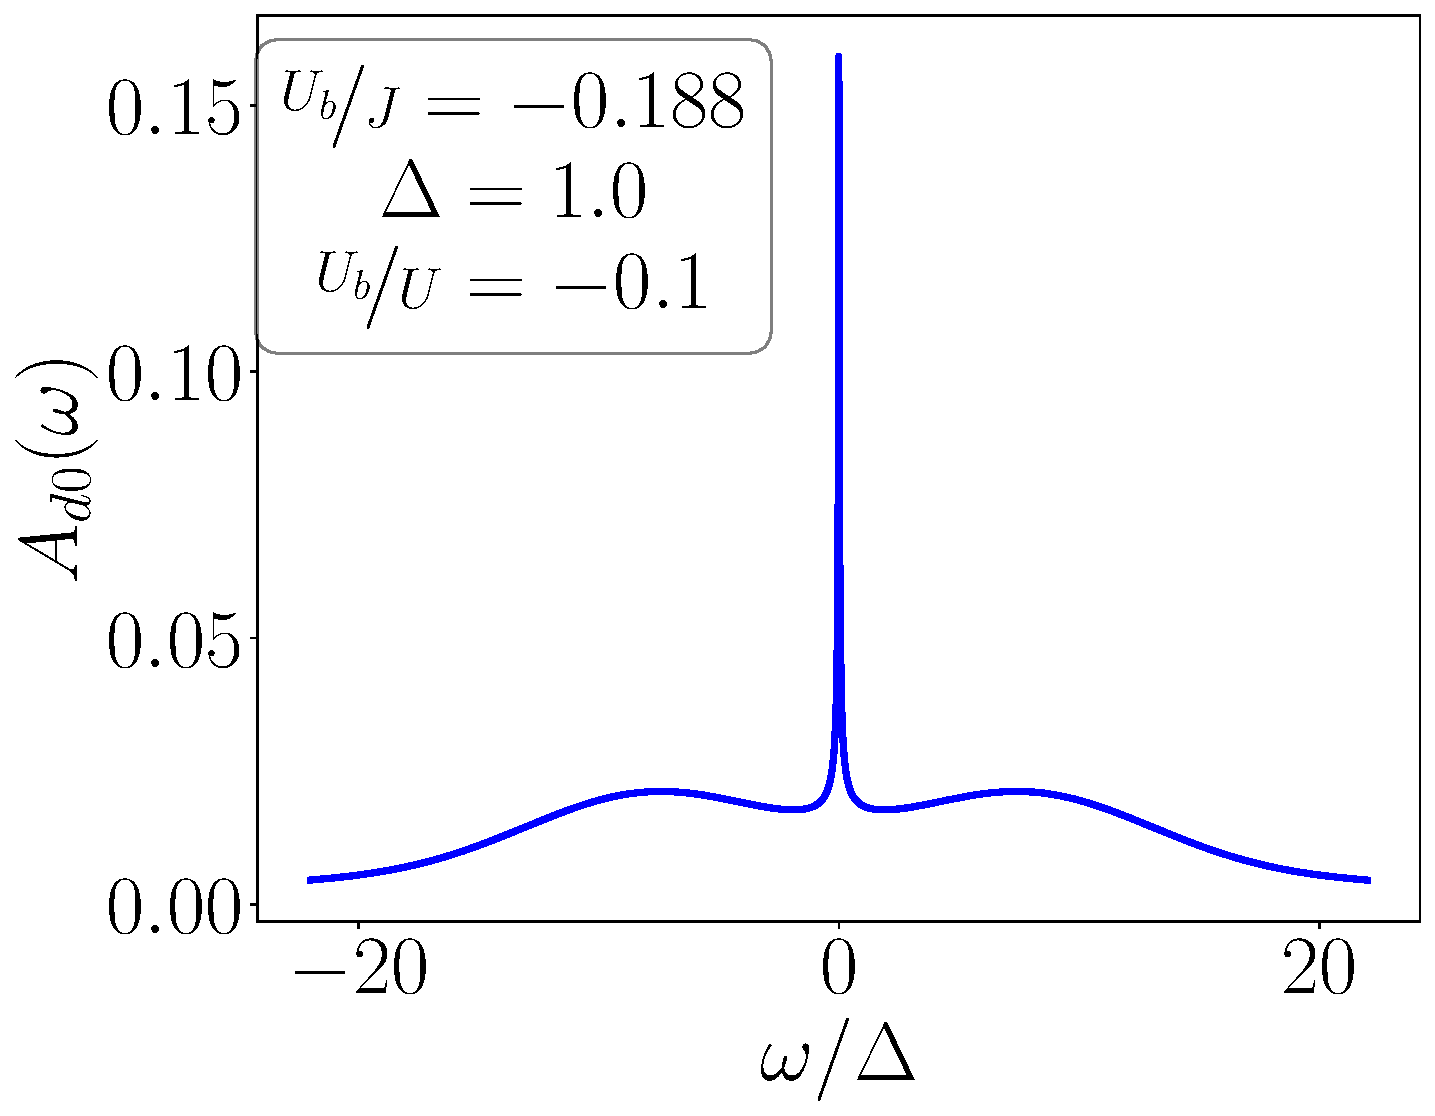
\includegraphics[width=0.45\textwidth]{../figures/spec_func_d0_Ub_by_J=-0.188.pdf}
	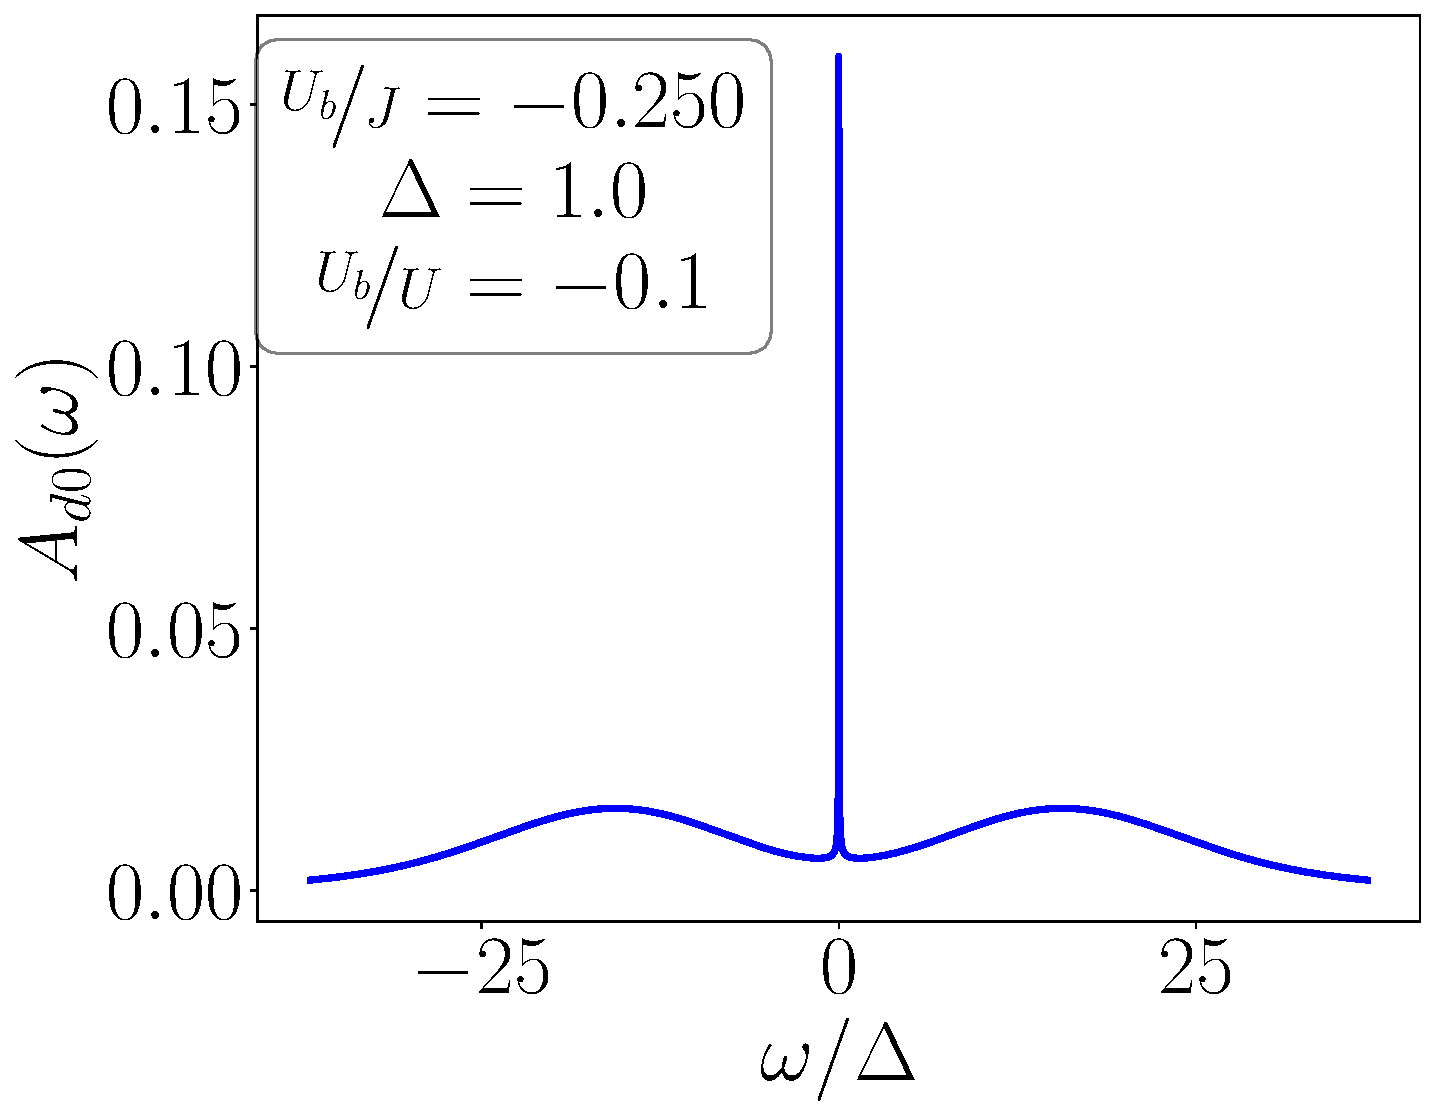
\includegraphics[width=0.45\textwidth]{../figures/spec_func_d0_Ub_by_J=-0.250.pdf}
	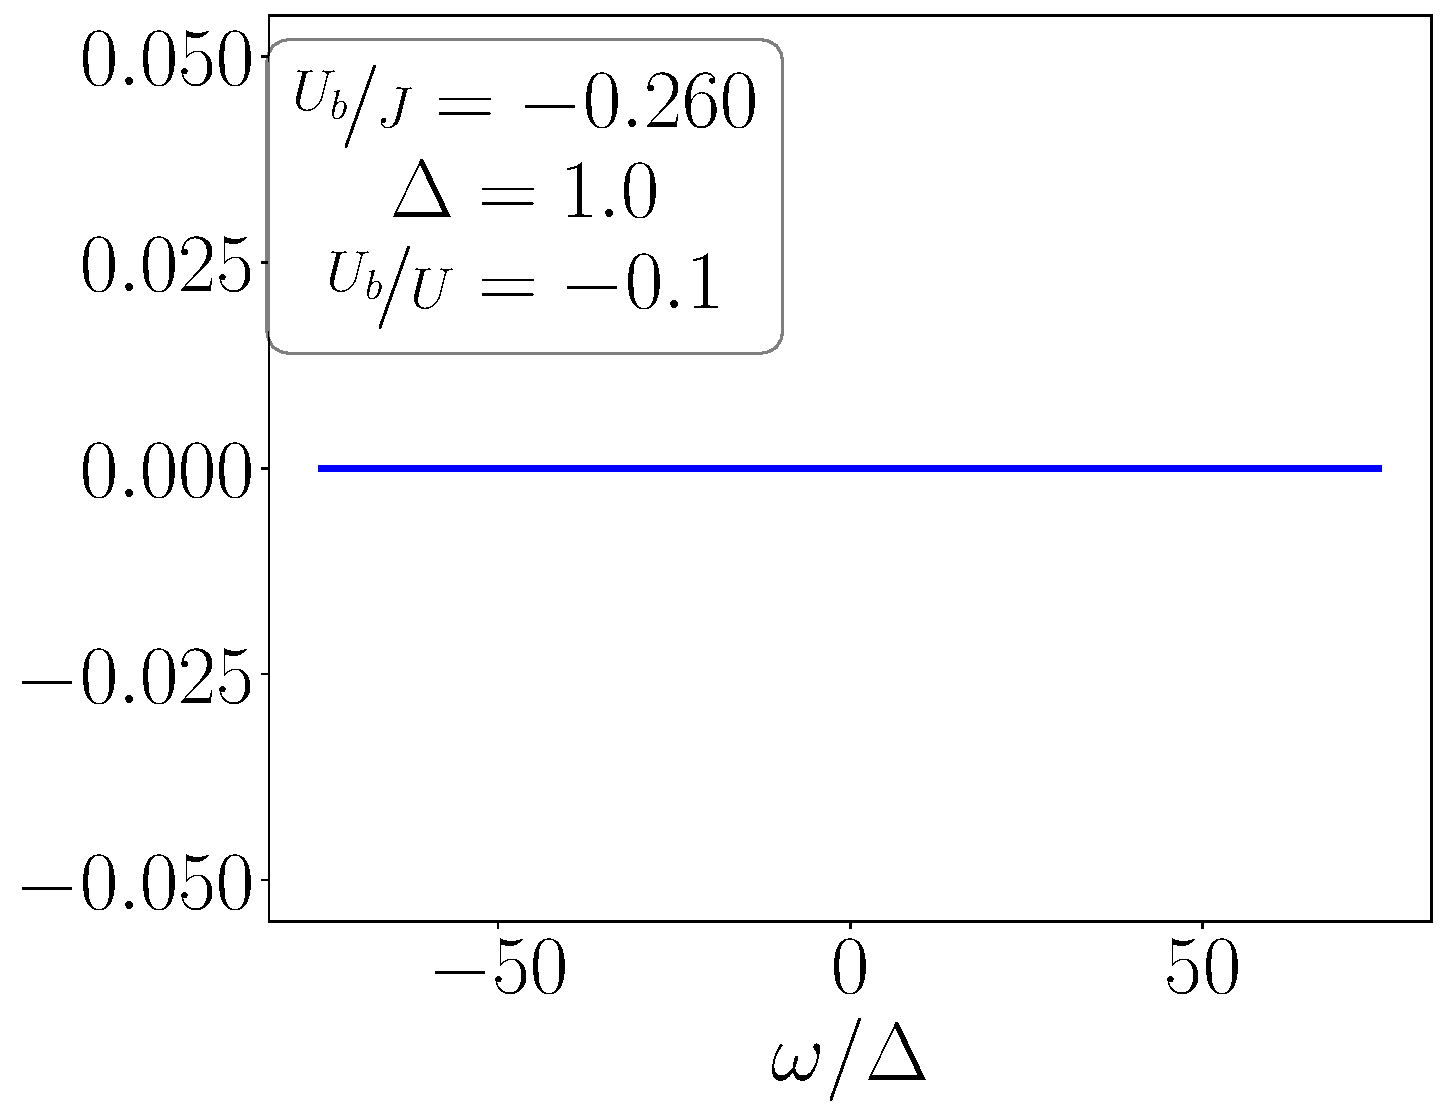
\includegraphics[width=0.45\textwidth]{../figures/spec_func_d0_Ub_by_J=-0.26.pdf}
\end{center}

\subsection{Width of central peak of \(A_{dd}\)}

\begin{center}
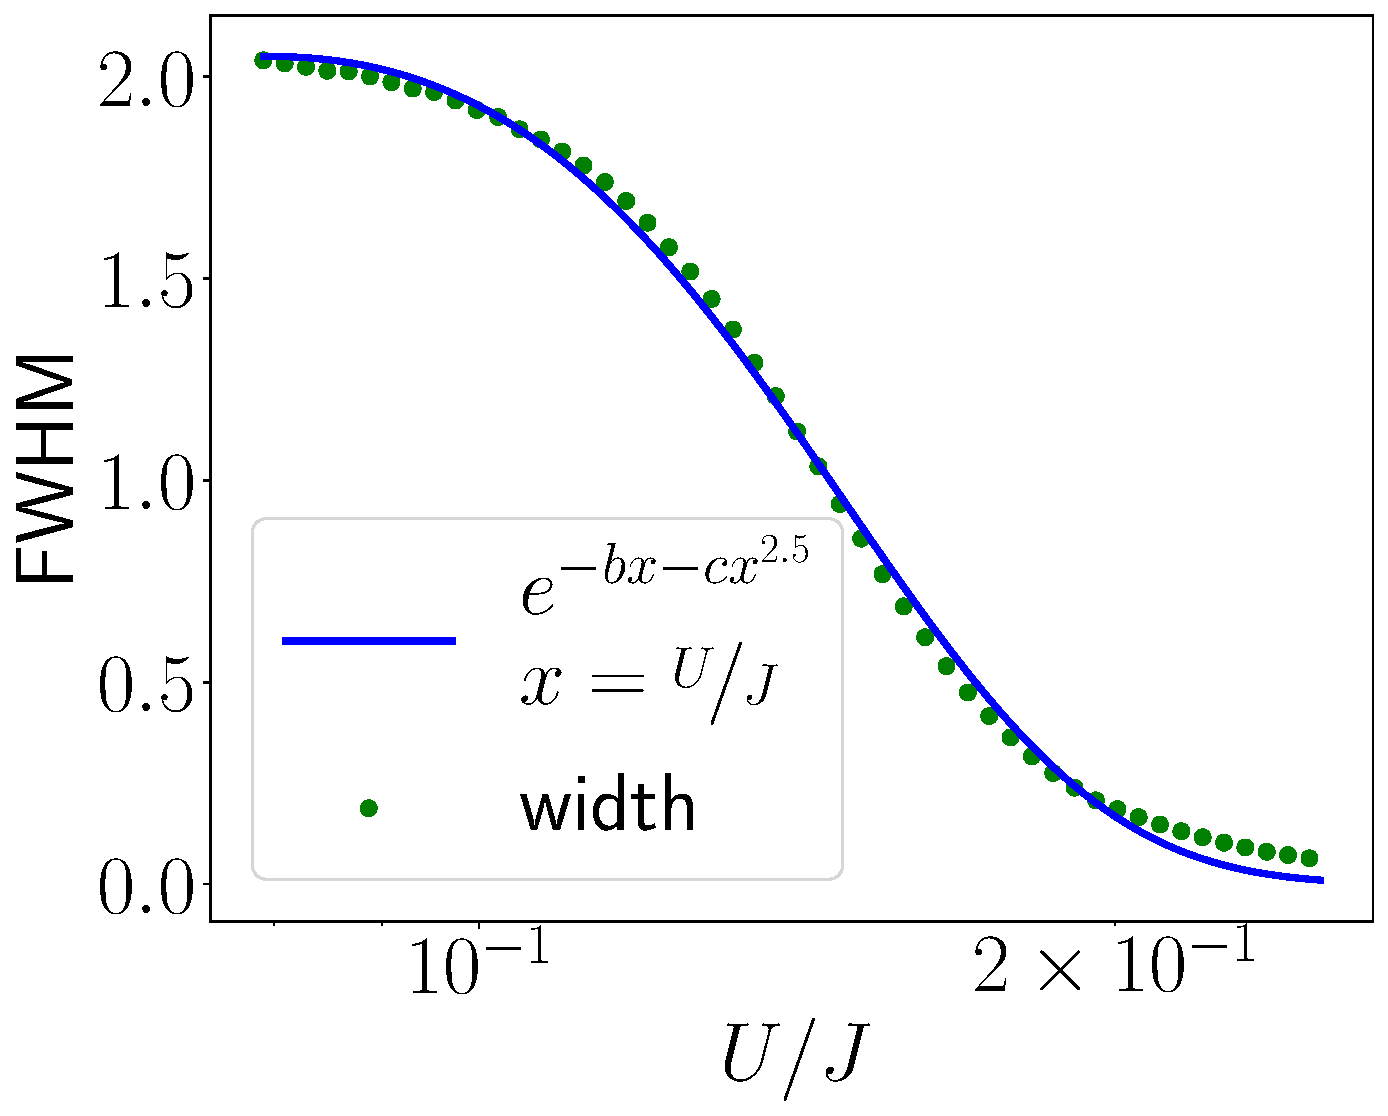
\includegraphics[width=0.45\textwidth]{../figures/spec_func_width_fit.pdf}
\end{center}

\section{Bath spectral function \(A_{00}(\omega)\) and the relation to DMFT}
In order to calculate the spectral function \(A_{00}(\omega)\) of the site connected to the impurity (referred to as the zeroth site), we will use the following strategy. We will decouple the impurity states from the fixed point Hamiltonian using a single URG transformation. This will of course generate correlations on the zeroth site. The resulting Hamiltonian will be an Anderson impurity model with the hopping between the zeroth site and the rest of the chain acting as the effective hybridisation. Schematically, we will have
\begin{equation}\begin{aligned}
	H^* = H_\text{imp} + V_\text{imp-0} + H_\text{0} + H_\text{0-1} + H_\text{rest} ~ \mathlarger{\xrightarrow{\text{decouple imp.}}} ~ E_\text{imp} + \tilde H_\text{0} + H_\text{0-1} + H_\text{rest} = H_\text{new imp} \\
	+ V_\text{new imp - rest} + H_\text{rest}
\end{aligned}\end{equation}

Since the impurity is not coupled with any site beyond the zeroth site, the parts of the Hamiltonian that involve "rest" will not change in the process. This also means that the decoupling can be performed by looking at the smaller Hamiltonian
\begin{equation}\begin{aligned}
	H_\text{imp+0} = H_\text{imp} + H_\text{0} + V_\text{imp-0} = -\frac{U^*}{2}\left( \hat n_{d \uparrow} - \hat n_{d \downarrow} \right)^2 - U_b \left( \hat n_{0 \uparrow} - \hat n_{0 \downarrow} \right)^2 + J^*S_d^z S_0^z + {V^*}\sum_\sigma \left(c^\dagger_{d\sigma}c_{0\sigma} + \text{h.c.}\right) \\
	+ \frac{J^*}{2}\left( c^\dagger_{d \uparrow}c_{d \downarrow} c^\dagger_{0 \downarrow} c_{0 \uparrow} + \text{h.c.} \right) 
\end{aligned}\end{equation}

\subsection{Renormalisation from \({V^*}\)}
From the off-diagonal term involving \({V^*}\), we generate the following term, in the particle sector for \(0\):
\begin{equation}\begin{aligned}
	{V^*} \sum_\sigma c^\dagger_{0\sigma}c_{d\sigma} \frac{1}{\tilde \omega - H_d} {V^*} c^\dagger_{d\sigma}c_{0\sigma} = |V^*|^2 \sum_\sigma c^\dagger_{0\sigma}c_{d\sigma} \frac{1}{\tilde \omega + \frac{U^*}{2}\left( 1 - \hat n_{d\bar\sigma} \right)^2 + U_b \hat n_{0\bar\sigma} + \frac{J^*}{4}\left( 1 - \hat n_{d\bar\sigma} \right) \hat n_{0\bar\sigma} } c^\dagger_{d\sigma}c_{0\sigma}
\end{aligned}\end{equation}
where \(\tilde \omega\) is the quantum fluctuation operator for the impurity site and \(H_d = -\frac{U^*}{2}\left( \hat n_{d \uparrow} - \hat n_{d \downarrow} \right)^2 - U_b \left( \hat n_{0 \uparrow} - \hat n_{0 \downarrow} \right)^2 + J^*S_d^z S_0^z \), is the diagonal part of the Hamiltonian for the imp+0 system. In order to resolve the operators in the denominator, we expand the unity in the numerator using the identity \(1 = \hat n_{d\bar\sigma}\hat n_{0\bar\sigma} + \hat n_{d\bar\sigma}\hat h_{0\bar\sigma} + \hat h_{d\bar\sigma}\hat n_{0\bar\sigma} + \hat h_{d\bar\sigma}\hat h_{0\bar\sigma}\), where \(\hat h = 1 - \hat n\) is hole operator. On Substituting this, we get
\begin{equation}\begin{aligned}
	\sum_\sigma {V^*} c^\dagger_{0\sigma}c_{d\sigma} \frac{1}{\tilde \omega - H_d} {V^*} c^\dagger_{d\sigma}c_{0\sigma} &= |V^*|^2 \sum_\sigma c^\dagger_{0\sigma}c_{d\sigma} \frac{\hat h_{d\bar\sigma}\hat h_{0\bar\sigma} + \hat h_{d\bar\sigma}\hat n_{0\bar\sigma} + \hat n_{d\bar\sigma}\hat h_{0\bar\sigma} + \hat n_{d\bar\sigma}\hat n_{0\bar\sigma}}{\tilde \omega + \frac{U^*}{2}\hat h_{d\bar\sigma} + U_b \hat n_{0\bar\sigma} + \frac{J^*}{4}\hat h_{d\bar\sigma} \hat n_{0\bar\sigma} } c^\dagger_{d\sigma}c_{0\sigma}\\
															    &= |V^*|^2 \sum_\sigma \hat h_{d\sigma} \hat n_{0\sigma}\left[\frac{\hat h_{d\bar\sigma}\hat h_{0\bar\sigma}}{\tilde\omega_{00} + \frac{U^*}{2}} + \frac{\hat h_{d\bar\sigma}\hat n_{0\bar\sigma}}{\tilde\omega_{01} + \frac{U^*}{2} + U_b + \frac{J^*}{4}} + \frac{\hat n_{d\bar\sigma}\hat h_{0\bar\sigma}}{\tilde\omega_{10}} + \frac{\hat n_{d\bar\sigma}\hat n_{0\bar\sigma}}{\tilde\omega_{11} + U_b}\right]
\end{aligned}\end{equation}
\(\tilde\omega_{(0,1),(0,1)}\) represents the quantum fluctuation scale corresponding to the configuration in the numerator.

In order to "freeze" the impurity dynamics, we will substitute \(\hat n_{d\sigma} = \hat n_{d\bar\sigma} = \frac{1}{2}\), because of the \(\mathbb{Z}_2\) symmetry and the particle-hole symmetry of the impurity levels. This gives
\begin{equation}\begin{aligned}
	\frac{1}{4}|V^*|^2 \sum_\sigma \hat n_{0\sigma} \left[\frac{\hat h_{0\bar\sigma}}{\tilde\omega_{00} + \frac{U^*}{2}} + \frac{\hat n_{0\bar\sigma}}{\tilde\omega_{01} + \frac{U^*}{2} + U_b + \frac{J^*}{4}} + \frac{\hat h_{0\bar\sigma}}{\tilde\omega_{10}} + \frac{\hat n_{0\bar\sigma}}{\tilde\omega_{11} + U_b}\right]
\end{aligned}\end{equation}

The state that most closely represents the metallic ground state is \(\bar \omega_{10}\), we take that as the reference quantum fluctuation scale \(\bar\omega\). It is of the order of \(\bar\omega \sim -\frac{J^*}{4} - \frac{U^*}{2} - U_b\). We will now relate the other scales to \(\bar\omega\) by expressing them in terms of the energy of the initial state:
\begin{equation}\begin{aligned}
	\tilde\omega_{00} \sim -U_b = \bar\omega + \frac{J^*}{4} + \frac{U^*}{2}, ~~ \tilde\omega_{01} \sim 0 = \bar\omega + \frac{J^*}{4} + \frac{U^*}{2} + U_b, ~~ \tilde\omega_{11} \sim -\frac{U^*}{2} = \bar\omega + \frac{J^*}{4} + U_b
\end{aligned}\end{equation}
Substituting these gives
\begin{equation}\begin{aligned}
	\frac{1}{4}|V^*|^2 \sum_\sigma \hat n_{0\sigma} \left[\hat h_{0\bar\sigma}\alpha_1 + \hat n_{0\bar\sigma}\alpha_2\right]
\end{aligned}\end{equation}
where \(\alpha_1 = \left(\bar\omega + U^* + \frac{J^*}{4}\right)^{-1} + \left(\bar\omega\right)^{-1}\) and \(\alpha_2 = \left(\bar\omega + U^* + 2U_b + \frac{J^*}{2}\right)^{-1} + \left(\bar\omega + 2U_b + \frac{J^*}{4}\right)^{-1}\).

Because of the particle-hole symmetry on the impurity as well as in the bath, the renormalisation from the hole sector is obtained simply by transforming \(\hat n \leftrightarrow \hat h\):
\begin{equation}\begin{aligned}
	\frac{1}{4}|V^*|^2 \sum_\sigma \hat h_{0\sigma} \left[\hat n_{0\bar\sigma}\alpha_1 + \hat h_{0\bar\sigma}\alpha_2\right]
\end{aligned}\end{equation}

The total renormalisation arising from \(V\) is therefore
\begin{equation}\begin{aligned}
	\frac{1}{4}|V^*|^2 \sum_\sigma \left[\alpha_1 \left( \hat n_{0\sigma}\hat h_{0\bar\sigma} + \hat h_{0\sigma}\hat n_{0\bar\sigma}\right) + \alpha_2 \left( \hat n_{0\sigma}\hat n_{0\bar\sigma} + \hat h_{0\sigma}\hat h_{0\bar\sigma}\right)\right] = \frac{1}{2}|V*|^2 \left(\alpha_1 - \alpha_2\right) \left(\hat n_{0 \uparrow} - \hat n_{0 \downarrow}\right)^2 + \text{constant}
\end{aligned}\end{equation}

\subsection{Renormalisation from \(J\)}
The renormalisation arising from decoupling the Kondo coupling has two terms. The first term arises when the spin of the zeroth site is initially up:
\begin{equation}\begin{aligned}
	\frac{{J^*}^2}{4}c^\dagger_{d \downarrow}c_{d \uparrow} c^\dagger_{0 \uparrow}c_{0 \downarrow} \frac{1}{\tilde \omega - H_d} c^\dagger_{0 \downarrow}c_{0 \uparrow} c^\dagger_{d \uparrow}c_{d \downarrow} = c^\dagger_{d \downarrow}c_{d \uparrow} c^\dagger_{0 \uparrow}c_{0 \downarrow} \frac{{J^*}^2/4}{\tilde \omega + \frac{U^*}{2} + U_b + \frac{J^*}{4}} c^\dagger_{0 \downarrow}c_{0 \uparrow} c^\dagger_{d \uparrow}c_{d \downarrow} = \frac{{J^*}^2}{4}\frac{\hat n_{d \downarrow} \hat h_{d \uparrow} \hat n_{ 0 \uparrow} \hat h_{0 \downarrow}}{\tilde \omega + \frac{U^*}{2} + U_b + \frac{J^*}{4}} 
\end{aligned}\end{equation}
The quantum fluctuation scale \(\tilde \omega\) for this process can be similarly related to \(\bar\omega\): \(\tilde\omega \sim -\frac{U^*}{2} - U_b - \frac{J^*}{4} = \bar\omega\). This gives
\begin{equation}\begin{aligned}
	\frac{{J^*}^2}{4}\frac{\hat n_{d \downarrow} \hat h_{d \uparrow} \hat n_{ 0 \uparrow} \hat h_{0 \downarrow}}{\bar\omega + \frac{U^*}{2} + U_b + \frac{3J^*}{4}} = \frac{{J^*}^2}{16}\frac{\hat n_{ 0 \uparrow} \hat h_{0 \downarrow}}{\bar\omega + \frac{U^*}{2} + U_b + \frac{J^*}{4}}
\end{aligned}\end{equation}
as the renormalisation for this configuration. At the final step, we substituted \(\hat n_{d\sigma} = \hat h_{d\sigma} = \frac{1}{2}\). For the other configuration where the spin of the zeroth site is down, we get
\begin{equation}\begin{aligned}
	\frac{{J^*}^2}{16}\frac{\hat n_{ 0 \downarrow} \hat h_{0 \uparrow}}{\bar\omega + \frac{U^*}{2} + U_b + \frac{J^*}{4}}
\end{aligned}\end{equation}
Adding both sectors, we get
\begin{equation}\begin{aligned}
	\frac{{J^*}^2}{16}\frac{1}{\bar\omega + \frac{U^*}{2} + U_b + \frac{J^*}{4}} \left(\hat n_{ 0\uparrow} - \hat n_{0 \downarrow}\right)^2
\end{aligned}\end{equation}

\subsection{Total renormalisation}
Adding the contributions from both \(V^*\) and \(J^*\),  the net renormalisation is the generation of a local correlation term \(-U_0\left(\hat n_{ 0\uparrow} - \hat n_{0 \downarrow}\right)^2\) on the zeroth site, where \(U_0\) is given by
\begin{equation}\begin{aligned}
	U_0 = -\frac{{J^*}^2}{16}\frac{1}{\bar\omega + \frac{U^*}{2} + U_b + \frac{J^*}{4}} - \frac{1}{2}|V^*|^2\left(\frac{1}{\bar\omega + U^* + \frac{J^*}{4}} + \frac{1}{\bar\omega} - \frac{1}{\bar\omega + U^* + 2U_b + \frac{J^*}{2}} - \frac{1}{\bar\omega + 2U_b + \frac{J^*}{4}}\right) 
\end{aligned}\end{equation}

The effective Hamiltonian for the zeroth site is therefore
\begin{equation}\begin{aligned}
	H_\text{0+rest} = \underbrace{-\left(U_0 + U_b\right)\left(\hat n_{0\uparrow} - \hat n_{0\downarrow}\right)^2}_\text{new correlated impurity} \underbrace{- t\sum_{j\in \text{n.n. of 0},\atop{\sigma}}\left(c^\dagger_{0\sigma}c_{j\sigma} + \text{h.c.}\right)}_\text{hopping between new impurity \& new bath} \underbrace{-t \sum_{\left<i,j \right>}\left(c^\dagger_{i\sigma}c_{j\sigma} + \text{h.c.}\right)}_\text{K.E. of new bath}
\end{aligned}\end{equation}

\subsection{Equivalence of the impurity site and the zeroth site: towards self-consistency}
The fact that we end up with an Anderson impurity model shows that the behaviour of the zeroth site is equivalent to that of a correlated impurity interacting with a conduction bath through single-particle hopping. The correlation for this impurity is given by \(U_\text{eff} = U_0 + U_b\), while the effective hybridisation for this new impurity into the conduction bath is given by \(V = -t\). The new conduction bath is formed by all the sites of the lattice apart from the zeroth site. From Fig.~\ref{pair_fluc}, we know that the the spin-flip correlations are quite dominant up to the transition, indicating that the largest energy scale in the system at low-energies is \(J^*\). Using this, the effective correlation can be expressed to leading order as
\begin{equation}\begin{aligned}
	U_\text{eff} \simeq \frac{J^*}{8}
\end{aligned}\end{equation}
This is simply a restatement of the fact that upto the transition, the impurity spectral function displays a central peak~(Fig.~\ref{spec_func_fig}); it is the dominant spin-flip scattering processes that lead to both the central peak as well as the induced repulsive correlation \(U_\text{eff}\) at the zeroth site. This also indicates that the bath spectral function will have a similar central peak, owing to the same scattering processes. We conclude that the spin-exchange coupling \(J\) acts as a mechanism of symmetrisation between the impurity and zeroth sites, leading to similar effective local correlations and similar local spectral functions. This also suggests that the self-consistency-based approach towards a bulk model, as used in DMFT, effectively involves finding the impurity model that has identical behaviour across the impurity and zeroth sites. Indeed, such an idea has been used in Ref.~\cite{moeller_1995} to study the behaviour of the Hubbard model near the transition. 

In the spirit of Ref.~\cite{moeller_1995}, near the transition, we can integrate out the charge degrees of freedom of the Anderson model via a canonical Schrieffer-Wolff transformation. Upto second order, this transformation removes the on site correlation \(U\) and the single-particle hybridisation \(V\) by generating an additional spin-exchange term \(J^\prime \sim \frac{V^2}{U+U_b}\). The total s-d coupling then becomes \(\widetilde J = J + J^\prime\), and the effective Hamiltonian after the transformation is
\begin{equation}\begin{aligned}
	H_\text{Kondo} = \widetilde J \vec{S}_d\cdot\vec{S}_0 - U_b\left( \hat n_{0 \uparrow} - \hat n_{0 \downarrow} \right)^2 + H_\text{K.E.}
\end{aligned}\end{equation}
In this simplified model, the RG equations for \(\widetilde J\) and \(U_b\) can be obtained simply by setting \(U =V = 0\) in the more general RG equations ~\ref{rg-eq1} through \ref{rg-eq3}:
\begin{equation}\begin{aligned}
	\Delta \widetilde J = -\frac{n_j \widetilde J\left(\widetilde J + 4U_b\right)}{d_2},~~ \Delta U_b = 0
\end{aligned}\end{equation}
This makes it clear that the metal-insulator transition in this model is driven by the competition between Kondo screening generated by \(\tilde J\) and local pair correlation in the bath produced by \(U_b = -|U_b|\). The fact that the only major impurity-bath interaction near the transition is of the spin-exchange kind reiterates the fact that the correlated spin-flip processes play the most important role in the model, and leads to the symmetrisation between the impurity and zeroth sites.

\section{What, then, are the minimal ingredients for a metal-insulator transition?}
We now return to the question posed at the very beginning in section~\ref{sec:min_model}: What is the minimal auxiliary model that can demonstrate a metal-insulator transition in the bulk? To answer this question, we first recall all the relevant RG equations in the positive \(U\) regime:
\begin{gather}
	\Delta U_b = 0, ~ ~\Delta U = 4V^2 n_j\left(\frac{1}{d_1} - \frac{1}{d_0}\right) - n_j\frac{J^2}{d_2},\\
	\Delta V = -\frac{3n_j V}{8}\left[\left(J + 4U_b/3\right) \left(\frac{1}{d_2} + \frac{1}{d_1}\right) + 4U_b/3\left(\frac{1}{d_3} + \frac{1}{d_0}\right)\right],\\
	\Delta J = -\frac{n_j J\left(J + 4U_b\right)}{d_2}~.
\end{gather}
where \(d_1 > d_2 > d_3 > d_0\).
We now consider various models with increasing number of parameters.

\subsection{Only impurity correlation and hybridisation \(U,V\)}
If we had only \(U\) and \(V\), the RG equations simplify to
\begin{equation}\begin{aligned}
	\Delta U = 4V^2 n_j\left(\frac{1}{d_1} - \frac{1}{d_0}\right) < 0,~ ~ ~\Delta V = 0
\end{aligned}\end{equation}
\(U\) is irrelevant while the hybridisation \(V\) is marginal, so the fixed point is where the impurity is screened. The bulk model will always be metallic. There is no transition in such a model.

\subsection{Impurity correlation, hybridisation and spin-exchange between impurity and bath \(U,V,J\)}
If we now add a spin-exchange coupling \(J\) between the impurity and the bath into the Hamiltonian, we obtain the extended SIAM studied in chapter~\ref{esiam-urg}. As discussed in that chapter, this is again similar to the previous case - the only stable fixed point is one of strong-coupling, and the bulk metal will never have an insulating phase.

\subsection{Impurity correlation, hybridisation and local pairing interaction on the bath \(U,V,U_b\)}
If we replace the \(J\) with an local interaction \(U_b\) on the bath, the RG equations undergo some changes:
\begin{gather}
	\Delta U_b = 0, ~ ~\Delta U = 4V^2 n_j\left(\frac{1}{d_1} - \frac{1}{d_0}\right) = \frac{4V^2U}{\left(\omega - D/2 + U_b/2\right)^2 - U^2/4},\\
	\Delta V = -n_j V U_b\left[\frac{\omega - D/2 + U_b/2}{\left(\omega - D/2 + U_b/2\right)^2 - U^2/4} + \frac{1}{\omega - D/2 + U_b/2}\right]~.
\end{gather}
This regime is interesting because it shows a variety of behaviour:
\begin{itemize}
	\item For \(U_b>0\), the correlation \(U\) is irrelevant and \(V\) is relevant. This will produce a metal (see fig.~\ref{noJ_Ub_gt_0}).
	\item For \(U_b<0\), both \(U\) and \(V\) are irrelevant, but \(V\) decays much faster than \(U\), and \(U\) saturates to a non-zero appreciable value which although lower than the bare value is much greater than 0 (see fig.~\ref{noJ_Ub_lt_0}). This behaviour is enhanced by making \(U_b\) more negative; \(V\) decays even faster to zero, while \(U\) saturates at higher values. If the bare bandwidth is increased, the fixed point value of \(U\) actually decreases, so it appears that on taking the thermodynamic limit, \(U\) renormalises to zero (see fig.~\ref{noJ_Ub_lt_0_D}).
\end{itemize}

Neither of these cases give rise to an insulator, because \(U\) never renormalises to a non-zero fixed point value in the thermodynamic limit.

\begin{center}
	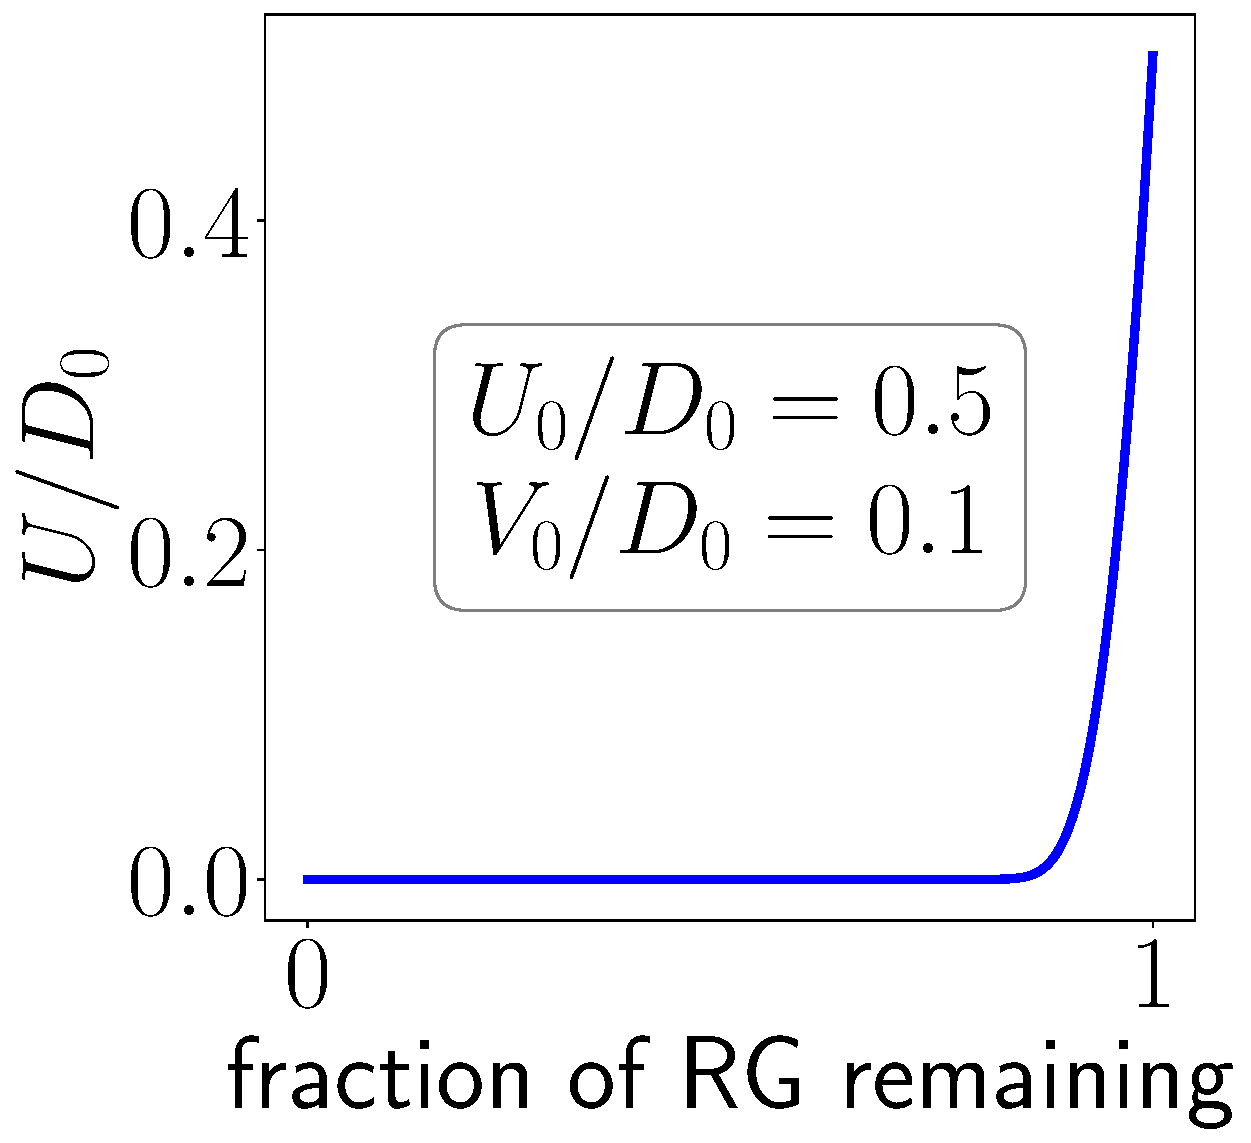
\includegraphics[width=0.4\textwidth]{../figures/no_J_Ub=0.05_D=10_U.pdf}
	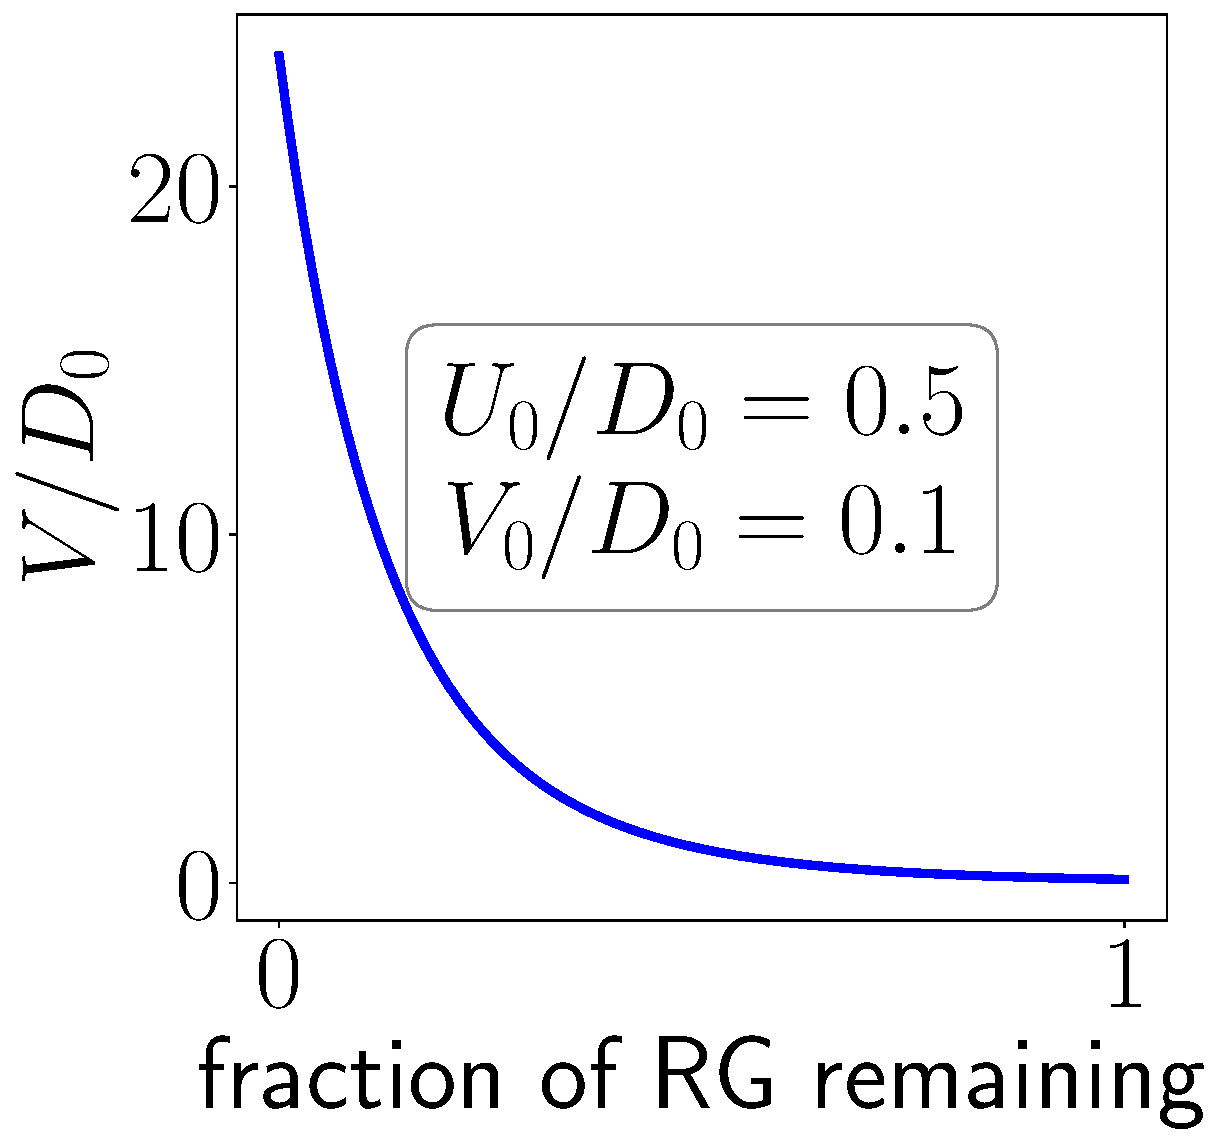
\includegraphics[width=0.4\textwidth]{../figures/no_J_Ub=0.05_D=10_V.pdf}
	\captionof{figure}{RG flows of \(U\) (left panel) and \(V\) (right panel) in the regime \(U_b>0\), for the auxiliary model with \(U,V,U_b\). The impurity correlation \(U\) is irrelevant while the hybridisation \(V\) is relevant, leading to a metallic phase in the bulk.}
	\label{noJ_Ub_gt_0}

	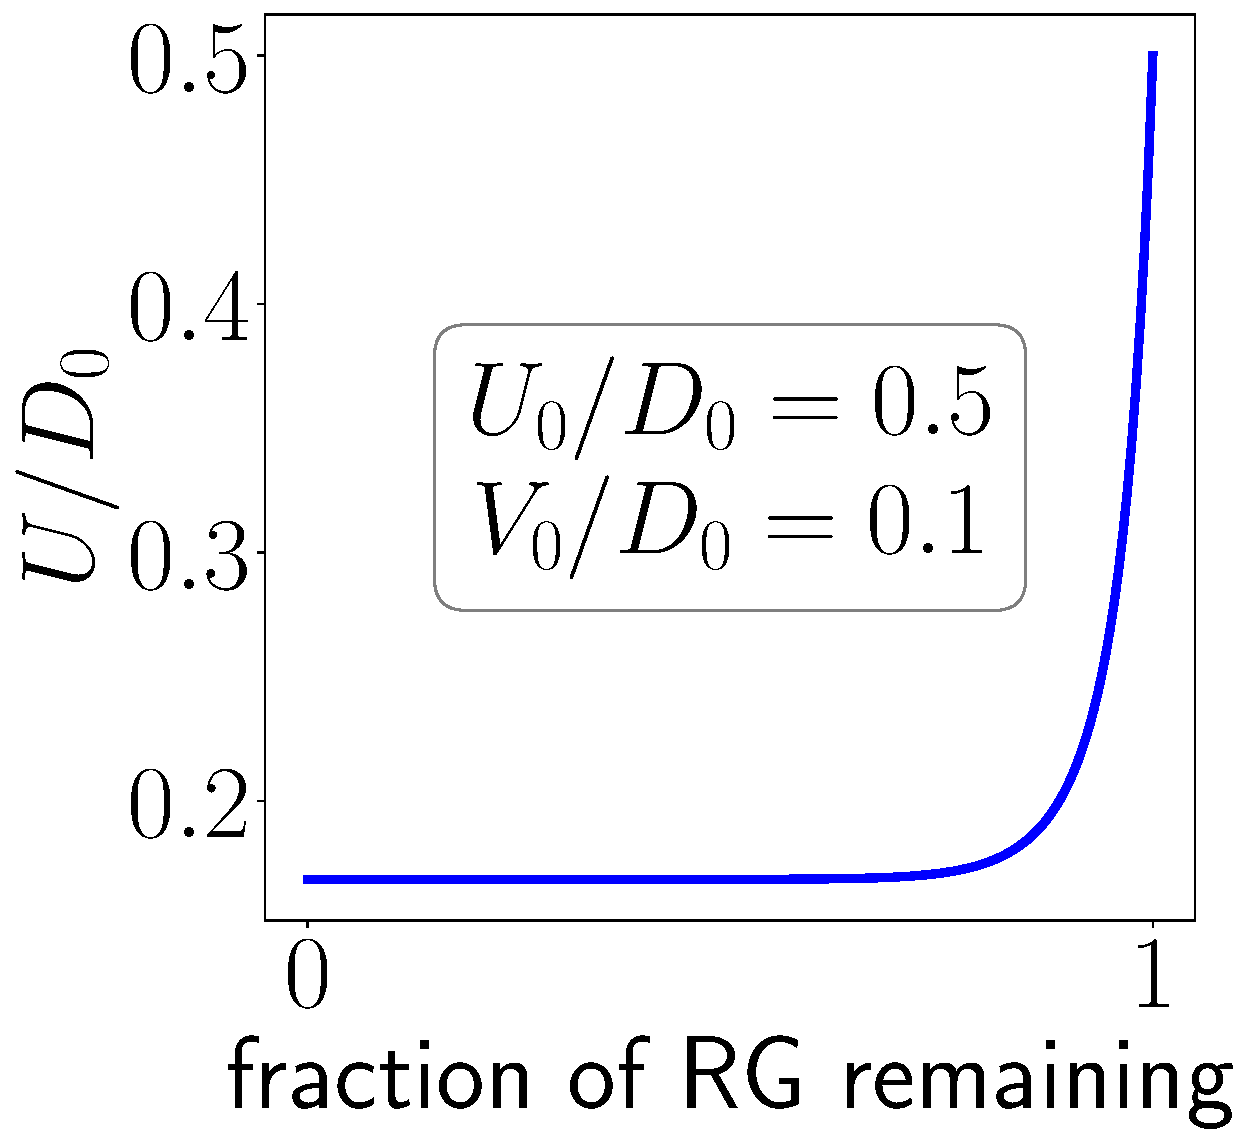
\includegraphics[width=0.4\textwidth]{../figures/no_J_Ub=-0.10_D=10_U.pdf}
	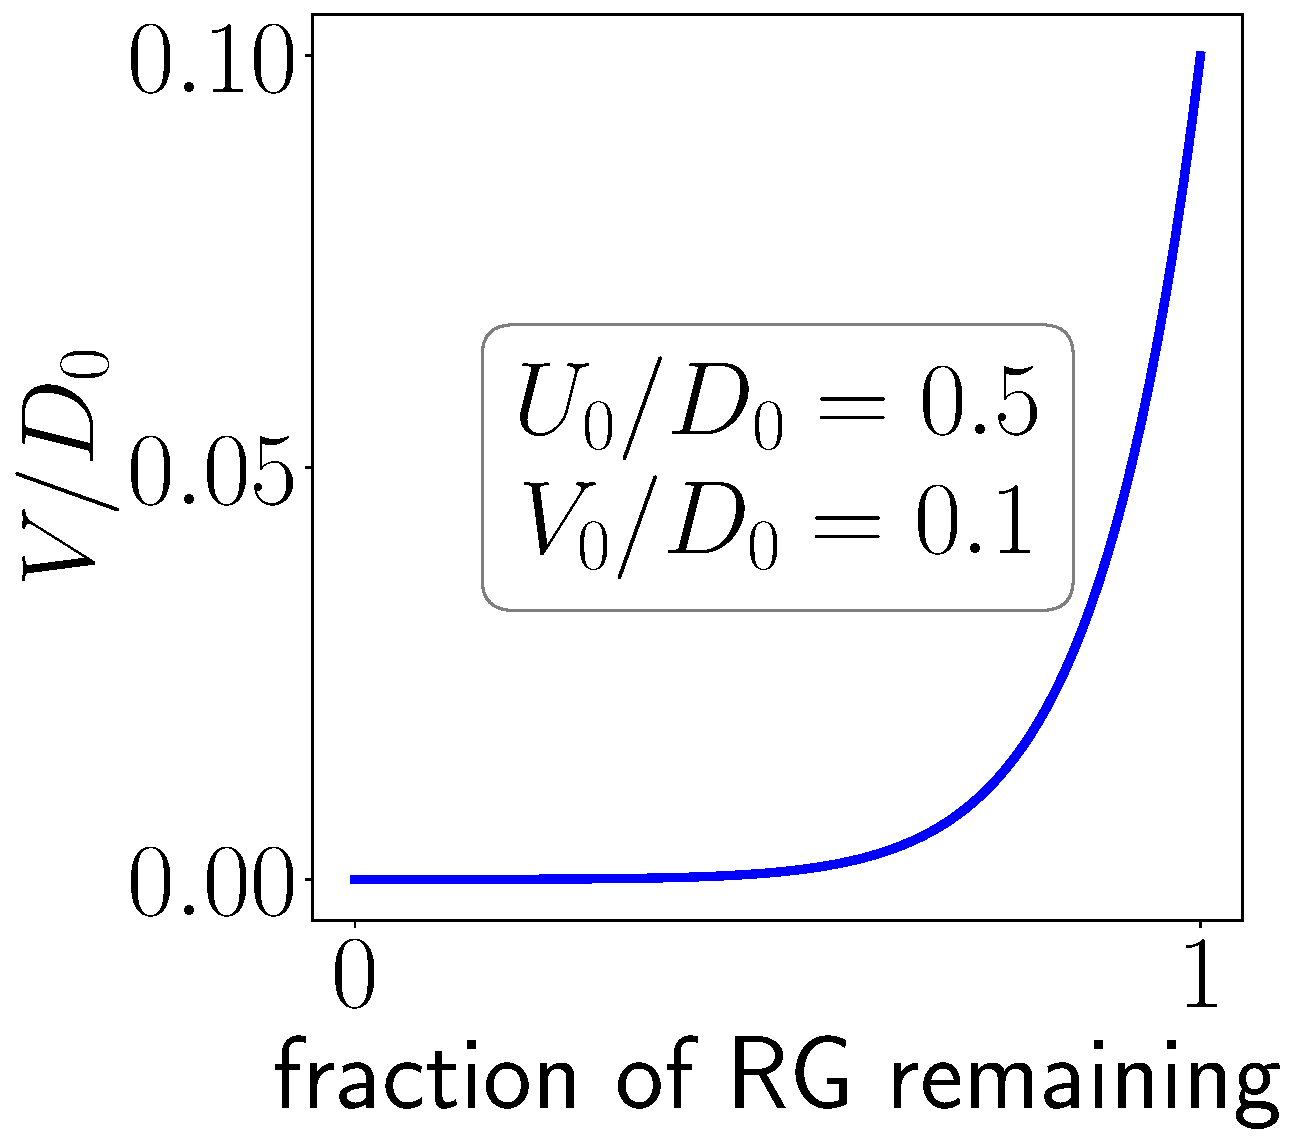
\includegraphics[width=0.4\textwidth]{../figures/no_J_Ub=-0.10_D=10_V.pdf}
	\captionof{figure}{RG flows of \(U\) (left panel) and \(V\) (right panel) in the regime \(U_b<0\), for the auxiliary model with \(U,V,U_b\). The hybridisation \(V\) is sharply irrelevant, renormalising to zero, while the impurity correlation \(U\) survives at the fixed point.}
	\label{noJ_Ub_lt_0}

	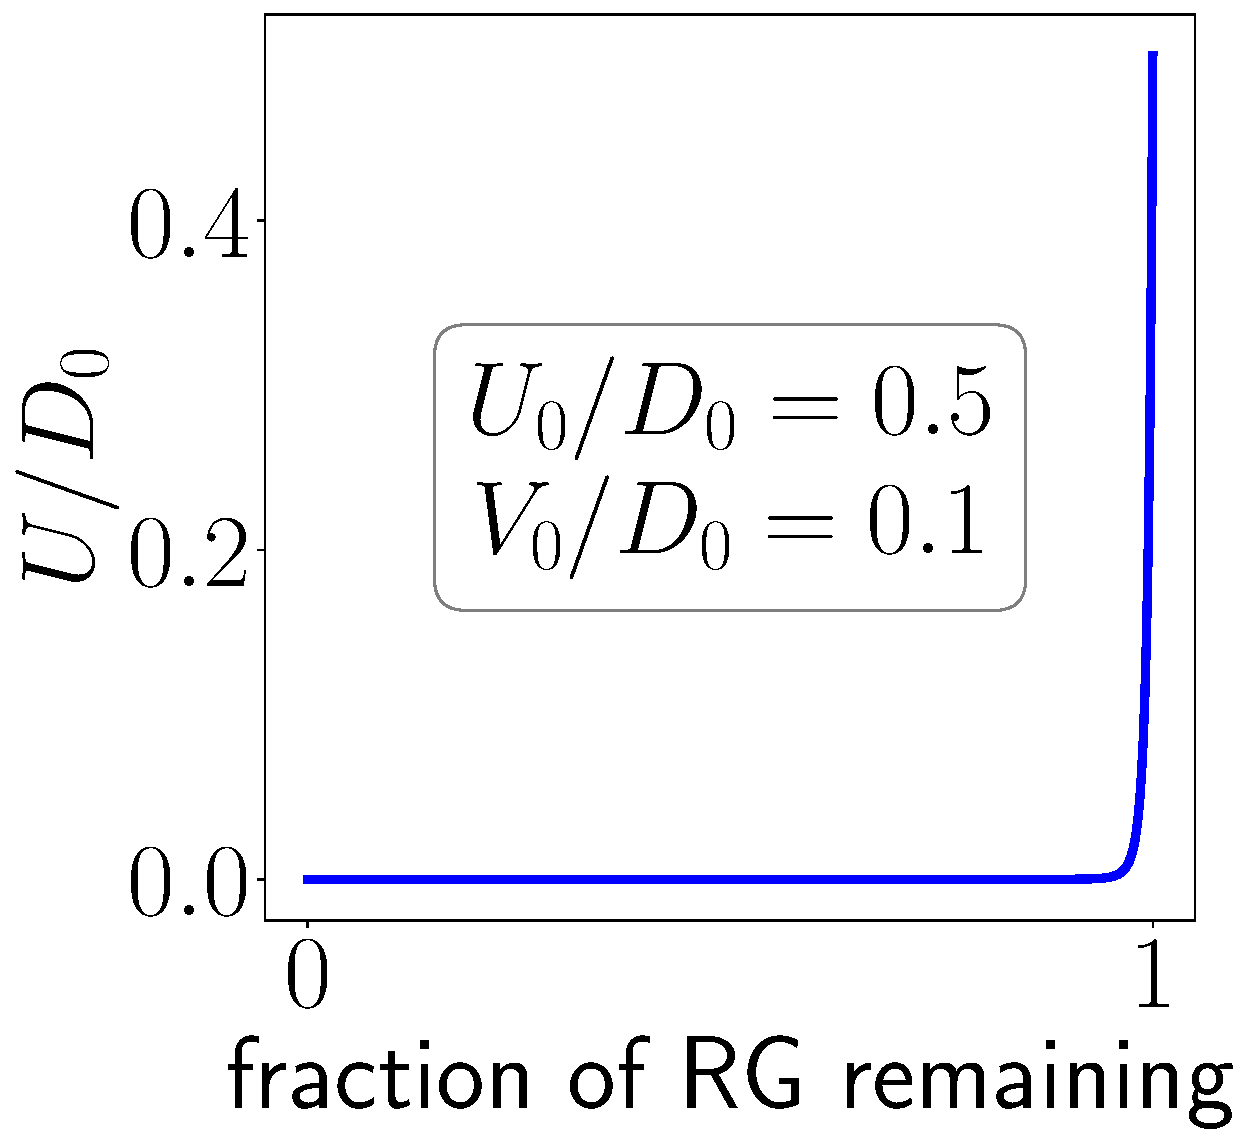
\includegraphics[width=0.4\textwidth]{../figures/no_J_Ub=-0.10_D=100_U.pdf}
	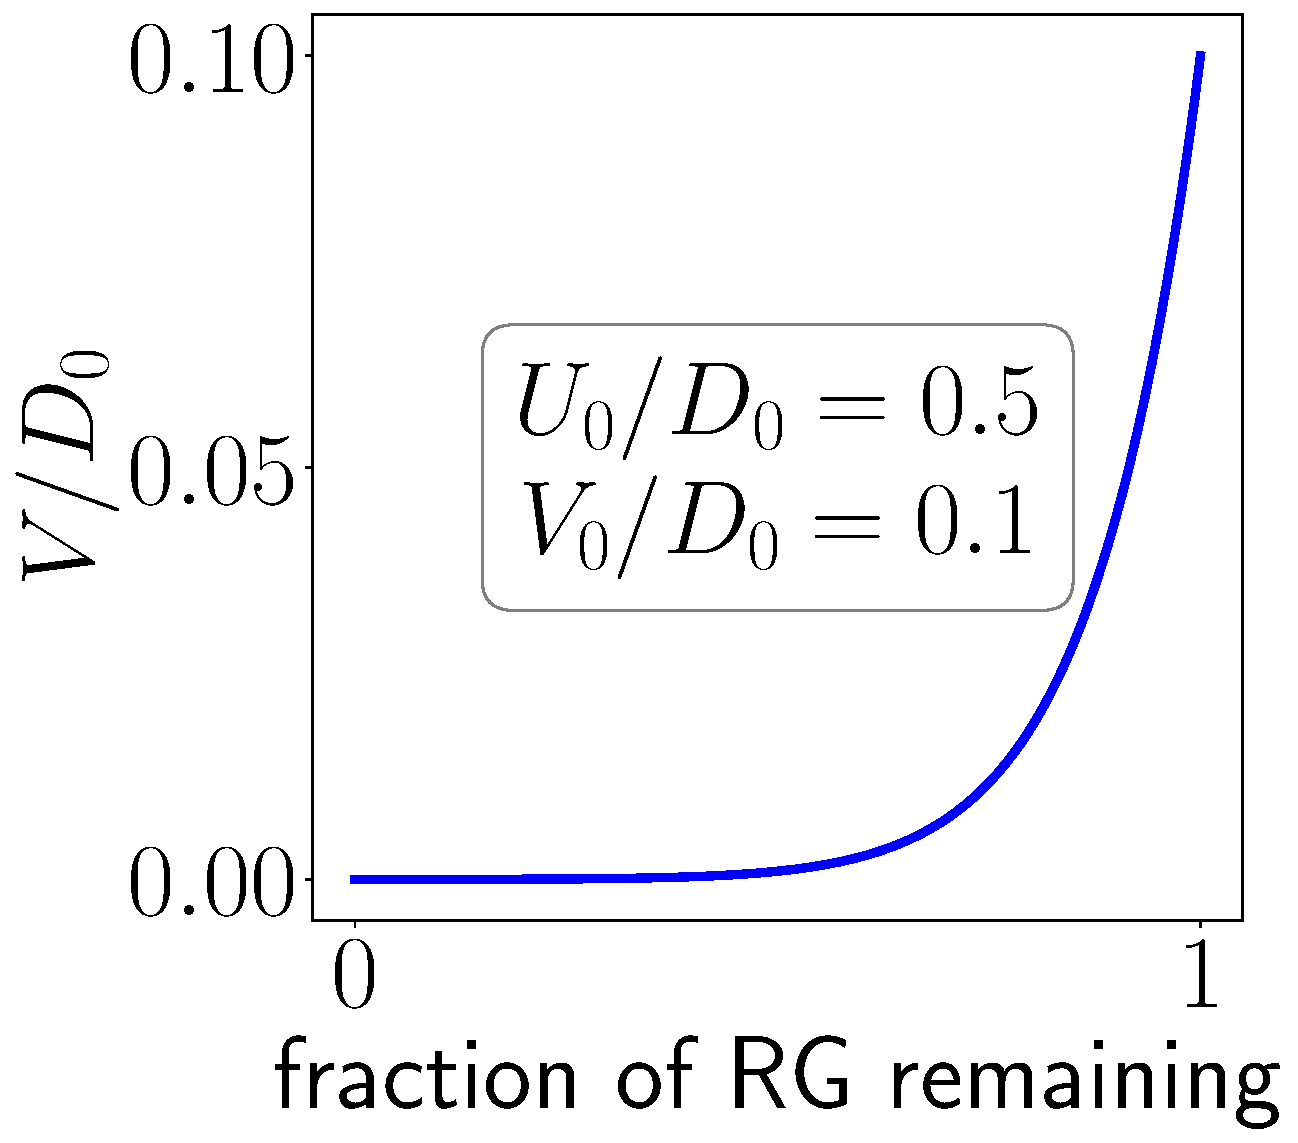
\includegraphics[width=0.4\textwidth]{../figures/no_J_Ub=-0.10_D=100_V.pdf}
	\captionof{figure}{RG flows of \(U\) and \(V\) in the regime \(U_b<0\) at a larger bandwidth, for the auxiliary model with \(U,V,U_b\).  \(U\) now renormalises to zero, so an insulator is not possible in the thermodynamic limit.}
	\label{noJ_Ub_lt_0_D}
\end{center}

\subsection{Attractive correlation \(U_b\) instead of \(V\): \(U,J,U_b\)}
In the presence of these three couplings, the RG equations become
\begin{equation}\begin{aligned}
	\Delta U = -n_j J^2/d_2,~ ~ ~ \Delta J = -n_j J(J+4U_b)/d_2
\end{aligned}\end{equation}
Since \(J > 0\), \(\Delta U\) is always positive, so \(U\) is always relevant. For \(4U_b > -J\), \(\Delta J\) is also positive, and \(J\) is relevant. We end up in a metallic phase. However, for \(4U_b < -J\), \(J\) becomes irrelevant, and the fixed point is that of a local moment decoupled from the bath, which describes an insulating state in the bulk.

\subsection{The full model?}
We are therefore ultimately led to a model with all four parameters. This was studied in chapter~\ref{siam-attr-chap}, and was shown to display both metallic and insulating phases. This makes it clear that {\it the minimal model must have all three kinds of correlation: magnetic \((U,J)\), delocalisation \((V)\) and pair formation \((U_b)\)}.
